%% LyX 2.0.0 created this file.  For more info, see http://www.lyx.org/.
%% Do not edit unless you really know what you are doing.
\documentclass[12pt, english]{kuthesis}
\usepackage{amsmath, amssymb, amsfonts}
\usepackage{mathptmx}
\renewcommand{\sfdefault}{lmss}
\renewcommand{\ttdefault}{lmtt}
\usepackage[T1]{fontenc}
\usepackage[utf8]{inputenc}
\usepackage{listings, geometry}
\geometry{verbose,tmargin=1in,bmargin=1in,lmargin=1in,rmargin=1in}
\setcounter{secnumdepth}{3}
\setcounter{tocdepth}{3}
\usepackage{color}
\usepackage{graphicx}
\usepackage[doublespacing]{setspace}
\usepackage{esint}
\usepackage[authoryear]{natbib}
\usepackage{amsthm, verbatim, bm}
\usepackage{floatrow}
\usepackage{listings}
\usepackage{mathtools}
\usepackage{calc}
\usepackage{enumitem}
\usepackage{slashbox}

\newcommand{\ds}{\displaystyle}

\newfloatcommand{capbtabbox}{table}[][\FBwidth]


\newcommand{\dfn}[1]{\textit{#1}}
\newcommand{\dc}{,\dotsc,}
\DeclareMathOperator{\vrt}{vert}
\makeatletter

%%%%%%%%%%%%%%%%%%%%%%%%%%%%%% Allow overlay of characters
\fboxsep=1pt
\newcommand{\olay}[2]{\makebox[\widthof{$#2$}][c]{$#1$}}
\newcommand{\ze}{\olay{0}{+}}


%%%%%%%%%%%%%%%%%%%%%%%%%%%%%% LyX specific LaTeX commands.
\providecommand{\LyX}{L\kern-.1667em\lower.25em\hbox{Y}\kern-.125emX\@}
%% Because html converters don't know tabularnewline
\providecommand{\tabularnewline}{\\}
%% A simple dot to overcome graphicx limitations
\newcommand{\lyxdot}{.}


%%%%%%%%%%%%%%%%%%%%%%%%%%%%%% User specified LaTeX commands.

\newcommand{\tri}{\rotatebox[origin=c]{180}{\(\nabla\)}}
\newcommand{\mb}[1]{\mathbb{#1}}
\newcommand{\mc}[1]{\mathcal{#1}}
\newcommand{\mbf}[1]{\mathbf{#1}}
\newcommand{\scr}[1]{\mathcal{#1}}
\newcommand{\mf}[1]{\mathfrak{#1}}
\newcommand{\fl}[1]{\scr F(#1)}
\newcommand{\ph}{\ensuremath{\phantom{.}}}
\DeclareMathAlphabet{\mathpzc}{OT1}{pzc}{m}{it}

\newcommand{\sbset}{\subseteq}

\newcommand{\mt}{\varnothing}
\newcommand{\la}{\lambda}
\newcommand{\RR}{\mb R}
\newcommand{\Tr}[1]{{#1}^{\mathrm{T}}}
\newcommand{\R}[1]{\RR^{#1}}
\newcommand{\Sp}[1]{\mb S^{#1}}
\newcommand{\ol}[1]{\overline{#1}}
\newcommand{\wt}[1]{\widetilde{#1}}
\newcommand{\ve}[1]{\bm{#1}}
\newcommand{\brac}[1]{\left[#1\right]}
\newcommand{\floor}[1]{\left\lfloor#1\right\rfloor}
\newcommand{\ceil}[1]{\left\lceil#1\right\rceil}
\newcommand{\ip}[2]{\left\langle#1,#2\right\rangle}
\newcommand{\abs}[1]{\left\lvert#1\right\rvert}
\newcommand{\norm}[1]{\left\lVert#1\right\rVert}
\newcommand{\card}[1]{\abs{#1}}
\newcommand{\tast}{\ensuremath{\ast}}
\newcommand{\join}{\vee}
\newcommand{\N}{\mb N}
\newcommand{\B}[2]{B_{#1}\left(#2\right)}
\newcommand{\eps}{\varepsilon}
\newcommand{\usv}[5]{\Tr{\begin{bmatrix}#1 & #2 & #3 & #4 & #5\end{bmatrix}}}
\newcommand{\sv}[5]{\pm \usv#1#2#3#4#5}
\newcommand{\lb}{\right.\\ &\phantom{= \left\{.\vphantom.\right.}\left.}
\newcommand{\zmat}[2]{[0]_{\substack{#1\\ #2}} }
\newcommand{\snl}{\right. \\ &\phantom{=\Biggl\{}\left.}
\newcommand{\nv}{^{-1}}

\newcommand{\cyc}[2]{C_{#2}(#1)}                            % cyclic polytope with #1 vertices in #2 dimensions
\newcommand{\simp}[1]{\Delta_{#1}}                          % #1-simplex
\newcommand{\cube}[1]{Q_{#1}}                               % #1-cube
\newcommand{\xp}[1]{X_{#1}}                                 % #1-crosspolytope
\newcommand{\rest}[2]{\left.#1\right\vert_{#2}}             % Restriction of G to W
\newcommand{\gr}[1]{\mc G(#1)}                              % The graph of a polytope #1
\newcommand{\conn}[1]{\kappa\left(#1\right)}                % connectivity of graph #1
\newcommand{\had}[1]{h\left(#1\right)}                      % Hadwiger numberof graph #1


\newcommand{\seta}[1]{\left\{#1\right\}}
\newcommand{\setb}[2]{\seta{#1\vphantom{#1 #2}\phantom{.}\right\vert\left.\vphantom{#1 #2}#2}}

\DeclareMathOperator{\spn}{span}
\DeclareMathOperator{\conv}{conv}
\DeclareMathOperator{\rref}{rref}
\DeclareMathOperator{\relint}{relint}
\DeclareMathOperator{\dep}{dep}
\DeclareMathOperator{\aff}{aff}
\DeclareMathOperator{\Ne}{N}
\DeclareMathOperator{\Po}{P}
\DeclareMathOperator{\sign}{sign}
\DeclareMathOperator{\supp}{supp}
\DeclareMathOperator{\pyr}{pyr}
\DeclareMathOperator{\prism}{prism}
\DeclareMathOperator{\galed}{gale}
\DeclareMathOperator{\sgn}{{\textsc{sign}}}
\DeclareMathOperator{\sepn}{sep}
\DeclareMathOperator{\binlog}{lb}

\newcommand{\Neg}[1]{\Ne(#1)}
\newcommand{\Pos}[1]{\Po(#1)}
\newcommand{\sep}[2]{\sepn\left(#1,#2\right)}

%%%%%%%%%%%  Horizontal shifter
\makeatletter
\newcommand*{\shifttext}[2]{%
  \settowidth{\@tempdima}{#2}%
  \makebox[\@tempdima]{\hspace*{#1}#2}%
}
\makeatother

%%%%%%%%%% amsthm Theorem styles

% Define `Theorem', and reset its counter after each chapter increment.
\newtheorem{Theorem}{Theorem}
\makeatletter
\@addtoreset{Theorem}{thechapter}
\makeatother

% Define `Conjecture', it has no counter.
\newtheorem*{Conjecture}{Conjecture}


% Define `Corollary', and reset its counter after each theorem increment.
\newtheorem{Corollary}{Corollary}
\makeatletter
\@addtoreset{Corollary}{Theorem}
\makeatother
% Define UBT, no counter
    \newtheorem*{UBT}{Upper Bound Theorem}
% Define GEC, no counter
    \newtheorem*{GEC}{Gale's Evenness Condition}
% Define Cor, no counter
    \newtheorem*{Cor}{Corollary}

% Define `Lemma', count on the same counter as Theorem.
    \newtheorem{Lemma}[Theorem]{Lemma}

\theoremstyle{definition}
% Define `Definition' and `Definftions', no counter.
    \newtheorem*{Definition}{Definition}
    \newtheorem*{Definitions}{Definitions}
% Define `Note', no counter.
    \newtheorem*{Note}{Note}
% Define `Remark', no counter.
    \newtheorem*{Remark}{Remark}
    \newtheorem*{Question}{Question}
% Define `OpenProblem', no counter.
    \newtheorem*{OpenProblem}{Open Problem}
% Define `Example', count on the same counter as Proposition.
    \newtheorem{Example}[Theorem]{Example}
% Define `Examples', count on the same counter as Proposition.
    \newtheorem{Examples}[Theorem]{Examples}

%   Proof Sketch environment
    \newenvironment{SketchProof}{\trivlist\item[]{\sc{Sketch of Proof}}.}%
    {\unskip\nobreak\hskip 1em plus 1fil\nobreak\(\Box\)
    \parfillskip=0pt%
    \endtrivlist}





%used to align decimals in tables according to APA style
\usepackage{dcolumn}
\usepackage{booktabs}

% Set the title and author info
\title{Graphs of Polytopes}
\author{William Espenschied}


\dept{Department of Mathematics}
\degreetitle{Doctor of Philosophy}
\papertype{Dissertation} %capitalization is important here
\committee{Margaret Bayer}{Jeremy Martin}{Jack Porter}{Saul Stahl}{Nancy Kinnersley}


\begin{comment}
\@ifundefined{showcaptionsetup}{}{%
 \PassOptionsToPackage{caption=false}{subfig}}
\usepackage{subfig}
\makeatother
\end{comment}

\datedefended{09-02-2014}
\dateapproved{09-02-2014}


\usepackage{babel}


\begin{document}


    \begin{romanpages}

    \maketitle
    \begin{abstract}
        The graph of a polytope is the graph whose vertex set is the set of vertices of the polytope, and whose edge set is the set of edges of the polytope. Several problems concerning graphs of polytopes are discussed.  The primary result is a set of bounds (Theorem \ref{Thm:Anticliques}) on the maximal size of an anticlique (sometimes called a coclique, stable set, or independent set) of the graph of a polytope based on its dimension and number of vertices.

        Two results concerning properties preserved by certain operations on polytopes are presented.  The first is that the Gale diagram of a join of polytopes is the direct sum of the Gale diagrams of the polytopes and dually, that the Gale diagram of a direct sum of polytopes is the join of their Gale diagrams (Theorem \ref{Thm:DSumAndJoin}).  The second is that if two polytopes satisfy a weakened form of Gale's evenness condition, then so does their product (Theorem \ref{Thm:GaleProduct}).

        It is shown, by other means, that, with only two exceptions, the complete bipartite graphs are never graphs of polytopes (Theorem \ref{Thm:CompBip}). The techniques developed throughout are then used to show that the complete \(3\)-partite graph \(K_{1,n,m}\) is the graph of a polytope if and only if \(K_{n,m}\) is the graph of a polytope (Theorem \ref{Thm:KOneNM}).  It is then shown that \(K_{2,2,3}\) and \(K_{2,2,4}\) are never graphs of polytopes. A conjecture is then stated as to precisely when a complete multipartite graph is the graph of a polytope.  Finally, a section is devoted to results concerning the dimensions for which the graph of a crosspolytope is the graph of a polytope.
    \end{abstract}

    \begin{acknowledgements}
        My sincerest gratitude goes to my advisor, Professor Margaret Bayer.  Without her support and supervision I could not have completed this work.  I would also like to thank Professor Jeremy Martin for the assistance he provided.  They have both been incredibly helpful over the past eight years.  I would also like to thank Professor Heath Martin for his role in shaping my early career in mathematics as well as his recommendation that I attend KU.

        I am grateful to the University of Kansas Department of Mathematics for support over the last eight years, and, in particular, the remaining members of my committee, Jack Porter and Saul Stahl.

        Many thanks go to my friends for listening to my ramblings.  In particular, I would like to thank Lucas Chaffee, Alexander Console, Thomas Enkosky, Jarod Hart and Brandon Humpert.  Special thanks to Robert Bradford who made several insightful suggestions.

        My parents, Bill and Elaine deserve copious thanks for putting up with me for more years than they had to, and for all of their optimism.  Further thanks go to my parents- and brother-in-law, Jack, Robin and Jake.  Finally, my wife, Erin, thank you for your unyielding support, devotion, and faith.
    \end{acknowledgements}
    \tableofcontents{}

    \listoffigures

    \listoftables

    \end{romanpages}

    \chapter{Polytopes}

This chapter will provide relevant background material in the theory of convex polytopes.  Proofs of any theorems which appear can be found in \cite{McMullenBook} (unless otherwise noted).

  The set \(\seta{1,2\dc n}\) will be denoted \(\brac n\).  Throughout, \(\R d\) will denote the real inner product space of column vectors of length \(d\) with real entries and the Euclidean inner product.  The set of vectors \(\setb{\ve e_i}{i\in\brac d}\sbset\R d\) is called the \dfn{standard basis} and \(\ve e_i\) has \(j\)th entry \((\ve e_i)_j=\begin{cases}0&\text{if }i\ne j\\ 1&\text{if }i=j\end{cases}\).  The vectors \(\ve 0_d, \ve 1_d\in\R d\) have \(j\)th entry \((\ve 0)_j=0\), and \((\ve 1)_j=1\) respectively.  When no confusion may arise, these vectors shall be denoted simply \(\ve 0\) and \(\ve 1\).  If \(\ve x, \ve y\in\R n\), then \(\ip{\ve x}{\ve y}\) will denote the inner product of \(\ve x\) and \(\ve y\), \(\norm{\ve x}=\ip{\ve x}{\ve x}^{1/2}\) is the Euclidean norm, and \(\B\eps{\ve x}=\setb{\ve y}{\norm{\ve x-\ve y}\le\eps}\) is the closed ball of radius \(\eps>0\) centered at \(\ve x\). No distinction shall be made between the vector space \(\R d\) and its dual \((\R d)^\ast\).  Therefore all vectors will be considered to be column vectors.  If \(A\sbset\RR\) and \(d\in\N\), then \(A^d=\setb{\ve x\in\R d}{\ip{\ve x}{\ve e_i}\in A\text{ for all }i\in\brac d}\).

\section{Hulls; or, The Parts That Touch the Water}

If \(\seta{\ve x_1,\ve x_2\dc \ve x_k}\sbset \R n\), then a vector \(\ve v\) is an \dfn{affine combination} of \(\ve x_1,\ve x_2\dc \ve x_k\) if there are elements \(\la_i\in\RR\) such that \(\ve v = \sum_{i\in\brac k}\la_i\ve x_i\) and \(\sum_{i\in\brac k}\la_i=1\).  If \(A\sbset \R n\), then the \dfn{affine hull} of \(A\) is the set\footnote{Note, in this definition (as well as that of the convex hull), \(A\) need not be a finite set.}
    \[
        \aff(A)
            =\setb{\sum_{i\in\brac k}\la_i\ve x_i}{\ve x_i\in A,\,\la_i\in \RR\text{ and }\sum_{i\in\brac k}\la_i=1}.
    \]

A set which is closed under taking affine combinations of its elements (that is, \(\aff(A)=A\)) is called an \dfn{affine set}.  The intersection of a family of affine sets is again an affine set.  Every affine subset of \(\R n\) is a translation of a linear subspace of \(\R n\).  If \(A\) is an affine set, and \(L\) is a linear subspace of \(\R n\) such that \(A=L+\ve b\), then the \dfn{dimension} of \(A\) is \(\dim A=\dim L\).  For example: \(\dim\mt=-1\); \(\dim\seta{\ve x}=0\); and \(\dim\aff\seta{\ve x,\ve y}=1\) for \(\ve x\ne\ve y\).

A set \(K\sbset \R n\) is \dfn{convex} if for each \(\ve x, \ve y\in K\) the set \(\setb{\la\ve x+(1-\la)\ve y}{0\le\la\le1}\sbset K\).  If \(\seta{\ve x_1,\ve x_2\dc \ve x_k}\sbset \R n\), then a vector \(\ve v\) is a \dfn{convex combination} of \(\ve x_1,\ve x_2\dc \ve x_k\) if there are elements \(\la_i\in\RR\) such that \(\ve v = \sum_{i\in\brac k}\la_i\ve x_i\), with \(\la_i\ge0\) and \(\sum_{i\in\brac k}\la_i=1\).  If \(A\sbset\R n\), then the \dfn{convex hull} of \(A\) is the set
    \[
        \conv(A)
            =\setb{\sum_{i\in\brac k}\la_i\ve x_i}{\ve x_i\in A,\,\la_i\ge0\text{ and }\sum_{i\in\brac k}\la_i=1}.
    \]
If \(K\) is convex, then \(\conv K=K\).  For each set \(A\), \(\conv A\sbset\aff A\).  The intersection of a family of convex sets is again a convex set.  The \dfn{dimension} of a convex set \(K\) is the dimension of its affine hull, \(\dim K=\dim\aff K\).

Both \(\aff\) and \(\conv\) are closure operators, that is:
    \begin{itemize}
        \item   \(A\sbset\aff A\) and \(A\sbset\conv A\);
        \item   if \(A\sbset B\), then \(\aff A\sbset\aff B\) and \(\conv A\sbset \conv B\); and
        \item\(\aff(\aff A)=\aff A\) and \(\conv(\conv A)=\conv A\).
    \end{itemize}
Both \(\aff A\) and \(\conv A\) are minimal in the sense that \(\aff A\) is the intersection of all affine sets which contain \(A\), and \(\conv A\) is the intersection of all convex sets which contain \(A\).

If \(H\sbset\R n\) is an affine set with \(\dim H=n-1\), then \(H\) is called a \dfn{hyperplane}, and there is a pair \((\ve\xi,t)\) such that \(\ve\xi\in\R n\) with \(\ip{\ve\xi}{\ve\xi}=1\) and \(t\in\RR\) with \(H=\setb{\ve x\in\R n}{\ip{\ve\xi}{\ve x}=t}\) (here, \(\ve\xi\) is not unique unless \(n=0\) (if \(n\ne0\), then there are exactly two such vectors, and the other one is \(-\ve\xi\))).  The pair \((H, \ve\xi)\) is called an \dfn{oriented hyperplane}, and the \dfn{positive} and \dfn{negative closed halfspaces} of \(H\) are defined by, respectively, \(H^+=\setb{\ve x\in\R n}{\ip{\ve\xi}{\ve x}\ge t}\) and \(H^-=\setb{\ve\xi\in\R n}{\ip{\ve\xi}{\ve x}\le t}\).  Thus \(H=H^+\cap H^-\).  The \dfn{positive} and \dfn{negative} \dfn{open half-spaces} \(H^{(+)}\) and \(H^{(-)}\) are defined by making the defining inequalities strict.  Alternatively, \(H^{(+)}=H^+\setminus H\) and \(H^{(-)}=H^-\setminus H\) .  A set of the form \(H^+\) or \(H^-\) is called a \dfn{closed half-space}.

\section{Polytopes (not `Galeorhinus Galeus')}

In this section convex polytopes\footnote{Throughout, all polytopes will be convex so the adjective ``convex'' shall be omitted.} will be defined in two different ways.  The proof of equivalence of these two definitions can be found in \cite{BronstedBook}, \cite{GrunBook}, \cite{McMullenBook} or \cite{ZieglerBook}.

An \dfn{\(\mathpzc H\)-polytope} is a bounded set of the form \(P=\bigcap\scr H\) where
    \[
        \scr H=\seta{H_1^+, H_2^+\dc H_k^+, H_{k+1}^-,H_{k+2}^-\dc H_\ell^-}
    \]
is a finite collection of closed halfspaces.  A \dfn{\(\mathpzc V\)-polytope} is the convex hull of a finite set of points in some Euclidean space \(\R k\).  A set \(P\) is  an \(\mathpzc H\)-polytope if and only if it is a \(\mathpzc V\)-polytope.  Henceforth the prefix will be omitted, and \(P\) shall be called a polytope.  If \(P\) is a polytope, then the set \(\vrt P\) is the (unique) minimal (under inclusion) set such that \(P=\conv(\vrt P)\).

The dimension of a polytope is its dimension as a convex set.  A polytope of dimension \(d\) is called a \dfn{\(d\)-polytope}.  If \(P\) is a \(d\)-polytope, then  a hyperplane \(H\) is called a \dfn{supporting hyperplane} of \(P\) if \(P\cap H\ne\mt\) and either \(P\sbset H^+\) or \(P\sbset H^-\).  A \dfn{face} of a polytope \(P\) is a subset \(F\) of \(P\) such that one of the following holds:
    \begin{enumerate}
        \item   \(F=\mt\); or
        \item   there is some supporting hyperplane \(H\) of \(P\) with \(F=H\cap P\); or
        \item   \(F=P\).
    \end{enumerate}
If \(F\) is a face of a polytope \(P\), then \(F\) is itself a polytope since \(F=\conv(F\cap\vrt P)\), further \(\vrt F=F\cap\vrt P\).  If \(\dim F=r\), then \(F\) is called an \dfn{\(r\)-face} of \(P\).  A face of a face of a polytope is again a face of the polytope.  A face of a polytope is called \dfn{proper} if it is neither empty, nor the whole polytope.  If \(P\) is a \(d\)-polytope, then a face of dimension
    \begin{itemize}
        \item   \(0\) is called a \dfn{vertex},
        \item   \(1\) is called an \dfn{edge},
        \item   \(d-2\) is called a \dfn{ridge},
        \item   \(d-1\) is called a \dfn{facet}.
    \end{itemize}
If \(P\) is a polytope, and \(\seta{\ve x}\) is a vertex of \(P\), then no distinction is made between the vertex \(\seta{\ve x}\) and the point \(\ve x\).  If \(P\) is a polytope, then \(\vrt P=\setb{\ve x\in P}{\ve x\text{ is a vertex of }P}\).  Each face is the intersection of all facets which contain it.

When ordered by inclusion, the faces of a \(d\)-polytope \(P\) form a lattice of rank \(d+1\), called the \dfn{face lattice} of \(P\) and denoted \(\fl P\).  The join of two faces is the minimal face containing both of them, and the meet of two faces is their intersection.  Two polytopes are said to be \dfn{combinatorially equivalent} if their face lattices are isomorphic.  Combinatorial equivalence is an equivalence relation on the class of all polytopes.  The \dfn{\(i\)th face number} \(f_i(P)\) of \(P\) is the number of faces \(F\) of \(P\) with \(\dim F=i\).  The \dfn{\(f\)-vector} of \(P\) is the vector \(\ve f(P)=(f_0(P), f_1(P)\dc f_{d-1}(P))\).  The nonproper faces correspond to the numbers \(f_{-1}(P)=1=f_d(P)\) .

If \(X\sbset\R d\), then the \dfn{relative interior} of \(X\) is the interior of \(X\) relative to the topological space \(\aff X\), that is,
    \[
        \relint X
            =
            \setb{\ve x\in X}
                 {\text{there is some }\eps>0\text{ such that }\B\eps{\ve x}\cap\aff(X)\sbset X}.
    \]
If \(P\) is a \(k\)-polytope in \(\R d\) such that \(\ve 0\in\relint P\), then the \dfn{polar dual} of \(P\) is the set
    \[
        P^{\tri}
            =   \setb{\ve x\in\aff P}{\ip{\ve x}{\ve y}\le1\text{ for all }\ve y\in P}.
    \]
The polar dual of a polytope is again a polytope, and \(\dim P^{\tri}=\dim P\).  Thus any polytope which is combinatorially equivalent to \(P^{\tri}\) is called a \dfn{dual} of \(P\).  Furthermore, \((P^{\tri})^{\tri}=P\), and \(\fl{P^{\tri}}\) is the dual (as a lattice) of \(\fl P\).  Thus \(f_i(P)=f_{d-i-1}(P^{\tri})\).

If \(P\sbset\R d\), and \(\ve x\in\R d\), then
    \[
        P+\ve x
            =
            \setb{\ve p+\ve x}{\ve p\in P}
    \]
is called the \dfn{translation} of \(P\) by \(\ve x\).  Similarly, define \(P-\ve x=P+(-\ve x)\).  Any translation of any polytope is again a polytope, and is combinatorially equivalent to \(P\).  Furthermore, the equality \(\vrt(P+\ve x)=\vrt(P)+\ve x\) holds.  If \(P\in\R d\) is a \(k\)-polytope and \(\ve 0\notin\relint P\) with \(\ve x\in\relint P\), then a \dfn{dual} of \(P\) is any polytope which is combinatorially equivalent to \((P-\ve x)^{\tri}\).  This definition is independent of the choice of \(\ve x\in\relint P\).

\section{Examples of Polytopes}

    \subsection{Simplices}

    The \dfn{standard \(d\)-simplex} is
        \[
            \simp d
                =   \conv\seta{\ve e_1,\ve e_2\dc\ve e_{d+1}}
                =   \setb{\ve x\in\R{d+1}}{\ip{\ve x}{\ve 1}=1\text{, and } \ip{\ve x}{\ve e_i}\ge0}.
        \]
    A \(d\)-polytope which is combinatorially equivalent to the standard \(d\)-simplex is called a \dfn{\(d\)-simplex}.

    All \(d\)-simplices have \(d+1\) vertices, and moreover any \(d\)-polytope with \(d+1\) vertices is a \(d\)-simplex.  The face lattice of a \(d\)-simplex is the Boolean lattice on \(d+1\) elements.  Equivalently, if \(P\) is a simplex, then for any \(A\sbset\vrt P\), the set \(\conv A\) is a face of \(P\).  A \(0\)-dimensional simplex is a point; a \(1\)-simplex is a line segment; a \(2\)-simplex is a triangle; and a \(3\)-simplex is a tetrahedron.  The \(f\)-vector of a \(d\)-simplex is given by
        \[
            f_k(\simp d)
                =   \binom{d+1}{k+1}.
        \]
    Consequently, the dual of a \(d\)-simplex is also a \(d\)-simplex (since \(f_{0}(\simp d^{\tri})=f_{d-1}(\simp d)=d+1\)).

    \begin{center}
        \begin{figure}[h!b]
            \includegraphics[page=4, width=.8\textwidth]{pictures.pdf}
            \caption{Simplices of dimensions $0$, $1$, $2$, and $3$.}
        \end{figure}
    \end{center}
    \subsection{Cubes}

    The \dfn{standard \(d\)-cube} is
        \[
        \cube d
                =   \conv\seta{\seta{-1,1}^d}
                =   \setb{\ve x\in\R d}{\abs{\ip{\ve x}{\ve e_i}}\le1}.
        \]
    A \(d\)-polytope which is combinatorially equivalent to the standard \(d\)-cube is called a \dfn{\(d\)-cube}.

    Any face of a cube is also a cube.  A \(0\)-cube is a point; a \(1\)-cube is a line segment; and a \(2\)-cube is a convex quadrilateral.  Every vertex of a \(d\)-cube lies in exactly \(d\) facets.  The \(f\)-vector of a \(d\)-cube is given by
        \[
            f_k(\cube d)
                =   2^{d-k}\binom d k
        \]
    for \(k\in\brac d\cup\seta0\).

    \begin{center}
        \begin{figure}[h!tb]
            \includegraphics[page=5, width=.8\textwidth]{pictures.pdf}
            \caption{Cubes of dimensions $0$, $1$, $2$, and $3$.}
        \end{figure}
    \end{center}

    \subsection{Crosspolytopes}

    The \dfn{standard \(d\)-crosspolytope} is
        \[
            \xp d
                =   \conv\Bigl(\setb{\ve e_i}{i\in\brac d}\cup\setb{-\ve e_i}{i\in\brac d}\Bigr)
                =   \setb{\ve x\in\R d}{\sum_{i\in\brac d}\abs{\ip{\ve x}{\ve e_i}}\le1}=\cube d^{\tri}.
        \]
    A \(d\)-polytope which is combinatorially equivalent to the standard \(d\)-crosspolytope is called a \dfn{\(d\)-crosspolytope}.

    Any proper face of a crosspolytope is a simplex.  A \(0\)-crosspolytope is a point; a \(1\)-crosspolytope is a line segment; a \(2\)-crosspolytope is a convex quadrilateral, and a \(3\)-crosspolytope is a polytope which is combinatorially equivalent to a regular octahedron.  The \(f\)-vector of a \(d\)-crosspolytope is given by
        \[
            f_k(\xp d)
                =   2^{k+1}\binom d{k+1}
        \]
    for \(k\in\brac{d-1}\cup\seta{-1,0}\).

    \begin{center}
        \begin{figure}[h!bt]
            \includegraphics[page=6, width=.8\textwidth]{pictures.pdf}
            \caption{Crosspolytopes of dimensions $0$, $1$, $2$, and $3$.}
        \end{figure}
    \end{center}

    \subsection{Simplicial and Simple Polytopes}

    A polytope is called \dfn{simplicial} if each of its proper faces is a simplex (equivalently, each facet is a simplex).  A polytope \(P\) is called \dfn{simple} if its dual \(P^{\tri}\) is simplicial.

    In any simplicial polytope, a proper \(k\)-face has \(k+1\) vertices; dually, in any simple polytope a proper \(j\)-face is contained in exactly \(d-j\) facets.  If a polytope is both simplicial and simple, then it is either a \(2\)-polytope or a simplex.  Examples of simplicial polytopes are: all \(2\)-polytopes; the regular icosahedron; all simplices; and all crosspolytopes.  Examples of simple polytopes are: all \(2\)-polytopes; the regular dodecahedron; all simplices; and all cubes.

    \subsection{Cyclic and Gale Polytopes}

    Let \(M_d\) be the curve in \(\R d\) which is defined parametrically by the equation
        \[
            \ve r(t)
                =   \begin{bmatrix}
                        t\\ t^2\\\vdots\\ t^d
                    \end{bmatrix},
        \]
    for \(t\in\RR\).  If \(V\) is any set of \(n>d\) distinct points on \(M_d\), say \(V=\setb{\ve r(t_i)}{t_1<t_2<\dotsb<t_n}\), then \(\conv V\) is a  \(d\)-dimensional polytope with \(n\) vertices (that is, \(V=\vrt(\conv V)\)).  All such polytopes with \(n\) vertices in dimension \(d\) are combinatorially equivalent and any polytope which is combinatorially equivalent to such a polytope will be denoted by \(\cyc nd\) and called a \dfn{cyclic polytope}.

    All cyclic polytopes are simplicial, and, for \(d\ge3\), are simple if and only if \(n=d+1\) (in which case they are simplices).  Since the combinatorial type of \(\cyc nd\) is independent of the choices for the \(t_i\), the vertex \(\ve r(t_i)\) will be identified with the integer \(i\) (assuming that \(t_1<t_2<\dotsb<t_n\)), and the face \(\conv\seta{i_1,i_2\dc i_k}\) with the set \(\seta{i_1,i_2\dc i_k}\) (with \(i_1i_2\ldots i_k\) if there is no chance for any confusion).
    \begin{Theorem}[Gale's Evenness Condition]
        A subset \(S\sbset \brac n\) with \(\card S=d\) forms a facet of \(\cyc nd\) if and only if
            \[
                \card{\setb{k}{k\in S\text{ and }i<k<j}}\text{ is even for all } i<j,\, with \seta{i,j}\cap S=\mt.
            \]
    \end{Theorem}
    For a proof, see \cite{GrunBook}, \cite{McMullenBook} or \cite{ZieglerBook}.
    \begin{Example}
        Table \ref{tab:cyclic} shows a method of visualizing Gale's evenness condition for the polytope \(\cyc63\).  The facets are given by the rows of the table, and in each row, an asterisk in column \(i\) denotes that \(i\) is in the facet, and a dash denotes an element of \(\brac6\) that is not in the facet.  Gale's evenness condition can then be interpreted as: between any two dashes there are an even number of asterisks.
            \begin{figure}[h!bt]
                \begin{floatrow}
                    \ffigbox{%
                        \includegraphics[page=3, width=.3\textwidth]{pictures.pdf}
                    }{%
                        \caption{The polytope $\cyc63$}%
                    }
                    \capbtabbox{%
                          \begin{tabular}{c|c c c c c c}
                                facet   &   1       &   2       &   3       &   4       &   5       &   6       \\
                                \hline
                                123     &   \tast   &   \tast   &   \tast   &   -       &   -       &   -       \\
                                126     &   \tast   &   \tast   &   -       &   -       &   -       &   \tast   \\
                                134     &   \tast   &   -       &   \tast   &   \tast   &   -       &   -       \\
                                145     &   \tast   &   -       &   -       &   \tast   &   \tast   &   -       \\
                                156     &   \tast   &   -       &   -       &   -       &   \tast   &   \tast   \\
                                236     &   -       &   \tast   &   \tast   &   -       &   -       &   \tast   \\
                                346     &   -       &   -       &   \tast   &   \tast   &   -       &   \tast   \\
                                456     &   -       &   -       &   -       &   \tast   &   \tast   &   \tast   \\
                          \end{tabular}
                    }{%
                      \caption{A chart to determine the facets of $\cyc63$}%
                      \label{tab:cyclic}
                    }
                \end{floatrow}
            \end{figure}
    \end{Example}

    If \(P\) is a \(d\)-polytope and there is an ordering of \(\vrt P\) such that for each facet \(F\) of \(P\), \(\vrt F\) satisfies Gale's evenness condition (other than the requirement \(\card{\vrt F}=d\)), then \(P\) is said to be a \dfn{Gale polytope}.  Gale polytopes will be developed more in Chapter \ref{chap:GalePolytopes}.

    For \(d>3\), a subset \(S\sbset\brac n\) with \(\card S\le\frac d2\) forms a face of \(\cyc nd\).  In particular, for \(d>3\), the convex hull of any two vertices of \(\cyc nd\) forms an edge of \(\cyc nd\).  The \(f\)-vector of \(\cyc nd\) is given by
        \begin{align*}
            f_k(\cyc{n}{2d})
                &=  \sum_{j=1}^d\frac{n}{n-j}\binom{n-j}{j}\binom{j}{k+1-j}&
                    &\text{ if }k\in\brac{2d-1}\cup\seta0\\
            f_k(\cyc{n}{2d+1})
                &=  \sum_{j=0}^d\frac{k+2}{n-j}\binom{n-j}{j+1}\binom{j+1}{k+1-j}&
                    &\text{ if }k\in\brac{2d}\cup\seta0
        \end{align*}
    The following theorem shall not be used; it is included as an example of the usefulness of cyclic polytopes.  For a proof see either \cite{McMullenBook}, or \cite{ZieglerBook}.
        \begin{UBT}[McMullen 1971]
            If \(P\) is a \(d\)-polytope with \(n\) vertices, then
                \[
                    f_k(P)\le f_k(\cyc nd)
                \]
            for each \(k\in\brac d\cup\seta{-1,0}\).
        \end{UBT}

\section{Neoteric Polytopes From Erstwhile Polytopes}

    \subsection{Pyramids}
        If \(P\sbset\R n\) is a \(d\)-polytope (assuming \(n>d\)), and \(\ve v\in\R n\setminus\aff P\), then \(\conv(P\cup\seta{\ve v})\) is a \((d+1)\)-polytope.  This polytope is called a \dfn{pyramid} over \(P\) with \dfn{apex} \(\ve v\).  If \(P\sbset \R d\), then \(P\) can be embedded in \(\R{d+1}\) by appending a \(-1\) to the end of each point in \(P\).  Thus, one way of realizing \(\pyr(P)\) is as:
            \[
                \conv\left(\setb{\begin{bmatrix}\ve x\\ -1\end{bmatrix}}{\ve x\in P}\cup\seta{\begin{bmatrix}\ve0_d\\ 1\end{bmatrix}}\right).
            \]

        The faces of \(\pyr(P)=\conv(P\cup\seta{\ve v})\) are the copies of the faces of \(P\) (that are not \(P\) themselves), as well as the pyramids over these faces with apex \(\ve v\) (this includes \(\ve v\) since \(\ve v=\pyr(\mt)\)).  Thus
            \[
                f_k(\pyr P)=f_k(P)+f_{k-1}(P)
            \]
        where \(f_j(P)=0\) if either \(j<-1\) or \(j>d\).  As an example, a \(d\)-simplex is a pyramid over a \((d-1)\)-simplex.

        It is possible, and often useful, to discuss the polytope that arises as a result of repeatedly pyramiding over some polytope.  Thus, define \(\pyr_1(P)=\pyr(P)\), and for \(k\in\N\) with \(k>1\), set \(\pyr_k(P)=\pyr(\pyr_{k-1}(P))\).  Then any polytope that is combinatorially equivalent to \(\pyr_k(P)\) is called a \dfn{\(k\)-fold pyramid over} \(P\).
    \subsection{Prisms}
        If \(P\sbset\R n\) is a \(d\)-polytope, and \(P'\sbset\R n\) is a translation of \(P\) such that \(\aff(P)\cap\aff(P')=\mt\) (this requires that \(n>d\)), then a \dfn{prism} with base \(P\) is a polytope \(\prism(P)\) combinatorially equivalent to the polytope \(\conv(P\cup P')\).  The proper faces of a prism are:
            \begin{enumerate}
                \item   proper faces of either \(P\) or its translate; as well as
                \item   prisms over proper faces of \(P\); as well as
                \item   the polytope \(P\) or the translate of \(P\).
            \end{enumerate}
        Hence
            \[
                f_k(\prism P)
                    =   \begin{cases}
                            1                           &   \text{if }k\in\seta{-1,d+1}\\
                            2f_k(P)                     &   \text{if }k=0\\
                            2f_k(P)+f_{k-1}(P)          &   \text{if }k\in\brac d
                        \end{cases}
            \]
        are the face numbers of a prism over a \(d\)-polytope \(P\).  As an example, a \(d\)-cube is a prism over a \((d-1)\)-cube.
    \subsection{Bipyramids}
        If \(P\sbset\R n\) is a \(d\)-polytope, and \(Q\sbset\R n\) is a \(1\)-polytope such that \(\card{\relint(P)\cap\relint(Q)}=1\), then any \((d+1)\)-polytope that is combinatorially equivalent to the \((d+1)\)-polytope \(\conv(P\cup Q)\) is called a \dfn{bipyramid} over \(P\).  If \(P\sbset\R d\) is a \(d\)-polytope with \(\ve 0\in\relint P\), then a bipyramid over \(P\) can be obtained in \(\R{d+1}\) as
            \[
                \conv\left(\setb{\begin{bmatrix}\ve x\\ 0\end{bmatrix}}{\ve x\in P}\cup\seta{\begin{bmatrix}\ve 0_d\\ 1\end{bmatrix},\begin{bmatrix}\ve 0_d\\ -1\end{bmatrix}}\right).
            \]

        If \(P\) is a \(d\)-polytope, and \(Q=\conv\seta{\ve a,\ve b}\) is a \(1\)-polytope such that \(B=\conv(P\cup Q)\) is a bipyramid over \(P\), then the proper faces of \(B\) are:
            \begin{enumerate}
                \item   the vertices \(\ve a\) or \(\ve b\); as well as
                \item   proper faces of \(P\); as well as
                \item   pyramids over a proper face of \(P\) with apex either \(\ve a\) or \(\ve b\).
            \end{enumerate}
        Hence
            \begin{align*}
                f_k(B)
                    &=  \begin{cases}
                            1                               &\text{if }k\in\seta{-1,d+1}\\
                            2f_{k-1}(P)+f_k(P)              &\text{if }k\in\brac{d-1}\cup\seta0\\
                            2f_{k-1}(P)                     &\text{if }k=d\\
                        \end{cases}
            \end{align*}
        are the face numbers of a bipyramid \(B\) over a \(d\)-polytope \(P\).  As an example, a \(d\)-crosspolytope is a bipyramid over a \((d-1)\)-crosspolytope.  An alternative definition could be that a bipyramid over a polytope \(P\) is the dual of a prism over a dual of \(P\), that is, \(\left(\prism(P^{\tri})\right)^{\tri}\).
    \subsection{Product}
        If \(P\) is a \(d_1\)-polytope with \(\vrt P=\seta{\ve p_1,\ve p_2\dc\ve p_n}\sbset\R{d_1}\), and \(Q\) is a \(d_2\)-polytope with \(\vrt Q=\seta{\ve q_1,\ve q_2\dc\ve q_m}\sbset\R{d_2}\), then the \dfn{(Cartesian) product} of \(P\) and \(Q\), denoted \(P\times Q\), is a \((d_1+d_2)\)-polytope that is combinatorially equivalent to the polytope with vertex set
            \[
                \vrt(P\times Q)
                    =   \setb{\begin{bmatrix}\ve p_i\\ \ve q_j\end{bmatrix}}{i\in\brac n\text{, }j\in\brac m}.
            \]

        The nonempty faces of a product \(P\times Q\) are products of nonempty faces of \(P\) with nonempty faces of \(Q\). Hence
            \[
                f_i(P\times Q)
                    =   \begin{cases}
                            \phantom{poo}1                               &\text{if }i\in\seta{-1,d_1+d_2}\\
                            \ds\sum_{\substack{j+k=i\\ j\in\brac{d_1}\cup\seta0\\ k\in\brac{d_2}\cup\seta0}}f_j(P)f_k(Q)     &\text{if }i\in\brac{d_1+d_2-1}\cup\seta0
                        \end{cases}
            \]
        are the face numbers of a product of the \(d_1\)-polytope \(P\) and the \(d_2\)-polytope \(Q\).  In particular, if the facets of \(P\) are \(F_1,F_2\dc F_s\), and the facets of \(Q\) are \(G_1,G_2\dc G_t\), then the facets of \(P\times Q\) are
            \[
                P\times G_1,P\times G_2\dc P\times G_t,F_1\times Q,F_2\times Q\dc F_s\times Q.
            \]
        As an example, prisms are products of a polytope with a \(1\)-polytope.
    \subsection{Join}\label{SSec:Join}
        In this and the following section, the fundamental definitions of the operations will be in terms of point sets rather than polytopes.

        If  \(X=\seta{\ve p_1,\ve p_2\dc\ve p_n}\sbset\R{d_1}\) and \(Y=\seta{\ve q_1,\ve q_2\dc\ve q_m}\sbset\R{d_2}\), then the \dfn{join} of \(X\) and \(Y\) is the set
            \[
                X\join Y
                    =
                        \setb{\begin{bmatrix}\ve p_i\\\ve0_{d_2}\\-1\end{bmatrix}}{i\in\brac n}
                        \cup
                        \setb{\begin{bmatrix}\ve 0_{d_1}\\\ve q_j\\1\end{bmatrix}}{j\in\brac m}
                    \sbset
                        \R{d_1+d_2+1}
            \]
        If \(P\) and \(Q\) are polytopes of dimensions \(d_1\) and \(d_2\) respectively such that \(\vrt P=X\) and \(\vrt Q=Y\), then define the join of \(P\) and \(Q\) to be a polytope combinatorially equivalent to \(P\join Q=\conv(X\join Y)\).  In this case, \(\vrt(P\join Q)=X\join Y\) and \(\dim(P\join Q)=d_1+d_2+1\).  Intuitively, the join of two polytopes is obtained by placing both polytopes in a high enough dimensional space so that they can be arranged with their affine hulls nonintersecting, and then taking a convex hull.

        The \(i\)-faces of \(P\join Q\) are joins of faces of \(P\) and faces of \(Q\) such that the sums of the dimensions of these faces is \(i-1\).  Hence
            \[
                f_i(P\join Q)
                    =
                        \sum_{\substack{j+k+1=i\\ j\in\brac{d_1}\cup\seta{0,-1}\\ k\in\brac{d_2}\cup\seta{0,-1}}}f_j(P)f_k(P)
            \]
        are the face numbers of a join of the \(d_1\)-polytope \(P\) and the \(d_2\)-polytope \(Q\).  As an example, pyramids are joins of a polytope with a \(0\)-polytope.  Moreover, the join of two simplices is again a simplex.
    \subsection{Direct Sum}\label{SSec:DirectSum}
        If  \(X=\seta{\ve p_1,\ve p_2\dc\ve p_n}\sbset\R{d_1}\) and \(Y=\seta{\ve q_1,\ve q_2\dc\ve q_m}\sbset\R{d_2}\), then the \dfn{direct sum} of \(X\) and \(Y\) is the set
            \[
                X\oplus Y
                    =
                        \setb{\begin{bmatrix}\ve p_i\\\ve0_{d_2}\end{bmatrix}}{i\in\brac n}
                        \cup
                        \setb{\begin{bmatrix}\ve 0_{d_1}\\\ve q_j\end{bmatrix}}{j\in\brac m}
                    \sbset
                        \R{d_1+d_2}
            \]
        If \(P\) and \(Q\) are polytopes of dimensions \(d_1\) and \(d_2\) respectively such that \(\vrt P=X\) and \(\vrt Q=Y\), then define the direct sum of \(P\) and \(Q\) to be a polytope combinatorially equivalent to \(P\oplus Q=\conv(X\oplus Y)\).  In this case, \(\vrt(P\oplus Q)=X\oplus Y\) and \(\dim(P\oplus Q)=d_1+d_2\).  Geometrically, the direct sum of two polytopes is obtained by placing both polytopes in a high enough dimensional space so that they can be arranged with their relative interiors intersecting in a single point, and then taking the convex hull of their union.

        The \(i\)-faces of \(P\oplus Q\) are joins of faces of \(P\) and faces of \(Q\) (but not \(P\) or \(Q\) themselves) such that the sums of the dimensions of these faces is \(i-1\).  Hence
            \[
                f_i(P\oplus Q)
                    =
                        \sum_{\substack{
                                j+k+1=i\\
                                j\in\brac{d_1-1}\cup\seta{0,-1}\\
                                k\in\brac{d_2-1}\cup\seta{0,-1}}
                                }
                            f_j(P)f_k(P)
            \]
        are the face numbers of a direct sum of the \(d_1\)-polytope \(P\) and the \(d_2\)-polytope \(Q\).  As an example, the bipyramid over a polytope \(P\) is the direct sum of \(P\) with a \(1\)-polytope.  Moreover, the direct sum of two crosspolytopes is again a crosspolytope.
    \subsection{Vertex Figures}
        Suppose \(P\) is a polytope, \(\ve v\) is a vertex of \(P\), and \(H=\setb{\ve x}{\ip{\ve\xi}{\ve x}=t}\) is a supporting hyperplane of \(\ve v\) with \(P\sbset H^+\).  Let \(m=\min\setb{\ip{\ve \xi}{\ve w}}{\ve w\in\vrt(P)\setminus\seta{\ve v}}\).  This is a positive number since \(H\) is a supporting hyperplane of the face \(\ve v\).
        \begin{center}
            \begin{figure}[h!bt]
                \includegraphics[page=25, width=.3\textwidth]{pictures.pdf}
                \caption{The hyperplane \protect$J\protect$.\label{Fig:HypJ}}
            \end{figure}
        \end{center}
        Now set \(J=\setb{\ve x}{\ip{\ve\xi}{\ve x}=t+\frac m2}=H+\frac m2\ve\xi\) (see Figure \ref{Fig:HypJ}).  Then \(\ve v\in J^{(-)}\), and \(\ve w\in J^{(+)}\) for every other vertex \(\ve w\) of \(P\).  Furthermore, \(J\cap P\) is a polytope since the intersection of a polytope and a plane is again a polytope (this can be easily proved by using the \(\mathpzc H\)-polytope formulation of the definition of a polytope).  A \dfn{vertex figure of \(P\) at \(\ve v\)} is any polytope combinatorially equivalent to \(P_{\ve v}=J\cap P\).

        The face lattice of a vertex figure is isomorphic to the interval \([\ve v, P]\) in the face lattice of \(P\).  Thus
            \[
                f_i(P_{\ve v})
                    =   \card{\setb{F\in \fl P}{\dim F=i+1\text{ and } \ve v\in F}}.
            \]

        Some examples of vertex figures are: vertex figures of simple polytopes are simplices of one dimension lower; vertex figures of crosspolytopes are crosspolytopes of one dimension lower; a vertex figure of a regular icosahedron is a pentagon; and a vertex figure of a pyramid at its apex is the base of the pyramid.

        \begin{center}
            \begin{figure}[h!bt]
                \includegraphics[page=19, width=.3\textwidth]{pictures.pdf}
                \caption{A vertex figure of a \protect$3\protect$-cube is a triangle.}
            \end{figure}
        \end{center}
    \subsection{Kleetopes}\label{Subsec:Kleetopes}
        Let \(P\) be a \(d\)-polytope in \(\R d\), and for each facet \(F\) of \(P\), let \(\ve x_F\) be the unit vector that is normal to \(\aff(F)\) such that \(\ip{\ve x_F}{\ve v}\le0\) for each \(\ve v\in P\).  Let \(F_0\) be a fixed facet of \(P\). Now choose a point \(\ve x_0\) in the region of \(\R d\) where \(\ip{\ve x_{F_0}}{\ve v}>0\), and \(\ip{\ve x_F}{\ve v}<0\) for every other facet \(F\).  Then the \dfn{stellar subdivision} \(K(P;F_0)\) is any polytope that is combinatorially equivalent to \(\conv(P\cup\seta{\ve x_0})\).  The combinatorial type of \(K(P;F_0)\) is independent of the choice of \(\ve x_0\).  The vertex set of \(K(P;F_0)\) is \(\vrt (P)\cup\seta{\ve x_0}\).  Geometrically, \(K(P;F_0)\) is \(P\) with a shallow pyramid over \(F_0\) ``glued'' to \(F_0\). Thus
            \[
                f_i(K(P;F_0))
                    =   \begin{cases}
                            f_i(P)+f_{i-1}(F_0)         &\text{if } i\in\brac{d-2}\cup\seta{0}\\
                            f_{d-1}(P)+f_{d-2}(F_0)-1   &\text{if } i=d-1\\
                            1                           &\text{if } i\in\seta{-1,d}
                        \end{cases}.
            \]
        If \(F_0,F_1\dc F_n\) is a sequence of distinct facets of \(P\), and \(\Phi_i\) is the subsequence of the first \mbox{\(i+1\)} terms, then for \(i\in\brac n\setminus\seta1\), define \(K(P;\Phi_i)=K(K(P;\Phi_{i-1});F_i)\).  The combinatorial type of the polytope \(K(P;F_0,F_1\dc F_n)\) is independent of the order of the sequence.  Thus the sequence can be considered to just be a set of facets \(\Phi\) of \(P\).  If \(\Phi\) is the set of all facets of \(P\), then \(K(P;\Phi)\) is denoted \(P^K\), and called the \dfn{Kleetope} of \(P\) (named after Victor Klee).  See Figure \ref{Fig:Klee} for an example (the original polytope is bolded in the Kleetope for clarity). Note that the Kleetope of a simplicial polytope is a simplicial polytope, as is the Kleetope of any \(3\)-polytope.

        If \(P\) is a \(d\)-simplex, then the combinatorial type of \(K(P;\Phi)\) is completely determined by \(k=\card\Phi\), and thus is denoted \(K(\simp d;k)\) for \(k\le d+1\).

        \begin{center}
            \begin{figure}[h!bt]
                \includegraphics[page=26, width=.6\textwidth]{pictures.pdf}
                \caption{A prism over a triangle, and its Kleetope.\label{Fig:Klee}}
            \end{figure}
        \end{center}
    \begin{comment}
        \begin{center}
            \begin{figure}[h!bt]
                \includegraphics[page=22, width=.3\textwidth]{pictures.pdf}
                \caption[The graph of \protect$\simp3^K$.]{\tabular[t]{@{}l@{}}The graph of \protect$\simp3^K$.  The vertices of the original simplex\\  are black, and the added vertices are white.\endtabular}
            \end{figure}
        \end{center}
    \end{comment} 
    \chapter{Graphs}

This chapter will provide relevant background material in the theory of graphs.

If \(X\) is a set, and \(k\in\N\) is a natural number (including zero), then \(\binom Xk=\setb{A\sbset X}{\card A=k}\) is the set of unordered \(k\)-tuples of elements of \(X\).

\section{Definition and Examples}
    A graph is an ordered pair \(G=(V,E)\) where \(V\) is a finite set, and \(E\sbset\binom V2\) is a set of unordered pairs of elements of \(V\).  The elements of \(V=V(G)\) are called \dfn{vertices}, and the  elements of \(E=E(G)\) are called \dfn{edges}. Note that either \(V\) or \(E\) is allowed to be empty.  If \(V=\mt\), then \(E=\mt\), and \(G\) is called the \dfn{empty graph}.  If \(e=\seta{x,y}\in E\) and no confusion may arise, the edge \(e\) may be denoted \(e=xy=yx=\seta{x,y}\).  Two vertices \(v,w\in V\) are called \dfn{neighbors}, or \dfn{adjacent} if \(vw\in E\).  The \dfn{neighborhood} of a vertex \(v\) is the set \(N(v)=\setb{w\in V}{vw\in E}\) of all neighbors of \(v\).  The \dfn{degree} of a vertex \(v\) is the number of edges on which \(v\) lies, that is, \(\deg v=\card{\setb{e\in E}{v\in e}}=\card{N(v)}\).

    Two graphs \(G=(V,E)\) and \(H=(W,F)\) are said to be \dfn{isomorphic} if a bijection \(\phi\colon V\to W\) exists with the additional property: \(xy\in E\) if and only if \(\phi(x)\phi(y)\in F\).  If \(G\) and \(H\) are isomorphic, no distinction will be made between them.  It is often useful to draw a graph by depicting its vertices as points in the plane, and its edges by continuous curves between vertices.
        \begin{Examples}\(\phantom.\)
            \begin{enumerate}
                \item   A \dfn{discrete} graph on \(n\) vertices is a graph isomorphic to \(D_n=(\brac n,\mt)\).
                \item   A \dfn{cycle} of \dfn{length} \(n\ge3\) is a graph isomorphic to \(C_n\) where \(V(C_n)=\brac n\) and
                        \[
                            E(C_n)=\setb{ij}{i-j\equiv1\pmod n}.
                        \]
                        \begin{center}
                            \begin{figure}[h!bt]
                                \includegraphics[page=13, width=.8\textwidth]{pictures.pdf}
                                \caption{Several cycle graphs.}
                            \end{figure}
                        \end{center}
                \item   A graph is \dfn{complete} if \(E=\binom V2\).  If \(\card V=n\), then \(G\) is denoted \(K_n\).
                        \begin{center}
                            \begin{figure}[h!bt]
                                \includegraphics[page=8, width=.8\textwidth]{pictures.pdf}
                                \caption{Several complete graphs.}
                            \end{figure}
                        \end{center}
                \item   A graph \(G\) is said to be \dfn{bipartite} if \(V(G)=V_1\cup V_2\) with \(V_1\ne\mt\ne V_2\) and \(V_1\cap V_2=\mt\) such that \(E(G)\cap\binom{V_1}2=E(G)\cap\binom{V_2}2=\mt\).  If \(G\) is a bipartite graph satisfying
                        \[
                            E(G)=\setb{xy\in\binom V2}{x\in V_1\text{ and }y\in V_2},
                        \]
                    then \(G\) is \dfn{complete bipartite}, and is denoted \(K_{n,m}\) where \(\card{V_1}=n\) and \(\card{V_2}=m\).  Note that a complete bipartite graph must have at least one edge.
                        \begin{center}
                            \begin{figure}[h!bt]
                                \includegraphics[page=9, width=.8\textwidth]{pictures.pdf}
                                \caption{Several bipartite graphs.  The first vertex set is colored white, and the second black.}
                            \end{figure}
                        \end{center}
                \item   More generally, a graph is \dfn{\(n\)-partite} if its vertex set can be written  \(V(G)=\bigcup_{i\in\brac n}V_i\) such that:
                        \begin{enumerate}
                            \item   \(V_i\ne\mt\) for all \(i\in\brac n\);
                            \item   \(V_i\cap V_j=\mt\) for \(i\ne j\); and
                            \item   \(E(G)\cap\binom{V_i}2=\mt\) for each \(i\in\brac n\).
                        \end{enumerate}
                    In this case, \(V(G)\) will be written as \(\bigsqcup_{i\in\brac n}V_i\) and the sets \(V_i\) are called \dfn{color classes}.

                    If, additionally, \(E(G)=\setb{xy\in\binom V2}{\seta{x,y}\not\sbset V_i\text{ for each }i\in\brac n}\), then \(G\) is called \dfn{complete \(n\)-partite}, and denoted \(K_{m_1,m_2\dc m_n}\) where \(\card{V_i}=m_i\) for each \(i\in\brac n\).  Note that for any permutation \(\sigma\) of \(\brac n\) the graphs \(K_{m_1,m_2\dc m_n}\) and \(K_{m_{\sigma1},m_{\sigma2}\dc m_{\sigma n}}\) are isomorphic.  Hence complete \(n\)-partite graphs will be assumed to satisfy \(m_1\le m_2\le\dotsb\le m_n\).
                        \begin{center}
                            \begin{figure}[h!bt]
                                \includegraphics[page=10, width=.8\textwidth]{pictures.pdf}
                                \caption{Several complete $3$-partite graphs.}
                            \end{figure}
                        \end{center}
            \end{enumerate}
        \end{Examples}

    If \(G\) and \(H\) are graphs, then their \dfn{join} is the graph \(G\join H\) that is defined by
        \begin{gather*}
            V(G\join H)
                =  V(G)\cup V(H)\\
            E(G\join H)
                =  E(G)\cup E(H)\cup \setb{gh}{g\in V(G)\text{ and }h\in V(H)}.
        \end{gather*}
    If \(r,s\) are positive integers, then \(K_{r,s}=D_r\join D_s\), and more generally,
        \[
            K_{r_1,r_2\dc,r_t}
                =   D_{r_1}\join D_{r_2}\join\dotsb\join D_{r_t}.
        \]

\section{Subgraphs and Minors}
    If \(G=(V,E)\) is a graph, then a \dfn{subgraph} \(H\) of \(G\) is a graph of the form \(H=(W,F)\) with \(W\sbset V\), and \(F\sbset E\cap\binom W2\).  If, additionally, for all \(xy\in E(G)\) the containment \(\seta{x,y}\sbset V(H)\) implies the containment \(xy\in E(H)\), that is, \(F=E\cap\binom W2\), then \(H\) is said to be an \dfn{induced subgraph} of \(G\).  When working with graphs, subgraphs are not generally sufficient for dealing with statements of theorems; the idea of a minor of a graph is also needed:
        \begin{Definitions}
             Let \(G=(V,E)\) be a graph, and \(W\sbset V\).
                \begin{enumerate}
                    \item   The \dfn{restriction} of \(G\) to \(W\), denoted by \(\rest GW\), is the graph defined by \(V(\rest GW)=W\), and \(E(\rest GW)=E\cap\binom W2\).
                    \item   The \dfn{deletion} of \(W\), denoted \(G\setminus W\), is the restriction of \(G\) to \(V\setminus W\), that is \(\rest G{V\setminus W}\).
                    \item   If \(xy=e\in E\), then the \dfn{contraction} of \(e\), denoted by \(G/e\), is the graph defined by \(V(G/e)=(V\setminus\seta{x,y})\cup\seta{\tilde e}\) and
                            \[
                                E(G/e)
                                    =
                                    E(\rest G{V\setminus\seta{x,y}})
                                        \cup
                                        \setb{\wt ez}{xz\in E\text{ or } yz\in E\text{ and }z\notin\seta{x,y}}
                            \]
                    \item   If \(F\sbset E\), then the \dfn{deletion} of \(F\), denoted \(G\setminus F\), is the graph with \(V(G\setminus F)=V\) and \(E(G\setminus F)=E\setminus F\).
                    \item   A graph \(H\) is a \dfn{minor} of a graph \(G\) if \(H\) is isomorphic to a graph that is obtainable from \(G\) through a sequence of deletions and contractions.
                \end{enumerate}
            \begin{center}
                \begin{figure}[h!bt]
                    \includegraphics[page=11, width=.9\textwidth]{pictures.pdf}
                    \caption{Examples of some minors of a graph $G$.}
                \end{figure}
            \end{center}
        \end{Definitions}
    The word deletion is defined in two different ways above; however no confusion should arise since one definition was in regards to a set of vertices, whereas the other refers to a set of edges.

    \begin{Example}\label{Ex:KThrThrMnr}
        The graph \(K_{3,3}\) has a \(K_4\) minor.  Let \(V(K_{3,3})=\seta{a_1,a_2,a_3}\sqcup\seta{b_1,b_2,b_3}\).  First contract the edge \(a_2b_2\), then contract the edge \(a_3b_3\).  See Figure \ref{Fig:KThrThrMnr}.

            \begin{figure}[ht]
                \centering
                    \includegraphics[width=.8\textwidth, page=28]{pictures.pdf}
                \caption{\protect$K_{3,3}\protect$ has a \protect$K_4\protect$ minor.\label{Fig:KThrThrMnr}}
            \end{figure}
    \end{Example}

    If \(F=\{e_1,e_2\dc e_n\}\sbset E(G)\), then it can be shown that \((\dotsb((G/e_1)/e_2)\dotsb)/e_n\) is isomorphic to \((\dotsb((G/e_{\sigma1})/e_{\sigma2})\dotsb)/e_{\sigma n}\) for any permutation \(\sigma\) of \(\brac n\).  For details see \cite{Diestel}.  This graph is denoted \(G/F\).

\section{Planarity and Connectivity}
    When drawing a graph \(G\) in the plane, a natural question to ask is, ``Is it possible to draw \(G\) such that no two edges intersect unless they share a vertex, and in that case only at the shared vertex?'' If the answer to this question is yes, then the graph is called \dfn{planar}. The following gives a characterization of planarity that avoids topology.  For a proof, see \cite{Wagner} or \cite{Diestel}.

    \begin{Theorem}[Wagner 1937]\label{Thm:Wagner}
        A graph \(G\) is planar if and only if \(G\) has no minor isomorphic to either \(K_5\) or \(K_{3,3}\).
    \end{Theorem}

    As mentioned above, the statement of Theorem \ref{Thm:Wagner} must be in terms of minors; the Peterson graph \(P\) (Figure \ref{Fig:Peterson}) has neither a \(K_5\) nor \(K_{3,3}\) subgraph; however, it does contain each as a minor.  The graph \(K_5\) can be realized by contracting each of the edges \(v_iw_i\) for \(i\in\brac5\), while \(K_{3,3}\) can be realized as \(\left(P\setminus\seta{w_2w_3, v_5w_5}\right)/\seta{w_4w_5, v_2v_5, w_1w_2, v_3w_3}\).

    \begin{figure}[ht]
        \centering
            \includegraphics[width=.3\textwidth, page=12]{pictures.pdf}
        \caption{The Peterson graph.\label{Fig:Peterson}}
    \end{figure}

    Whenever planarity is needed, the above conditions will be checked.  Thus the above definition will be treated as the definition of planarity, and the previous discussion will be reserved for geometric intuition.

    A graph \(G\) is said to be \dfn{connected} if either \(\card V=1\), or for any pair \(x,y\in V\) there exists a sequence of vertices \(x=x_1, x_2\dc x_{r+1}=y\) such that \(x_ix_{i+1}\in E\) for \(i\in\brac r\).  If, additionally, \(x_i\neq x_j\) for \(i\neq j\), then \(x_1,x_2\dc x_{r+1}\) is called a \dfn{path} from \(x\) to \(y\) of \dfn{length} \(r\) with \dfn{endpoints} \(x\) and \(y\).  If \(d\in\N\), then a graph \(G\) is said to be \dfn{\(d\)-connected} if \(\card V>d\), and for \(W\sbset V\) with \(\card W<d\) the graph \(G\setminus W\) is connected.  Every non-empty graph is \(0\)-connected, and the \(1\)-connected graphs are exactly the connected graphs with at least two vertices.

    Two paths \(x_1,x_2\dc x_i\) and \(y_1,y_2\dc y_j\) are said to be \dfn{disjoint} if the only intersections of the paths are at endpoints of each.  The following theorem (equivalent to Menger's Theorem, but first stated in this form by Whitney) gives a characterization of \(d\)-connectedness in terms of disjoint paths. For a proof, see either \cite{Whitney} or \cite{Diestel}.
        \begin{Theorem}[Whitney 1932]
            A graph \(G\) is \(d\)-connected if and only if for all \(a,b\in V\) with \(a\neq b\) there exist \(d\) pairwise disjoint paths from \(a\) to \(b\).
        \end{Theorem}

    \begin{Example}\label{Ex:X3conn}
        The graph \(K_{2,2,2}\) is \(4\)-connected.  Let \(V(K_{2,2,2})=\seta{a_{1,1},a_{2,1},a_{3,1},a_{1,2},a_{2,2},a_{3,2}}\), and \(E(K_{2,2,2})=\setb{a_{i,j}a_{k,l}}{i\ne k}\). Then a pair of vertices \(a_{i,j}a_{k,l}\) is either adjacent, or not.  In the latter case assume, without loss of generality, that \(i=j=k=1\), and \(l=2\).  The following are four pairwise disjoint paths from \(a_{1,1}\) to \(a_{1,2}\):
            \begin{align*}
                &a_{1,1}, a_{2,1}, a_{1,2}&
                        &a_{1,1}, a_{2,2}, a_{1,2}&\\
                &a_{1,1}, a_{3,1}, a_{1,2}&
                        &a_{1,1}, a_{3,2}, a_{1,2}&
            \end{align*}
        If, on the other hand, \(i\ne k\), then assume again that \(i=j=1\), and without loss of generality, assume \(k=3\) and \(l=2\).  Then the following are four pairwise disjoint paths from \(a_{1,1}\) to \(a_{3,2}\):
            \begin{align*}
                &a_{1,1}, a_{3,2}&
                        &a_{1,1}, a_{2,1}, a_{3,2}&\\
                &a_{1,1}, a_{2,2}, a_{3,2}&
                        &a_{1,1}, a_{3,1}, a_{1,2}, a_{3,2}.&
            \end{align*}

            \begin{figure}[ht]
                \centering
                    \includegraphics[width=.5\textwidth, page=21]{pictures.pdf}
                \caption{\protect$K_{2,2,2}\protect$ is \protect$4\protect$-connected.\label{Fig:X3conn}}
            \end{figure}
    \end{Example}


    If \(G\) is a graph, then the \dfn{connectivity}\footnote{This is usually called the \dfn{edge-connectivity} of the graph.  However no other types of connectivity will be considered, so no confusion should arise.} of \(G\) is \(\conn G=\max\setb{k}{G\text{ is }k\text{-connected}}\), and the \dfn{Hadwiger number} of \(G\) is \(\had G=\max\setb{n}{K_n\text{ is a minor of }G}\).
\section{Graphs of Polytopes}{\label{Sec:GraphsOfPolytopes}}
    If \(P\) is a polytope, then the \dfn{graph} of \(P\), denoted \(\gr P\), is the graph with \(V(\gr P)=\vrt P\), and \(E(\gr P)=\setb{\ve x\ve y\in\binom{\vrt P}2}{\conv\seta{\ve x,\ve y}\text{ is an edge of }P}\).   The following theorem is a special case of a more general theorem proven in \cite{GrunBook}.

    \begin{Theorem}[Gr\"unbaum]\label{Thm:CompleteMinor}
        If \(P\) is a \(d\)-polytope, then \(\gr P\) has a \(K_{d+1}\) minor.
    \end{Theorem}
    \begin{proof}
        If \(\dim P=-1\), then \(\gr P\) is empty, i.e., \(K_0\).  If \(\dim P=0\), then \(\gr P\) has one vertex and no edges , i.e., \(K_1\).  If \(\dim P=1\), then \(\gr P\) has two vertices and one edge , i.e., \(K_2\). The proof now proceeds by induction on \(d\).

        Suppose for some \(d\ge2\) that \(K_d\) is a minor of the graph of every \((d-1)\)-polytope.  Let \(P\) be a \(d\)-polytope and \(F\) be a facet of \(P\).  By the induction hypothesis, \(F\) has a \(K_d\) minor.  Fix one such minor.  Each vertex in this minor comes from a vertex of \(F\).  Let \(\seta{\ve v_1, \ve v_2\dc\ve v_n}\) be a set of vertices of \(F\) such that each \(\ve v_i\) corresponds to a different vertex in the complete minor.  Since \(\dim P\ge 2\), each \(\ve v_i\) is on an edge with another vertex \(\ve w_i\in\vrt P\setminus\vrt F\) (it is possible that \(\seta{\ve w_1, \ve w_2\dc\ve w_n}\) has cardinality less than \(n\)).  Now, in \(\gr P\) first perform a sequence of deletions and contractions to obtain the chosen \(K_d\) minor of \(\gr F\), and then contract all edges in this new graph that are not incident to any vertex in the copy of \(K_d\).  This leaves the \(K_d\) minor and one other vertex.  This vertex is adjacent to each vertex in the \(K_d\) minor.  Thus a \(K_{d+1}\) minor of \(\gr P\) has been constructed.
    \end{proof}

    \begin{Example}
        Let \(P\) be the triangular prism whose graph is shown in Figure \ref{Fig:CompleteMinor} and \(F\) be the facet \(\conv\seta{v_1,v_2,v_3,v_4}\).  Note that \(F\) has a \(K_3\) minor that is obtained by contracting \(v_3v_4\).  The first arrow indicates forming that \(K_3\) minor by contracting the edge \(v_3v_4\) in \(\gr P\).  Now the only edge with no vertices corresponding to any of \(v_1,v_2,v_3\) is \(e\).  The second arrow indicates the contraction of \(e\).  This results in a \(K_4\) minor.

            \begin{figure}[ht]
                \centering
                    \includegraphics[width=.8\textwidth, page=27]{pictures.pdf}
                \caption{Example of Theorem \ref{Thm:CompleteMinor}.\label{Fig:CompleteMinor}}
            \end{figure}
    \end{Example}

    The following theorem about the connectivity of graphs of \(d\)-polytopes was proved in \cite{Balinski} using linear programming techniques.

    \begin{Theorem}[Balinski 1961]\label{Thm:ConnectivityOfGraph}
        If \(P\) is a \(d\)-polytope, then \(\gr P\) is \(d\)-connected.
    \end{Theorem}

    The converse is not true.  The \(3\)-dimensional crosspolytope has graph \(K_{2,2,2}\), and is \(4\)-connected (see Example \ref{Ex:X3conn}).  It is also planar, and therefore does not contain a \(K_5\) minor.  Thus it is not the graph of any \(4\)-dimensional polytope.

    Theorems \ref{Thm:CompleteMinor} and \ref{Thm:ConnectivityOfGraph} imply:
    \begin{Corollary}
        If \(G\) is the graph of a \(d\)-polytope, then
            \[
                d\le\min\seta{\had G-1, \conn G}.
            \]
    \end{Corollary}

    This bound will be important in Chapter \ref{chap:CompMulti}.  Notice that these two numbers are, in general, incomparable.  Let \(F\) be any facet of \(\cyc64\), and \(P=K(\cyc64;F)\).  Then \(\had P=6\), and \(\conn P=4\).  On the other hand, if \(R\) is the regular icosahedron, then \(\had R=4\), and \(\conn R=5\).
    
    The following theorem can be found in \cite{ZieglerBook}, albeit without a proof.

\begin{Theorem}\label{Thm:Induced}
        If \(F\) is a face of a polytope \(P\), then \(\gr F\) is an induced subgraph of \(\gr P\).
    \end{Theorem}
    \begin{proof}
        If \(F=\mt\), then \(\gr F\) is the empty graph which is an induced subgraph of every graph.  If \(F=P\), then \(\gr F=\gr P\) and any graph is an induced subgraph of itself.

        Thus, suppose \(F\) is a proper face of \(P\), and write
            \[
                \mt
                    \ne
                    \vrt F
                        =
                        \seta{\ve v_1,\ve v_2\dc\ve v_n}
                            \varsubsetneq
                            \vrt P
            \]
        If \(\ve v_i\ve v_j\in E(\gr P)\), then there is a hyperplane \(H\) such that \(P\cap H=\conv\seta{\ve v_i,\ve v_j}\) and \(P\sbset H^+\).  Hence,
            \begin{align*}
                \conv\seta{\ve v_i,\ve v_j}
                    &=  \conv\seta{\ve v_i,\ve v_j}\cap H\\
                        &\sbset
                        \conv\seta{\ve v_1,\ve v_2\dc\ve v_n}\cap H\\
                            &=
                            F\cap H\\
                                &\sbset
                                P\cap H\\
                                    &=
                                    \conv\seta{\ve v_i,\ve v_j}
            \end{align*}
        where the first equality follows since \(\conv\seta{\ve v_i,\ve v_j}\sbset H\).  Therefore equality holds throughout.  Hence \(F\cap H=\conv\seta{\ve v_i,\ve v_j}\), whence \(H\) is a supporting hyperplane of the face \(\conv\seta{\ve v_i,\ve v_j}\) of \(F\).  Thence \(\ve v_i\ve v_j\in E(\gr F)\).
    \end{proof}

    If \(G\) is a graph, and \(P\) a \(d\)-polytope with \(\gr P=G\), then \(G\) is said to be \dfn{\(d\)-realizable}.  A major open problem in the theory of polytopes is to give a complete characterization of the graphs that are \(d\)-realizable for a fixed \(d\).  One can similarly ask, for a fixed graph \(G\), for which \(d\) is \(G\) \(d\)-realizable?  The cyclic polytopes provide examples of graphs that are \(d\)-realizable for multiple values of \(d\).  Gr\"unbaum asks in \cite{GrunBook} a question, that in the case of graphs becomes: if \(G\) is both \(d\)-realizable and \(d'\)-realizable, then is it \(d''\)-realizable for every \(d''\) between \(d\) and \(d'\)?

    The following theorem gives a complete characterization of the graphs that are \(3\)-realizable.  Proofs can be found in \cite{Steinitz:Paper}, \cite{Steinitz}, \cite{GrunBook}, or \cite{ZieglerBook}.
    \begin{Theorem}[Steinitz 1922]\label{Thm:Steinitz}
        A graph \(G\) is the graph of a \(3\)-polytope if and only if \(G\) is both planar and \(3\)-connected.
    \end{Theorem}

    \begin{Corollary}
        If \(G\) is a \(3\)-connected graph, then \(G\) has a \(K_4\) minor.
    \end{Corollary}
    \begin{proof}
        If \(G\) is planar, then it is \(3\)-realizable, and thus by Theorem \ref{Thm:CompleteMinor} it has a \(K_4\) minor.

        On the other hand, if \(G\) is not planar, then it has either a \(K_{3,3}\) or a \(K_5\) minor.  In the former case, Example \ref{Ex:KThrThrMnr} shows that \(G\) has a \(K_4\) minor.  In the latter, \(K_m\) is a minor of \(K_n\) if and only if \(m\le n\), so that \(K_4\) is a minor of \(K_5\).
    \end{proof}

    A complete characterization of the graphs of polytopes with dimension less than or equal to three can be found in Table \ref{Table:GraphsOfPolytopes}.

        \begin{table}[h!tb]
        \begin{center}\caption{Characterizations of graphs of $d$-polytopes for $d\le3$.}\label{Table:GraphsOfPolytopes}\doublespacing
            \begin{tabular}{c|p{.75\textwidth}}
                Dimension   &   Characterization of Graph\\\hline
                \(-1\)      &   The only \((-1)\)-dimensional polytope is the empty polytope, and it has the empty graph.\\
                \(0\)       &   The only combinatorial type of \(0\)-dimensional polytope is a single vertex.  This has graph \(K_1\).\\
                \(1\)       &   The only combinatorial type of \(1\)-dimensional polytope is a closed line segment.  This has graph \(K_2\).\\
                \(2\)       &   The \(2\)-polytopes are exactly the convex \(n\)-gons lying in a plane, and therefore have graphs that are cycle graphs.  Further, every cycle graph is the graph of a \(2\)-polytope.\\
                \(3\)       &   Theorem \ref{Thm:Steinitz} gives a complete characterization of the graphs of \(3\)-polytopes as the planar \(3\)-connected graphs.
            \end{tabular}
        \end{center}
        \end{table} 
    \chapter{Gale Transformations and Diagrams}

A Gale transformation is a method of encoding the set of all of the affine dependencies of a \(d\)-dimensional set of points with cardinality \(n\ge d+1\) into a space of dimension \(n-d-1\).  This is exceptionally useful if \(n\) is not much larger than \(d\).  Usually this process is only applied to the vertex set of a polytope.

\section{Definition of Gale Transformation}

Let \(P\) be a \(d\)-polytope in \(\R d\) with \(\vrt P=V=\seta{\ve v_1,\ve v_2\dc \ve v_n}\) and consider the set of affine dependencies of \(V\), that is,
    \[
        \dep V
            =   \setb{(\la_1,\la_2\dc\la_n)\in\R n}{\sum_{i\in\brac n}\la_i\ve v_i=0\text{ and }\sum_{i\in\brac n}\la_i=0}.
    \]
Note that \(\dep V\) is an \((n-d-1)\)-dimensional vector space.  Let \(\seta{\ve a_1,\ve a_2\dc \ve a_{n-d-1}}\) be a basis of \(\dep V\), and write \(\ve a_i=(\alpha_{i,1},\alpha_{i,2}\dc \alpha_{i,n})\) for \(i\in\brac{n-d-1}\).  Now, let \(A\) be the \((n-d-1)\times n\) matrix whose \(i\)th row is \(\ve a_i\) for \(i\in\brac{n-d-1}\), and let \(\ol{\ve v}_j\) be the \(j\)th column of \(A\) for \(j\in\brac n\), that is,
    \[
        A
            =
                \begin{bmatrix}
                    \ve a_1\\ \ve a_2\\ \vdots\\ \ve a_{n-d-1}
                \end{bmatrix}
            =
                \begin{bmatrix}
                    \ol{\ve v}_1 & \ol{\ve v}_2 & \cdots & \ol{\ve v}_n
                \end{bmatrix}.
    \]
Then the (multi)set \(\ol V=\seta{\ol{\ve v}_1, \ol{\ve v}_2\dc \ol{\ve v}_n}\sbset\R{n-d-1}\) is a \dfn{Gale transformation} of \(V\) with \(\ol{\ve v}_i\) corresponding to \(\ve v_i\).  Define as well, for a subset \(X\sbset V\) the (multi)set \(\ol X=\setb{\ol{\ve v}\in\ol V}{\ve v\in X}\).

Note that there is not a unique Gale transformation for a given vertex set since a choice of basis was necessary.  This does nothing to detract from the usefulness of the construction.  Also, note that the definition did not require that the points \(\ve v_1,\ve v_2\dc\ve v_n\) be the vertex set of a polytope.  It was only necessary that \(\dim\aff V=d\).  Thus Gale diagrams can be defined for point sets satisfying this condition.

    \subsection{Computing a Gale Transformation}\label{SSec:ComputingGD}
    One method for actually computing a Gale transformation is as follows:

    Let \(P\) be a \(d\)-polytope in \(\R d\) with \(\vrt P=\seta{\ve v_1,\ve v_2\dc \ve v_n}\) ordered such that \(\ve v_1\dc \ve v_{d+1}\) are affinely independent.  Then
        \[
            \rref
            \begin{bmatrix}
                1       &1          &\cdots &1      \\
                \ve v_1 &\ve v_2    &\cdots &\ve v_n
            \end{bmatrix}
                =
                    \left[
                        \begin{array}{@{}c|c@{}}
                            I_{d+1} & N
                        \end{array}
                    \right]
        \]
    where \(N\) is some \((d+1)\times(n-d-1)\) matrix.  Setting
        \[
            \left[
                \begin{array}{@{}c|c@{}}
                    -N^{\text{T}}   &   I_{n-d-1}
                \end{array}
            \right]
                =
                    \begin{bmatrix}
                        \ol{\ve v}_1 &\ol{\ve v}_2    &\cdots &\ol{\ve v}_n
                    \end{bmatrix},
        \]
    yields a Gale transformation of \(\vrt P\), that is, the ordered (multi)set \(\seta{\ol{\ve v}_1, \ol{\ve v}_2\dc\ol{\ve v}_n}\).


\section{A Preliminary Result}\label{Sec:ConvAff}
    The following theorem will be crucial in the proof of Theorem \ref{Thm:CofaceIFF}, which provides the answer to the question, "Why should I care about Gale transformations?".  The proof closely follows that in \cite{Thomas}.
    \begin{Theorem}\label{Thm:ConvAff}
        If \(P\) is a \(d\)-polytope with \(V=\vrt(P)=\seta{\ve v_1,\ve v_2\dc\ve v_n}\sbset\R d\) and \(F\sbset V\), then \(\conv F\) is a face of \(P\) if and only if \(\conv(V\setminus F)\cap\aff(F)=\mt\).
    \end{Theorem}
    \begin{proof}
        Suppose, without loss of generality, \(F=\seta{\ve v_1,\ve v_2\dc\ve v_k}\) and \(\conv(F)\) is a face of \(P\).  Further, let \(H\) be a supporting hyperplane of \(F\) (so that \(\aff(F)\sbset H\)), say, \(H=\setb{\ve w}{\ip{\ve\xi}{\ve w}=t}\) with \(P\sbset H^+\).  Then the inclusions \(\ve v_j\in P\cap\left(\R d\setminus H\right)\) for all \(j>k\) imply that \(\ip{\ve\xi}{\ve v_j}>t\) for \(j>k\).  Let \(\ve x\in\conv(V\setminus F)\) with
            \begin{align*}
                \ve x&=\sum_{j\in\brac n\setminus\brac k}\alpha_j\ve v_j,
                    &   \sum_{j\in\brac n\setminus\brac k}\alpha_j&=1,
                    &   \alpha_j\ge0\text{ for all }j\in\brac n\setminus\brac k.
            \end{align*}
        Then
            \begin{align*}
                \ip{\ve\xi}{\ve x}
                    &=  \sum_{j\in\brac n\setminus\brac k}\alpha_j\ip{\ve\xi}{\ve v_j}
                    >   \sum_{j\in\brac n\setminus\brac k}\alpha_jt
                    =   t.
            \end{align*}
        Thus \(\ve x\in H^{(+)}=H^+\setminus H\).  Therefore, the inclusion \(\aff(F)\sbset H\) implies \(\conv(V\setminus F)\cap\aff(F)=\mt\).

        On the other hand, suppose \(\conv(V\setminus F)\cap\aff(F)=\mt\), and let \(\ve y_0\in\conv(V\setminus F)\).  Then
            \[
                \inf_{\ve x\in\aff(F)}\norm{\ve x-\ve y_0}
            \]
        is attained at \(\ve x_0\) when \(\aff\seta{\ve x_0,\ve y_0}\) is perpendicular to \(\aff(F)\).  Let \(H\) be the hyperplane through \(\ve x_0\) normal to \(\ve x_0-\ve y_0\).  Then
            \begin{enumerate}
                \item   \(\conv(V\setminus F)\cap H=\mt\) and
                \item   \(\aff(F)\sbset H\).
            \end{enumerate}
        Thus \(H\cap P=\conv F\) is a face of \(P\).
    \end{proof}

    \begin{Example}
        In Figure \ref{Fig:FivePts}, the set \(\conv\seta{\ve x_1,\ve x_4}\) is not a face of \(\conv\seta{\ve x_1,\ve x_2,\ve x_3,\ve x_4,\ve x_5}\) since \(\conv\seta{\ve x_2,\ve x_3,\ve x_5}\cap\aff\seta{\ve x_1,\ve x_4}\ne\mt\).
    \end{Example}
    \begin{center}
        \begin{figure}[h!bt]
            \includegraphics[page=20, width=.5\textwidth]{pictures.pdf}
            \caption{Example of Theorem \ref{Thm:ConvAff}.\label{Fig:FivePts}}
        \end{figure}
    \end{center}

\section{What is it good for?}
It turns out that it is more convenient to phrase the main theorem about Gale transformations in terms of the complement of a face of a polytope than the face itself. This section follows \cite{McMullenBook}.
\begin{Definition}
    Let \(P\) be a polytope with vertex set \(V\).  A subset \(X\) of the vertices is called a \dfn{coface} if \(\conv(V\setminus X)\) is a face of \(P\).  If \(\conv(V\setminus X)\) is a facet of \(P\), then \(X\) is called a \dfn{cofacet}.
\end{Definition}

\begin{Definition}
    Let \(X\) be a set of points in \(\R d\), and \(\ve x\) be any point of \(\R d\).  Then \(X\) is said to \dfn{capture} \(\ve x\) if \(\ve x\in\relint\conv X\), that is, \(\ve x\) is in the relative interior of the convex hull of \(X\).
\end{Definition}

The following theorem gives a characterization, in terms of a Gale transformation, of the cofaces of a polytope.  A proof of only one implication of the equivalence is given here.  The proof of the other implication can be found in \cite{GrunBook}, \cite{McMullenBook}, or \cite{Thomas}.\footnote{The proof of the implication given here is not explicitly given in any of these sources.}
\begin{Theorem}\label{Thm:CofaceIFF}
    Let \(P\) be a polytope, \(X\sbset V=\vrt P\), and \(\ol V\) be a Gale transformation of \(V\).  Then \(X\) is a coface of \(P\) if and only if either \(\ol X\) captures the origin or \(X=\mt\).
\end{Theorem}
\begin{proof}
    Let \(P\) be a \(d\)-polytope with \(V=\vrt P=\seta{\ve v_1,\ve v_2\dc\ve v_n}\sbset\R d\).

    If \(X=\mt\), then \(\vrt(P)\setminus X=\vrt P\), and \(P=\conv\vrt P\) is a face of \(P\).  Thus, suppose \(X\ne\mt\).

    Let \(I=\seta{i_1,i_2\dc i_r}\sbset\brac n\), \(J=\brac n\setminus I\), and \(X=\setb{\ve v_i}{i\in I}\).  Also, let
        \[
            \begin{bmatrix}
                \ol{\ve v}_1\\ \ol{\ve v}_2\\ \vdots\\ \ol{\ve v}_n
            \end{bmatrix}
                =
                \begin{bmatrix}
                    \ve w_1&\ve w_2&\cdots&\ve w_{n-d-1}
                \end{bmatrix}
        \]
    where the \(\ol{\ve v}_i\)'s are regarded as row vectors, and the \(\ve w_i\)'s are regarded as column vectors.

    Suppose \(\ve 0\notin\relint\conv\ol X\).  Then there is some hyperplane \(H=\setb{\ve y}{\ip{\ve\xi}{\ve y}=0}\sbset\R{n-d-1}\) with \(\ol{\ve v}_i\in H^+\) for each \(i\in I\) and there is some \(i_0\in I\) with \(\ve v_{i_0}\in H^{(+)}\).  Write \(\ve\xi=\Tr{\begin{bmatrix}\xi_1&\xi_2&\cdots&\xi_{n-d-1}\end{bmatrix}}\).

    For each \(i\in\brac n\), let \(\alpha_i=\ip{\ve\xi}{\ol{\ve v}_i}\) and \(S=\sum_{i\in I}\alpha_i\).  The inequalities \(\ip{\ve\xi}{\ol{\ve v}_i}\ge 0\) for \(i\in I\) and \(\ip{\ve\xi}{\ol{\ve v}_{i_0}}>0\) imply that \(S>0\).  Therefore, let \(\la_i=\alpha_i/S\), and \(\ve\la=\Tr{\begin{bmatrix}\la_1&\la_2&\cdots&\la_n\end{bmatrix}}\in\R n\).  Note that \(\ve\la\in\spn\seta{\ve w_1,\ve w_2\dc\ve w_{n-d-1}}=\dep(V)\); indeed:
        \begin{align*}
            \ve\la
                &=
                \begin{bmatrix}\la_1\\ \la_2\\ \vdots\\ \la_n\end{bmatrix}
                    =\frac1S
                    \begin{bmatrix}
                        \ip{\ve\xi}{\ol{\ve v}_1}\\ \ip{\ve\xi}{\ol{\ve v}_2}\\ \vdots\\ \ip{\ve\xi}{\ol{\ve v}_n}
                    \end{bmatrix}
                    =\frac1S
                    \begin{bmatrix}\ol{\ve v}_1\\ \ol{\ve v}_2\\ \vdots\\ \ol{\ve v}_n\end{bmatrix}
                    \begin{bmatrix}\xi_1\\ \xi_2\\ \vdots\\ \xi_{n-d-1}\end{bmatrix}
                    =\frac1S
                    \begin{bmatrix}\ve w_1&\ve w_2&\cdots&\ve w_{n-d-1}\end{bmatrix}
                    \begin{bmatrix}\xi_1\\ \xi_2\\ \vdots\\ \xi_{n-d-1}\end{bmatrix}\\
                &=
                \frac1S\sum_{i\in\brac{n-d-1}}\xi_i\ve w_i.
        \end{align*}
    Ergo, \(\sum_{i\in\brac n}\la_i\ve v_i=\ve 0\) and \(\sum_{i\in\brac n}\la_i=0\).  Set
        \[
            \ve z
                =
                \sum_{i\in I}\la_i\ve v_i
                =
                \sum_{i\in J}(-\la_i)\ve v_i
        \]
    and note that
        \[
            \sum_{i\in I}\la_i
                =
                \sum_{i\in I}\frac{\alpha_i}S
                =1
        \]
    and \(\la_i\ge0\) for \(i\in I\). Hence, \(\ve z\in\conv X\).  Further, \(\sum_{i\in J}(-\la_i)=1\), whence \(\ve z\in\aff(V\setminus X)\).  Thence, \(\aff(V\setminus X)\cap\conv(X)\ne\mt\).  Therefore, by Theorem \ref{Thm:ConvAff}, \(X\) is not a coface of \(P\).
\end{proof}

If \(P\) is a \(d\)-simplex in \(\R d\), then \(\card{\vrt P}=d+1\), and thus a Gale transformation of \(\vrt P\) is a subset of \(\R 0=\seta 0\).  Thus the only Gale transformation of a \(d\)-simplex is the multiset \(\seta{0,0\dc0}\) of \(d+1\) equal points.

\begin{Corollary}
    Let \(P\sbset\R d\) be a \(d\)-polytope with vertex set \(V=\vrt P\) of cardinality \(n>d+1\).  Also, let \(\ol V\) be a Gale transformation of \(P\), and \(H\) be a hyperplane in \(\R{n-d-1}\) with \(\ve 0\in H\).  Then
        \[
            \card{\ol V\cap H^{(+)}}\ge2.
        \]
    \begin{comment}
        If \(\ol V\) is a Gale transformation of the vertices \(V=\vrt P\) of a \(d\)-polytope \(P\sbset\R d\) with \(n\) vertices, and \(H\) is a hyperplane in \(\R{n-d-1}\) which contains \(\ve 0\), then either \(\card{\ol V\cap H^{(+)}}\ge2\), or \(P\) is a simplex.
    \end{comment}
\end{Corollary}
\begin{proof}
    Let \(P\) be a \(d\)-polytope in \(\R d\) that is not a simplex, and \(V=\vrt P=\seta{\ve v_1,\ve v_2\dc\ve v_n}\) be its vertex set.  Then each \(\ve v_i\) is a face of \(P\), so that \(V_i=V\setminus\seta{\ve v_i}\) is a coface of \(P\).  Hence, \(\ol V_i\) captures the origin.  If there were some hyperplane \(H\) containing \(\ve 0\) such that \(\ol V\cap H^{(+)}=\seta{\ol{\ve v}_i}\), then this could not happen.
\end{proof}

    If \(P\) is a polytope with vertex set \(V=\seta{\ve v_1,\ve v_2\dc\ve v_n}\), then a pair of vertices \(\ve v_i,\ve v_j\) is a \dfn{nonedge} of \(P\) if \(\conv\seta{\ve v_i,\ve v_j}\) is not a face of  \(P\).

\begin{Corollary}\label{Cor:Nonedge}
    If \(\ol V\) is a Gale transformation of the vertices \(V=\vrt P\) of a \(d\)-polytope \(P\sbset\R d\), then a pair of vertices \(\ve v_i,\ve v_j\) forms a nonedge of \(P\) if and only if there is some hyperplane \(H\) such that \(\ol V\cap H^{(+)}=\seta{\ol{\ve v}_i,\ol{\ve v}_j}\).
\end{Corollary}
\begin{proof}
    Let \(Q=\conv(\ol V\setminus\seta{\ol{\ve v}_i,\ol{\ve v}_j})\).

    If there is some hyperplane \(H\) containing the origin such that \(\ol V\cap H^{(+)}=\seta{\ol{\ve v}_i,\ol{\ve v}_j}\), then the set \(\ol V\setminus\seta{\ol{\ve v}_i,\ol{\ve v}_j}\) must have at least two points in \(H^{(-)}\), and none in \(H^{(+)}\) and therefore cannot capture the origin.

    The set \(\conv\seta{\ve v_i,\ve v_j}\) is a nonedge of \(P\) if and only if the set \(\ol V\setminus\seta{\ol{\ve v}_i,\ol{\ve v}_j}\) does not capture the origin.  Since \(Q\) is a convex set, it does not capture the origin if and only if there is some hyperplane \(H\) containing the origin with \(Q\sbset H^-\).  Notice that \(H^{(+)}\) must contain at least two points of \(\ol V\) since \(\ol V\) is a Gale transformation.  However, \(H^{(+)}\cap Q=\mt\), and therefore these two points must be \(\seta{\ol{\ve v}_i,\ol{\ve v}_j}\).
\end{proof}

The next theorem gives two conditions that, together, guarantee that a set of \(n\) points in \(\R{n-d-1}\) is a Gale transformation of the vertex set of some polytope.  The proof given closely follows that in \cite{McMullenBook}.

\begin{Theorem}\label{Thm:GaleTransOIf}
    Let \(X=\seta{\ve x_1, \ve x_2\dc\ve x_n}\) be a set of points in \(\R {k}\) such that
        \begin{enumerate}
            \item   \(\sum_{i\in\brac n}{\ve x}_i=\ve 0\) and
            \item   for all hyperplanes \(H\) containing \(\ve 0\) each open half-space contains at least two points of \(X\).
        \end{enumerate}
    Then \(X\) is a Gale transformation of the vertex set of some \(d\)-polytope.
\end{Theorem}
\begin{proof}
    Let \(X=\seta{\ve x_1, \ve x_2\dc\ve x_n}\) be a set of points in \(\R{k}\) satisfying the two conditions.  Also, let
        \[
            A
                =
                \begin{bmatrix}
                    \ve x_1 &\ve x_2 &\cdots &\ve x_n
                \end{bmatrix}
        \]
    be the matrix whose \(i\)th column is \(\ve x_i\).

    The second condition guarantees that \(X\) cannot be contained in any hyperplane containing the origin.  Thus \(\dim\spn X=k\), and therefore by the Rank-Nullity Theorem of Linear Algebra the dimension of the kernel of \(A\) is \(\dim\ker A=n-k\).

    Note that by the first condition \(\ve 1_n\in\ker A\), and hence the set \(\seta{\ve 1_n}\) can be extended to a basis of \(\ker A\), say \(\seta{\ve 1_n, \wt{\ve y}_1,\wt{\ve y}_2\dc\wt{\ve y}_{n-k-1}}\).  Let
        \[
            B
                =
                \begin{bmatrix}
                    \ve 1_n &\wt{\ve y}_1 &\wt{\ve y}_2 &\cdots &\wt{\ve y}_{n-k-1}
                \end{bmatrix}
                =
                \begin{bmatrix}
                    \wt{\ve x}_1\\ \wt{\ve x}_2\\ \vdots\\ \wt{\ve x}_n
                \end{bmatrix}.
        \]
    That is, the vectors \(\wt{\ve x}_i\) are the rows of the matrix \(B\) whose columns are \(\ve 1_n,\wt{\ve y}_1,\wt{\ve y}_2\dc\wt{\ve y}_{n-k-1}\).  Then, by definition, \(\seta{\ve x_1, \ve x_2\dc\ve x_n}\) is a Gale transformation of the set \(\wt X=\seta{\wt{\ve x}_1,\wt{\ve x}_2\dc\wt{\ve x}_n}\).  Now, by the second condition, and the previous theorem each \(\wt{\ve x}_i\) is a vertex of \(\conv\wt X\), and therefore \(\wt X\) is the vertex set of some polytope.
\end{proof}

\begin{Example}\label{Ex:GaleTrans}
    Let \(X=\seta{1,t,-t,-1}\) where \(t>0\), and note that \(X\) satisfies the hypotheses of Theorem \ref{Thm:GaleTransOIf}.  Following the proof, set
        \[
            B=
                \begin{bmatrix}
                    1   &-t &t\\
                    1   &1  &0\\
                    1   &0  &1\\
                    1   &0  &0
                \end{bmatrix}.
        \]
    Then \(X\) is a Gale transformation of the quadrilateral with vertices \(\begin{bmatrix}-t\\ t\end{bmatrix},\begin{bmatrix}1\\ 0\end{bmatrix},\begin{bmatrix}0\\ 1\end{bmatrix},\begin{bmatrix}0\\ 0\end{bmatrix}\).
\end{Example}

\section{Gale Diagrams}
If \(\ol V\) is a Gale transformation of the vertex set \(V\) of some polytope, and only the face lattice of the polytope is being considered, then the condition \(\sum_{\ol{\ve v}\in\ol V}\ol{\ve v}=\ve 0\) is superfluous.  The following definitions are made in light of this.

\begin{Definition}
    Suppose the multisets \(X=\seta{\ve x_1, \ve x_2\dc\ve x_n}\sbset\R k\) and \(Y=\seta{\ve y_1,\ve y_2\dc\ve y_n}\sbset\R k\) both capture \(\ve 0\).  Then \(X\) and \(Y\) are called \dfn{consubstantial} if for each \(J\sbset\brac n\) the sets \(\setb{\ve x_j}{j\in J}\) and \(\setb{\ve y_j}{j\in J}\) either both capture, or both do not capture \(\ve 0\).
\end{Definition}

Consubstantiality is an equivalence relation, and for a fixed polytope \(P\) the Gale transformations of \(\vrt P\) all lie in the same equivalence class.  However, if \(P\) is not a simplex, then there are multisets consubstantial to a Gale transformation of \(\vrt P\) that are not themselves Gale transformations.  For example, in \(\RR\), the multiset \(\seta{1,1,-1,-2}\) is consubstantial to the multiset \(\seta{1,1,-1,-1}\).  The former is not a Gale transformation of a polytope since \(1+1-1-2\ne0\).  However, the latter is (see Example \ref{Ex:GaleTrans}).

\begin{Definition}
    Suppose \(P\sbset\R d\) is a \(d\)-polytope with \(n\) vertices, and \(\ol V\) is a Gale transformation of \(V=\vrt P\).  If \(\Gamma\sbset\R{n-d-1}\) and \(\ol V\) are consubstantial, then \(\Gamma\) is called a \dfn{Gale diagram} of \(P\), and the equivalence class of all Gale diagrams of \(P\) is denoted \(\galed(P)\).
\end{Definition}

The following theorem shows the usefulness of Gale diagrams.

\begin{Theorem}
    Two polytopes \(P, Q\) are combinatorially equivalent if and only if \(\galed(P)=\galed(Q)\).
\end{Theorem}
\begin{proof}
    Suppose \(P\) and \(Q\) are combinatorially equivalent, that is, there is an isomorphism \(\varphi\) of face lattices \(\varphi\colon\fl P\rightarrow\fl Q\) (and therefore \(\card{\vrt P}=\card{\vrt Q}\)).  Write \(\vrt P=\seta{\ve p_1,\ve p_2\dc\ve p_n}\) and \(\vrt Q=\seta{\ve q_1,\ve q_2\dc\ve q_n}\) ordered such that \(\varphi(\ve p_i)=\ve q_i\) for each \(i\in\brac n\).

    The set \(\Gamma=\seta{\ve g_1,\ve g_2\dc\ve g_n}\in\galed(P)\) is a Gale diagram of \(P\) if and only if for each \(I\sbset\brac n\) such that \(\setb{\ve g_i}{i\in I}\) captures the \(\ve0\) the set \(\setb{\ve p_i}{i\in I}\) is a coface of \(P\).  This happens if and only if \(\setb{\ve q_i}{i\in I}\) is a coface of \(Q\) (via the isomorphism \(\varphi\)).  This is equivalent to  \(G\in\galed(Q)\). Thus \(\galed(Q)=\galed(P)\).

    On the other hand, suppose that \(\galed(P)=\galed(Q)\) (and therefore that \(\card{\vrt P}=\card{\vrt Q}\)).  Also, let \(G=\seta{\ve g_1,\ve g_2\dc\ve g_n}\in\galed(P)=\galed(Q)\), and order the sets  \(\vrt P=\seta{\ve p_1,\ve p_2\dc\ve p_n}\) and \(\vrt Q=\seta{\ve q_1,\ve q_2\dc\ve q_n}\) such that \(\ve g_i\) corresponds to both \(\ve p_i\) and \(\ve q_i\) for each \(i\in\brac n\).

    Define \(\vartheta\colon2^{\vrt P}\rightarrow2^{\vrt Q}\) (where \(2^X\) denotes the power set of the set \(X\)) by, for \(i\sbset\brac n\), \(\vartheta(\setb{\ve p_i}{i\in I})=\setb{\ve q_i}{i\in I}\).  Then \(\setb{\ve p_i}{i\in I}\) is a face of \(P\) if and only if \(\setb{\ve g_i}{i\in\brac n\setminus I}\) captures \(\ve0\).  This happens if and only if \(\vartheta(\setb{\ve p_i}{i\in I})=\setb{\ve q_i}{i\in I}\) is a face of \(Q\).  Hence \(\vartheta\) is an invertible map that sends faces of \(P\) to faces of \(Q\).  Furthermore, \(\setb{\ve p_j}{j\in J}\sbset\setb{\ve p_i}{i\in I}\) if and only if \(J\sbset I\) if and only if
        \[
            \vartheta(\setb{\ve p_j}{j\in J})
                =       \setb{\ve q_j}{j\in J}
                \sbset  \setb{\ve q_i}{i\in I}
                =       \vartheta(\setb{\ve p_i}{i\in I}),
        \]
    whence \(\vartheta\) is order preserving.  Thence, \(\vartheta\) induces an isomorphism \(\eta\colon\fl P\rightarrow\fl Q\).
\end{proof}

The following theorem follows immediately from Theorem \ref{Thm:GaleTransOIf} and can be found in \cite{McMullenBook}.  It is the condition that the program in Appendix \ref{Appendix:Program} uses to check whether or not a set of points is a Gale diagram of some polytope.

\begin{Theorem}
    Suppose \(n\ge0\) and \(d\ge-1\) are integers such that \(n\ge d+1\).  Then a set of points \(\Gamma=\seta{\ve g_1,\ve g_2\dc\ve g_n}\sbset\R{n-d-1}\) is a Gale diagram of some \(d\)-polytope \(P\) with \(\card{\vrt P}=n\) if and only if for each hyperplane \(H\sbset\R{n-d-1}\) with \(\ve 0\in H\) the cardinality \(\card{G\cap H^{(+)}}\ge 2\).
\end{Theorem}

In practice, one ``only'' needs to check the hyperplanes through the origin that are the span of \(n-d-2\) points in \(G\), that is, at most \(\binom{n}{n-d-2}=\binom{n}{d+2}\) distinct hyperplanes.  Further, since both orientations of a hyperplane need to be checked, after computing \(\card{G\cap H^{(+)}}\), one can immediately compute \(\card{G\cap H^{(-)}}\).


The following theorem gives a characterization of apices of pyramids and can be found in \cite{McMullenBook}.
\begin{Theorem}\label{Thm:GalePyr}
    If \(\Gamma\in\galed(P)\), then \(P\) is a pyramid with apex \(\ve x\) if and only if \(\ol{\ve x}=\ve 0\).
\end{Theorem}
\begin{proof}
    The point \(\ol{\ve x}=\ve 0\) if and only if \(\relint\conv\seta{\ol{\ve x}}=\seta{\ve0}\) if and only if \(\conv(\vrt(P)\setminus\seta{\ve x})\) is a face of \(P\).  Hence \(P\) is a pyramid with apex \(\ve x\).
\end{proof}

Suppose \(\seta{\ol{\ve x}_1,\ol{\ve x}_2\dc\ol{\ve x}_n}\) is a Gale transformation of a \(d\)-polytope \(P\sbset \R d\) with vertex set \(\seta{\ve x_1,\ve x_2\dc\ve x_n}\) and \(\seta{\alpha_1,\alpha_2\dc\alpha_n}\sbset\RR\) is a set of positive real numbers.  Then the (multi)set \(\seta{\alpha_1\ol{\ve x}_1,\alpha_2\ol{\ve x}_2\dc\alpha_n\ol{\ve x}_n}\) is a Gale diagram of \(P\).  Similarly, if \(\seta{\ve g_1,\ve g_2\dc\ve g_n}\) is a Gale diagram of \(P\), then there are positive real numbers \(\beta_1,\beta_2\dc\beta_n\) such that \(\sum_{i\in\brac n}\beta_i\ve g_i=\ve 0\).  Therefore, \(\seta{\beta_1\ve g_1,\beta_2\ve g_2\dc\beta_n\ve g_n}\in\galed(P)\) is a Gale transformation of \(P\).  Hence one can easily move between Gale transformations and Gale diagrams if necessary.

\section{Standard Gale Diagrams}
Gale diagrams (like most things) are easier to work with when they lie in a nice subset of the ambient space\footnote{Here, `nice' has the completely circular meaning of a subset that makes a Gale diagram easy to work with.}.  Points corresponding to apices of pyramids cannot be moved in a Gale diagram (Theorem \ref{Thm:GalePyr}), however each other point in a Gale diagram can be moved along the ray from the origin passing through that point (and possibly through a larger set), thus a natural construction is to performing the rescaling
    \[
        \ve g_i
            \longmapsto
            \begin{cases}
                \ve 0                   &\text{if }\ve g_i=\ve 0\\
                \ve g_i/\norm{\ve g_i}  &\text{if }\ve g_i\ne\ve 0
            \end{cases}
    \]
which places all points corresponding to non-apices on the unit sphere \(\Sp{n-d-2}\sbset\R{n-d-1}\).  A Gale diagram that is a subset of \(\Sp{n-d-2}\cup\seta{\ve 0}\) is called a \dfn{standard} Gale diagram.

\begin{comment}
    Standard Gale diagrams are useful aids in proving theorems like (\cite{McMullenBook} ):
\begin{Theorem}
    There are \(\floor{d^2/4}\) distinct combinatorial types of \(d\)-polytopes with \(d+2\) vertices, \(\floor{d/2}\) of which are simplicial.
\end{Theorem}
    \begin{proof}
        The following is only a proof of the first part of the theorem.

        Let \(n(d)\) be the number of combinatorial types of \(d\)-polytopes with \(d+2\) vertices.

        A \(d\)-dimensional polytope with \(d+2\) vertices has a \(1\)-dimensional Gale diagram, and is therefore completely characterized by two numbers; the number of points on each side of the origin.  The number of points at the origin is \(d+2\) minus the sum of these two numbers.  Thus \(n(d)\) can be determined by counting the number of unordered pairs \(\seta{a,b}\) with \(2\le a\le b\le\floor{d/2}\).  This number is \(\floor{d/2}\left\lceil d/2\right\rceil=\floor{d^2/4}\).
    \end{proof}

The proof of the first pat will be put off until section \ref{SSec:dPlusTwo}.   The proof of the second part of the theorem follows from the the fact that if \(\Gamma\) is a Gale diagram of a \(d\)-polytope \(P\) with \(n\) vertices, then \(P\) is a simplicial polytope if and only if for every hyperplane \(H\in\R{n-d-1}\) containing \(\ve 0\) the following holds:
    \[
        \ve 0
            \notin \relint\conv(\Gamma\cap H).
    \]
The proof of which can be found in \cite{McMullenBook}.
\end{comment}

\section{Examples}

\subsection{Crosspolytopes}
    Let \(\ve e_i\) be the \(i\)th unit basis vector in \(\R d\) and consider \(\xp d=\conv\seta{\pm\ve e_1,\pm\ve e_2\dc\pm\ve e_d}\), the standard \(d\)-crosspolytope.  Computing a Gale transformation of \(\xp d\) requires finding a basis for the kernel of the matrix
        \[
            \begin{bmatrix}
                1       &   1       &   \dotsb &   1&           1       &   1        &   1            &   \dotsb &   1          \\
                \ve e_1 &   \ve e_2 &   \dotsb &   \ve e_{d-1} &\ve e_d &   -\ve e_d &   -\ve e_{d-1} &   \dotsb &   -\ve e_1
            \end{bmatrix}.
        \]
    First, note that this is a \((d+1)\times(2d)\) matrix with rank \(d+1\).  Thus, the kernel has dimension \(d-1\).  The set \(\setb{\ve e_i+\ve e_{2d+1-i}-\ve e_1-\ve e_{2d}}{i\in\brac d\setminus\seta{1}}\) of \(d-1\) vectors in \(\R{2d}\) is linearly independent, and is a subset of the kernel.  Thus this set forms a basis.  Forming the matrix that has these vectors for its columns, and extracting the row vectors yields the Gale transformation \(\seta{-\ve 1,\ve e_1,\ve e_2\dc\ve e_{d-2},\ve e_{d-1},\ve e_{d-1},\ve e_{d-2}\dc\ve e_2,\ve e_1,-\ve 1}\sbset\R{d-1}\).  See Figure \ref{Fig:xp3Gale} for an illustration of the \(3\)-dimensional case.
    \begin{figure}[hbt]
        \centering
            \includegraphics[width=.7\textwidth, page=14]{pictures.pdf}
        \caption{The polytope $\xp 3$ and a Gale transformation of its vertices.\label{Fig:xp3Gale}}
    \end{figure}
    \begin{figure}[hbt]
        \centering
            \includegraphics[width=.7\textwidth, page=15]{pictures.pdf}
        \caption{A $3$-dimensional crosspolytope and a Gale transformation of its vertices.\label{Fig:x3Gale}}
    \end{figure}

    Thus a Gale diagram of the \(d\)-dimensional crosspolytope can be given by the vertices of a \((d-1)\)-simplex with the origin in its relative interior where each point occurs twice and corresponds to a pair of vertices that are not joined by an edge.  These are not all of the Gale diagrams of crosspolytopes; any doubled point can be split into two points as long as the two points are not moved ``too far'' apart \footnote{Here, ``too far'' has nothing to do with distance.  It is entirely possible that one point can be moved freely within an unbounded region if all other points are held fixed, e.g.{}, in Figure \ref{Fig:x3Gale} the point $\ol{\ve e_3}$ could be moved anywhere within the open third quadrant without changing the combinatorial type of the polytope.}  (compare Figures \ref{Fig:xp3Gale} and \ref{Fig:x3Gale}).

\subsection{Prisms over Simplices}
    A prism over a \(d\)-simplex is a \((d+1)\)-dimensional polytope with \(2d+2\) vertices.  It thus has a \(d\)-dimensional Gale diagram.

    Let \(P\) be the prism over a \(d\)-simplex with vertices
        \begin{align*}
            \begin{bmatrix} \ve e_1     \\ 1    \end{bmatrix},
            \begin{bmatrix} \ve e_2     \\ 1    \end{bmatrix},
            \dotsc
            \begin{bmatrix} \ve e_d     \\ 1    \end{bmatrix},
            \begin{bmatrix} -\ve 1      \\ 1    \end{bmatrix},
            \begin{bmatrix} -\ve 1      \\ -1   \end{bmatrix},
            \begin{bmatrix} \ve e_d     \\ -1   \end{bmatrix},
            \begin{bmatrix} \ve e_{d-1} \\ -1   \end{bmatrix},
            \dotsc
            \begin{bmatrix} \ve e_1     \\ -1   \end{bmatrix},
        \end{align*}
    where \(\ve e_i\) is the \(i\)th standard basis vector in \(\R d\).

    Then the vectors
        \begin{align*}
                \begin{bmatrix}
                    -\ve e_i     \\
                    1           \\
                    -1          \\
                    \ve e_i
                \end{bmatrix}
        \end{align*}
    form a basis for the kernel of the matrix
        \begin{align*}
            \begin{bmatrix}
                1           &   1           &   1           &   1           &   1           &
                1           &   1           &   1           &   1           &   1           \\
                \ve e_1     &   \ve e_2     &   \cdots      &   \ve e_d     &   -\ve1       &
                -\ve1       &   \ve e_d     &   \ve e_{d-1} &   \cdots      &   \ve e_1     \\
                1           &   1           &   1           &   1           &   1           &
                -1          &   -1          &   -1          &   -1          &   -1          \\
            \end{bmatrix}
        \end{align*}
    so that the set
        \begin{align*}
            \seta{
            -\ve e_1, -\ve e_2\dc \ve 1, -\ve 1,\ve e_d,\ve e_{d-1}\dc\ve e_1
            }\sbset\R d
        \end{align*}
    is a Gale transformation of \(P\).

    In general a Gale diagram of \(P\) is given by the vertices of a simplex with the origin in its relative interior, along with the negatives of these points.  The pairs of points that are antipodal are points of the polytope that correspond to the same point in the original simplex.

    \begin{figure}[hbt]
        \centering
            \includegraphics[width=.7\textwidth, page=29]{pictures.pdf}
        \caption{The polytope $\prism{\Delta_2}$ and a Gale transformation of its vertices.\label{Fig:TriPrismGale}}
    \end{figure}

\section{Oriented Matroids}

This section will focus mainly on oriented matroids that arise from point configurations in a Euclidean space.  Such oriented matroids are called \dfn{realizable}.  The definition of a general oriented matroid will be given in the penultimate subsection, though it is not necessary for the rest of the narrative.

This section will closely follow \cite{ZieglerBook} and \cite{OrientedMatBook}.
    \subsection{Sign Vectors and Orthogonality}
        If \(n\in\N\), then a \dfn{sign vector of length \(n\)} is an element of the set \(\seta{-,0,+}^n\).    If \(\ve v\in\R n\), then the \dfn{sign vector of \(\ve v\)}, denoted \(\sgn\ve v\), is the sign vector of length \(n\) with coordinates
            \begin{align*}
                (\sgn\ve v)_i
                    =       \begin{cases}
                                -   &\text{if } v_i<0\\
                                0   &\text{if } v_i=0\\
                                +   &\text{if } v_i>0.
                            \end{cases}
            \end{align*}
        Define, also, \(-\sgn\ve v\) by
            \begin{align*}
                (-\sgn\ve v)_i
                    =       \begin{cases}
                                +   &\text{if } v_i<0\\
                                0   &\text{if } v_i=0\\
                                -   &\text{if } v_i>0.
                            \end{cases}
            \end{align*}
        The sign vector with all coordinates \(0\) is denoted \(\ve 0\), that is, \(\ve 0=\sgn\ve 0\).  No confusion should arise from this slight abuse of notation.  If \(V\sbset\R n\), then set \(\sgn V=\setb{\sgn\ve v}{\ve v\in V}\).  The support of an \(n\)-dimensional sign vector \(\ve v\) is the set \(\supp\ve v=\setb{i\in\brac n}{\ve v_i\neq0}\).  If \(S\) is a set of sign vectors, then \(\supp S=\cup_{\ve s\in S}\supp\ve s\).  A sign vector \(\ve s\in S\) is said to be of \dfn{minimal support} if for each \(\ve t\in S\) the inclusion \(\supp\ve t\sbset\supp\ve s\) implies \(\supp\ve t=\supp\ve s\).

        \begin{Definition}
        If \(\ve s\) and \(\ve t\) are two sign vectors of length \(n\), then they are said to be \dfn{orthogonal} if either:
            \begin{enumerate}
                \item   for all \(i\in\brac n\) either \(s_i=0\), or \(t_i=0\); or
                \item   there is a pair \(i,j\in\brac n\) with \(s_i=t_i\ne0\) and \(s_j=-t_j\ne0\).
            \end{enumerate}
        \end{Definition}
        This definition of orthogonality is reasonable, since two sign vectors \(\ve s,\ve t\) of length \(n\) are orthogonal if and only if there are two vectors \(\ve v,\ve w\in\R n\) with \(\ve s=\sgn\ve v\) and \(\ve t=\sgn\ve w\) such that \(\ip{\ve v}{\ve w}=0\).

        The notation \(\ve s\perp\ve t\) signifies that \(\ve s\) is orthogonal to \(\ve t\).  Notice that \(\ve s\perp\ve s\) if and only if \(\ve s\) is the vector that is \(0\) in each coordinate.  Orthogonality is also a symmetric relationship, i.{}e.{}, \(\ve s\perp\ve t\) if and only if \(\ve t\perp\ve s\).  Orthogonality of sign vectors is not transitive, just as orthogonality of vectors in \(\R n\) is not transitive.

        If \(S\) is a set of sign vectors of length \(n\), then the \dfn{dual} of \(S\) is the set
            \[
                S^\perp
                    =   \setb{\ve t\in\seta{-,0,+}^n}{\ve t\perp\ve s\text{ for all }\ve s\in S}.
            \]
        Notice that \(\ve 0\in S^\perp\) so that \(S^\perp\ne\mt\).

    \subsection{Realizable Oriented Matroids}\label{SSec:Realizable}
        Let \(X=\seta{\ve x_1,\ve x_2\dc \ve x_n}\sbset\R d\), and suppose that \(\aff X=\R d\).  Denote by \([X]\) the matrix whose \(i\)th column is \(\ve x_i\).  Consider the set of affine dependencies of \(X\), that is:

        \[
            \dep X
                =   \setb{\ve\la=(\la_1,\la_2\dc\la_n)\in\R n}{[X]\ve\la=\ve0\text{ and }\sum_{i\in\brac n}\la_i=0}.
        \]
        The set of \dfn{vectors of \(X\)} is the set \(\mc V(X)=\sgn(\dep X)\) of sign vectors of the points in \(\dep X\).\footnote{The elements of \(X\) are themselves vectors in that they are elements of a vector space.  They are not, regrettably, \emph{the vectors of \(X\)}.  This terminology, however unfortunate it may be, is standard in the study of oriented matroids.}

        A sign vector \(\ve s\in\mc V(X)\) of minimal support is called a \dfn{circuit} of \(X\).  The set of all circuits of \(X\) is denoted
            \[
                \mc C(X)
                    =   \setb{\ve s\in\mc V(X)}{\ve s\text{ is of minimal support}}.
            \]
        The set of \dfn{covectors of \(X\)} is the set \(\mc V(X)^\perp\), and the set of \dfn{cocircuits} is the set of covectors of minimal support.
            \[
                \mc C(X)^\perp
                    =   \setb{\ve s\in\mc V(X)^\perp}{\ve s\text{ is of minimal support}}.
            \]

        Any one of the sets \(\mc V(X), \mc V(X)^\perp,\mc C(X),\mc C(X)^\perp\) can be used to define a realizable oriented matroid, in the same way that a topology on a set can be defined by either open or closed sets.  That is, any one of these sets can be obtained from each of the others.  For details, see \cite[section 6.3]{ZieglerBook}.
            \subsubsection{Geometric Interpretation of \protect$\mc V(X)\protect$}
                Every \(\ve\la\in\dep X\setminus\{\ve0\}\) corresponds to a point \(\wt{\ve\la}\) that lies in \(\conv X\) in the following way:

                Let \(\ve\la\in\dep(X)\setminus\{\ve0\}\).  Define the positive and negative parts of \(\ve\la\) to be the sets of coordinates such that \(\ve\la\) is positive or negative respectively:
                \begin{align*}
                    \Pos{\ve\la}
                        &=  \setb{i}{\la_i>0}&
                    \Neg{\ve\la}
                        &=  \setb{i}{\la_i<0}.
                \end{align*}

                Now define \(\la_+=\sum_{i\in\Pos{\ve\la}}\la_i\) and \(\la_-=\sum_{i\in\Neg{\ve\la}}\la_i\).  The equality \(\sum\la_i=0\) implies \(\la_+=-\la_-\); further, \(\ve\la\neq\ve0\) implies \(\la_+\neq0\).  Finally, the equality \([X]\ve\la=\ve0\) yields that
                \begin{align*}
                    \sum_{i\in P(\ve\la)}\frac{\la_i}{\la_+}\ve x_i
                        =   -\sum_{i\in N(\ve\la)}\frac{\la_i}{\la_+}\ve x_i.
                \end{align*}

                Call this point \(\wt{\ve\la}\).  The previous paragraph shows that
                \[
                    \wt{\ve\la}
                        \in     \conv\setb{\ve x_i}{i\in P(\ve\la)}
                                    \cap    \conv\setb{\ve x_i}{i\in N(\ve\la)}.
                \]
                Conversely each of the points in the above intersections corresponds to at least one affine dependence of \(X\).  Furthermore, every point in a particular intersection of the type above has the same sign vector.
            \subsubsection{Geometric Interpretation of \protect$\mc V^\perp(X)\protect$}
                Intuitively, a sign vector in \(\mc V^\perp(X)\) keeps track of which side of some hyperplane each point of \(X\) lies on (or if it lies on the hyperplane itself).

                To this end, let \(H=\setb{\ve x}{\ip{\ve\xi}{\ve x}=t}\) be some hyperplane in \(\R d\), and define the sign vector \(\ve s(H)\) as follows:
                    \begin{align*}
                        (\ve s(H))_i
                            =
                                \begin{cases}
                                    +   &\text{if } \ip{\ve\xi}{\ve x_i}>t\\
                                    0   &\text{if } \ip{\ve\xi}{\ve x_i}=t\\
                                    -   &\text{if } \ip{\ve\xi}{\ve x_i}<t.
                                \end{cases}
                    \end{align*}
                Then this sign vector encodes which side of \(H\) each point of \(X\) lies on.  Notice that
                    \begin{align*}
                        \ve s(H)=\sgn\left(\Tr{[X]}\ve\xi-t\ve1\right).
                    \end{align*}
                Therefore
                    \[
                        \mc V^\perp(X)
                            =
                                \setb{\sgn\left(\Tr{[X]}\ve\xi-t\ve1\right)}{\ve\xi\in\R d\text{ and }t\in\RR}.
                    \]
            \begin{Example}
            Let \(X=\seta{\ve x_1, \ve x_2, \ve x_3, \ve x_4, \ve x_5}\sbset\R 2\) where
                \begin{align*}
                    \ve x_1
                        &=  \begin{bmatrix}
                                -1\\ 1
                            \end{bmatrix},&
                    \ve x_2
                        &=  \begin{bmatrix}
                                -1\\ 0
                            \end{bmatrix},&
                    \ve x_3
                        &=  \begin{bmatrix}
                                1\\ 0
                            \end{bmatrix},&
                    \ve x_4
                        &=  \begin{bmatrix}
                                1\\ 2
                            \end{bmatrix},&
                    \ve x_5
                        &=  \begin{bmatrix}
                                0\\ 2
                            \end{bmatrix}
                \end{align*}
            \begin{comment}
            \begin{figure}[h!]
                \centering
                    \includegraphics[page=2, width=.3\textwidth]{pictures.pdf}
            \end{figure}
            \end{comment}
        and consider the affine dependence \(\ve\la=\Tr{(4,-1,-1,4,-6)}\).  In this case, \(P(\ve\la)=\seta{1,4}\), \(N(\ve\la)=\seta{2,3,5}\) and \(\la_+=8\).
        Hence
            \[
                \wt{\ve\la}
                    =   \frac{\la_1x_1+\la_4x_4}{\la_+}
                    =   \begin{bmatrix}
                            0\\ 3/2
                        \end{bmatrix}
            \]
        which is a point along the line segment from \(\ve x_1\) to \(\ve x_4\) as well as a point inside the triangle with vertices \(\ve x_2\), \(\ve x_3\), \(\ve x_5\).
            \begin{figure}[h!]
                \centering
                    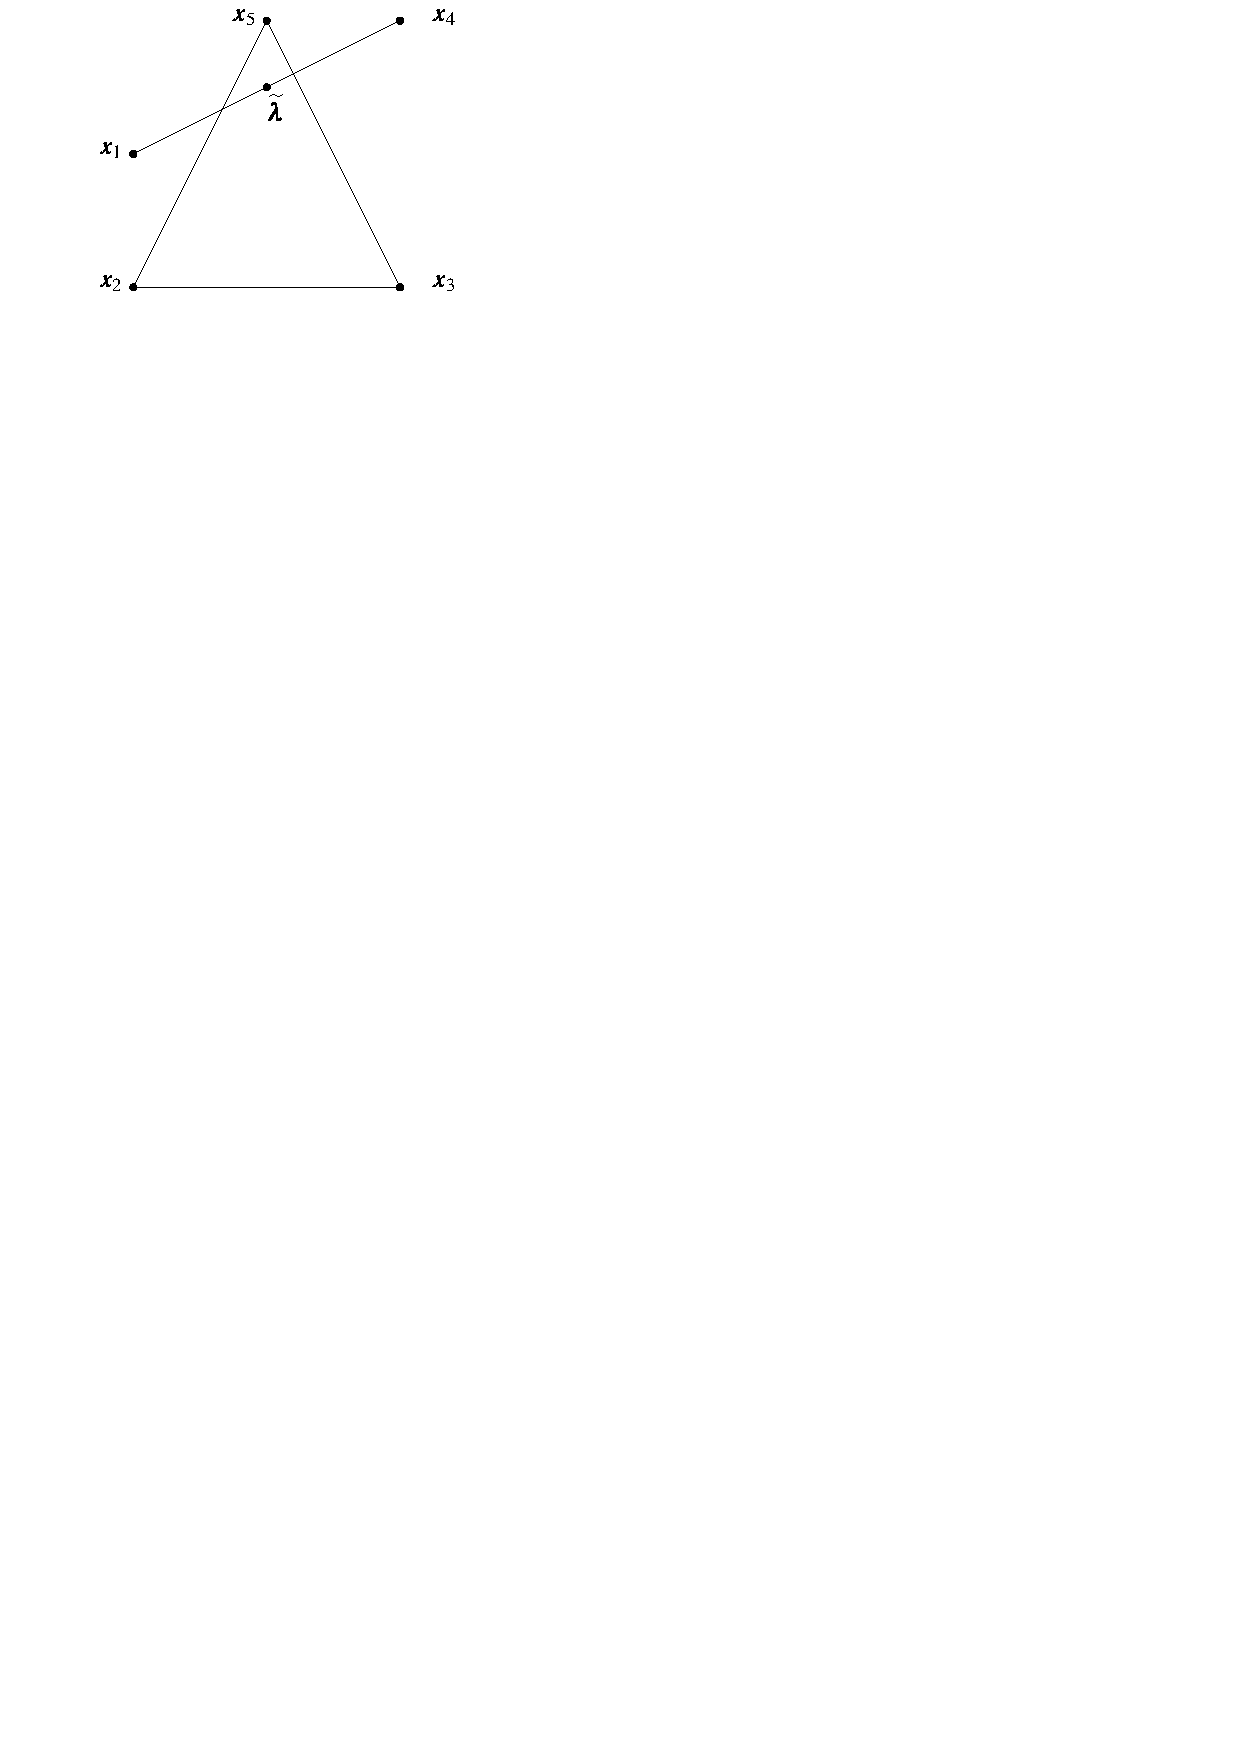
\includegraphics[page=1, width=.3\textwidth]{pictures.pdf}
            \end{figure}

        Further: \(\ve s=\sgn\ve\la=\usv+--+-\in\mc V(X)\); \(\card{\mc V(X)}=21\); and
            \begin{comment}
            \begin{align*}
                \mc V(X)
                    &=\left\{
                        \sv\ze+-+-, \sv+--+-,   \sv+-\ze+-, \snl
                        \sv+-+--,   \sv+-+-\ze, \sv+-+-+,   \snl
                        \sv+-+\ze-, \sv+-++-,   \sv+\ze-+-, \snl
                        \sv++-+-
                    \right\}
            \end{align*}
            \end{comment}
            \begin{align*}
                \mc C(X)
                    &=\left\{
                        \sv\ze+-+-,   \sv+-\ze+-,   \sv+-+-\ze, \snl
                        \sv+-+\ze-,   \sv+\ze-+-
                    \right\}.
            \end{align*}
            Note that \(\ve s\notin\mc C(X)\) since \(\ve t=\usv+-\ze+-\in\mc V(X)\) and \(\supp\ve t\varsubsetneq\supp\ve s\).  As for the dual sets, \(\card{\mc V^\perp(X)}=83\), and
            \begin{comment}
            \begin{align*}
                \mc V^*(X)
                    &=\left\{
                        \sv\ze\ze+++,  \sv\ze+---,    \sv\ze+\ze--,     \snl
                        \sv\ze++--,    \sv\ze++\ze-,  \sv\ze+++-,       \snl
                        \sv\ze+++\ze,  \sv\ze++++,    \sv+----,         \snl
                        \sv+---\ze,    \sv+---+,      \sv+--\ze+,       \snl
                        \sv+--++,      \sv+-\ze++,    \sv+-+++,         \snl
                        \sv+\ze---,    \sv+\ze--\ze,  \sv+\ze--+,       \snl
                        \sv+\ze-\ze+,  \sv+\ze-++,    \sv+\ze\ze++,     \snl
                        \sv+\ze+++,    \sv++---,      \sv++--\ze,       \snl
                        \sv++--+,      \sv++-\ze+,    \sv++-++,         \snl
                        \sv++\ze--,    \sv++\ze-\ze,  \sv++\ze-+,       \snl
                        \sv++\ze\ze+,  \sv++\ze++,    \sv+++--,         \snl
                        \sv+++-\ze,    \sv+++-+,      \sv+++\ze-,       \snl
                        \sv+++\ze\ze,  \sv+++\ze+,    \sv++++-,         \snl
                        \sv++++\ze,    \sv+++++
                    \right\}
            \end{align*}
            \end{comment}
            \begin{align*}
                \mc C^\perp(X)
                    &=\left\{
                        \sv\ze\ze+++,   \sv\ze+\ze--,   \sv\ze++\ze-,   \snl
                        \sv\ze+++\ze,   \sv+\ze--\ze,   \sv+\ze-\ze+,   \snl
                        \sv+\ze\ze++,   \sv++\ze-\ze,   \sv++\ze\ze+,   \snl
                        \sv+++\ze\ze
                    \right\}.
            \end{align*}
        \end{Example}

    \subsection{General Oriented Matroids}
        This section closely follows \cite[section 7.4]{ZieglerBook}.
        Before giving the definition of a general oriented matroid, three more definitions are needed for collections of sign vectors.
        \begin{Definition}  Let \(\ve s,\ve t,\ve u\) be sign vectors of length \(n\).
            \begin{enumerate}
                \item   The \dfn{composition} of  \(\ve s\) and \(\ve t\) is the sign vector \(\ve s\circ\ve t\) with coordinates
                        \begin{align*}
                            (\ve  s\circ\ve t)_i
                                =   \begin{cases}
                                        s_i     &   ,\text{ }s_i\ne0\\
                                        t_i     &   ,\text{ }s_i=0.
                                    \end{cases}
                        \end{align*}
                \item   The separation set of \(\ve s\) and \(\ve t\) is the set
                        \[
                            \sep{\ve s}{\ve t}
                                =   \setb{i\in\brac n}{s_i=-t_i\ne0}.
                        \]
                \item   If \(j\in\sep{\ve s}{\ve t}\), then \(\ve u\) \dfn{eliminates \(j\) between \(\ve s\) and \(\ve t\)} if \(u_j=0\) and for every \(i\notin\sep{\ve s}{\ve t}\), the equality \(u_i=(\ve s\circ\ve t)_i\) holds.
            \end{enumerate}
        \end{Definition}

        Notice that \(\sep{\ve s}{\ve t}=\sep{\ve t}{\ve s}\) and composition is not a commutative operation (Example \ref{Ex:OrientedOps}).  It is an associative operation since
            \begin{align*}
                (\ve s\circ(\ve t\circ\ve u))_i
                    =   ((\ve s\circ\ve t)\circ\ve u)_i
                    =   \begin{cases}
                            s_i     &,\text{ }s_i\ne0\\
                            t_i     &,\text{ }s_i=0\ne t_i\\
                            u_i     &,\text{ }s_i=0=t_i
                        \end{cases}.
            \end{align*}

        \begin{Example}\label{Ex:OrientedOps}
            Let \(\ve s=\usv+++0-\), and \(\ve t=\usv+-0++\).  Then
                \begin{itemize}
                    \item   \(\ve s\circ\ve t=\usv++++-\),
                    \item   \(\sep{\ve s}{\ve t}=\seta{2,5}\), and
                    \item   \(\ve u\) eliminates \(2\) between \(\ve s\) and \(\ve t\) if and only if \(\ve u\) is of the form \(\usv+0++\alpha\) for \(\alpha\in\seta{-,0,+}\).
                \end{itemize}

            On the other hand
                \begin{itemize}
                    \item   \(\ve t\circ\ve s=\usv+-+++\) and
                    \item   \(\ve u\) eliminates \(2\) between \(\ve t\) and \(\ve s\) if and only if \(\ve u\) is of the form \(=\usv+0++\beta\) for \(\beta\in\seta{-,0,+}\).
                \end{itemize}
        \end{Example}

        \begin{Definition}
            A set \(\mc V^\perp\sbset\seta{-,0,+}^n\) is the set of \dfn{covectors of an oriented matroid} if it satisfies the following:
                \begin{enumerate}
                    \item   \(\ve 0\in\mc V^\perp\);
                    \item   if \(\ve s\in\mc V^\perp\), then \(-\ve s\in\mc V^\perp\);
                    \item   if \(\ve s,\ve t\in\mc V^\perp\), then \(\ve s\circ\ve t\in\mc V^\perp\)
                    \item   if \(\ve s,\ve t\in\mc V^\perp\) and \(j\in\sep{\ve s}{\ve t}\), then there is some \(\ve u\in\mc V^\perp\) such that \(\ve u\) eliminates \(j\) between \(\ve s\) and \(\ve t\).
                \end{enumerate}
        \end{Definition}

        Covectors as described in section \ref{SSec:Realizable} satisfy the properties above, and therefore do form the set of covectors of an oriented matroid.


    \subsection{The Dual of an Oriented Matroid}
        For proofs of the results in this subsection, see either \cite{ZieglerBook} or \cite{OrientedMatBook}.

        Recall that the definition of orthogonality and dual were in terms of sign vectors.  Thus it makes sense to apply these operations to the covectors in a general oriented matroid.  In general, \((S^\perp)^\perp=S\).  Thus taking duals of a set leads to at most two distinct sets.  For \(\mc V^\perp\) the set of covectors of a general oriented matroid, define the \dfn{set of vectors} to be \(\mc V=(\mc V^\perp)^\perp\).  One can define circuits and cocircuits analogously.  Similar to the case of realizable oriented matroids, any of these four sets can be used to determine the others.

        A nontrivial result of oriented matroid theory is that the set of vectors of an oriented matroid is also the set of covectors of a different\footnote{As long as \(\mc V\ne\seta{\ve 0}\).  This follows since \(\mc V\cap\mc V^\perp=\seta{\ve 0}\).} oriented matroid.  This oriented matroid is called the \dfn{dual} of the original oriented matroid.

        In the case of a realizable oriented matroid (realized by the set of points \(V\)), the dual is also realizable, and is realized by a Gale diagram \(\Gamma\in\galed V\). 
     \chapter{Modifying Gale Diagrams}\label{chap:GaleDiagMod}

This chapter explores certain operations on Gale diagrams and how these operations affect the polytopes.



\section{Joins and Direct Sums}

Recall, from Sections \ref{SSec:Join} and \ref{SSec:DirectSum}, the definitions of join and direct sum for point sets.  If \(X=\seta{\ve p_1,\ve p_2\dc\ve p_n}\sbset\R{d_1}\) and \(Y=\seta{\ve q_1,\ve q_2\dc\ve q_m}\sbset\R{d_2}\), then
    \[
        X\join Y
            =
                \setb{\begin{bmatrix}\ve p_i\\\ve0_{d_2}\\-1\end{bmatrix}}{i\in\brac n}
                \cup
                \setb{\begin{bmatrix}\ve 0_{d_1}\\\ve q_j\\1\end{bmatrix}}{j\in\brac m}
            \sbset
                \R{d_1+d_2+1}
    \]
and
    \[
        X\oplus Y
            =
                \setb{\begin{bmatrix}\ve p_i\\\ve0_{d_2}\end{bmatrix}}{i\in\brac n}
                \cup
                \setb{\begin{bmatrix}\ve 0_{d_1}\\\ve q_j\end{bmatrix}}{j\in\brac m}
            \sbset
                \R{d_1+d_2}.
    \]
Since these operations are defined for general point sets, it makes sense to ask what happens if you perform them on two Gale diagrams.
\begin{Theorem}\label{Thm:DSumAndJoin}
    If \(P\) and \(Q\) are polytopes, \(\Gamma\in\galed(P)\), and \(\Lambda\in\galed(Q)\), then
        \[
            \Gamma\oplus \Lambda
                \in
                \galed(P\join Q)
        \]
    and
        \[
            \Gamma\join \Lambda
                \in
                \galed(P\oplus Q).
        \]
\end{Theorem}
\begin{proof}
    Suppose the following:
        \begin{align*}
            \dim P&=d_1;&
                \dim Q&=d_2;\\
            P&\sbset\R{d_1};&
                Q&\sbset\R{d_2};\\
            \vrt P&=\seta{\ve v_1,\ve v_2\dc\ve v_n};&
                \vrt Q&=\seta{\ve w_1,\ve w_2\dc\ve w_m};\\
            \ve 0_{d_1}&\in\relint P;&
                \ve 0_{d_2}&\in\relint Q;\\
            \dim\aff&\seta{\ve v_1,\ve v_2\dc\ve v_{d_1+1}}=d_1;&
                \dim\aff&\seta{\ve w_1,\ve w_2\dc\ve w_{d_2+1}}=d_2;
        \end{align*}
    and
        \begin{align*}
            \rref
                    \begin{bmatrix}
                        1       &   1       &   \cdots  &   1       \\
                        \ve v_1 &   \ve v_2 &   \cdots  &   \ve v_n
                    \end{bmatrix}
                        &=
                        \left[
                            \begin{array}{@{}c|c@{}}
                                I_{d_1+1} & A
                            \end{array}
                        \right]; &
                \rref
                    \begin{bmatrix}
                        1       &   1       &   \cdots  &   1       \\
                        \ve w_1 &   \ve w_2 &   \cdots  &   \ve w_m
                    \end{bmatrix}
                        &=
                        \left[
                            \begin{array}{@{}c|c@{}}
                                I_{d_2+1} & B
                            \end{array}
                        \right].
        \end{align*}
    Then order the vertices of \(P\join Q\) as follows:
        \begin{align*}
                \seta{
                \begin{bmatrix} \ve v_1\\       \ve 0_{d_2}\\   -1  \end{bmatrix}\dc
                \begin{bmatrix} \ve v_{d_1+1}\\ \ve 0_{d_2}\\   -1  \end{bmatrix},
                \begin{bmatrix} \ve 0_{d_1}\\   \ve w_1 \\      1   \end{bmatrix}\dc
                \begin{bmatrix} \ve 0_{d_1}\\   \ve w_{d_2+1}\\ 1   \end{bmatrix},
                \begin{bmatrix} \ve v_{d_1+2}\\ \ve 0_{d_2}\\   -1  \end{bmatrix}\dc
                \begin{bmatrix} \ve v_{n}\\     \ve 0_{d_2}\\   -1  \end{bmatrix},
                \begin{bmatrix} \ve 0_{d_1}\\   \ve w_{d_2+2}\\ 1   \end{bmatrix}\dc
                \begin{bmatrix} \ve 0_{d_1}\\   \ve w_{m}\\     1   \end{bmatrix}
                }.
        \end{align*}
    Here, the first \(d_1+d_2+2=\dim(P\join Q)+1\) vertices are affinely independent.  Now, use the techniques of Section \ref{SSec:ComputingGD} to compute a Gale transformation of \(P\join Q\) as follows:
    Form the matrix
        \begin{align*}
            Z=
            \left[
            \begin{array}{ccc|ccc|ccc|ccc}
                1               &\cdots  &1               &1               &\cdots  &1
                &1              &\cdots  &1               &1               &\cdots  &1   \\
                \ve v_1         &\cdots  &\ve v_{d_1+1}   &\ve 0_{d_1}     &\cdots  &\ve 0_{d_1}
                &\ve v_{d_1+2}  &\cdots  &\ve v_n         &\ve 0_{d_1}     &\cdots  &\ve 0_{d_1}     \\\hline
                \ve 0_{d_2}     &\cdots  &\ve 0_{d_2}     &\ve w_1         &\cdots  &\ve w_{d_2+1}
                &\ve 0_{d_2}    &\cdots  &\ve 0_{d_2}     &\ve w_{d_2+1}   &\cdots  &\ve w_m         \\
                -1              &\cdots  &-1              &1               &\cdots  &1
                &-1             &\cdots  &-1              &1               &\cdots  &1
            \end{array}
            \right].
        \end{align*}


    First, add the first row to the last row, and then perform, in the first \(d_1+1\) rows, the operations that transformation the matrix \(\left[\begin{array}{cccc}1&1&\cdots&1\\ \ve v_1&\ve v_2&\cdots&\ve v_n\end{array}\right]\) into \(\left[\begin{array}{@{}c|c@{}}I_{d_1+1} & A\end{array}\right]\).  Note that in the \(1,2\) and \(1,4\) blocks each column will be the same.  Call this common \((d_1+1)\)-dimensional vector \(\ve v\).  Further, denote an \(r\times s\) matrix with all entries \(0\) by \(\zmat rs\).  That is,
            \begin{comment}
            \rref\left[
                \begin{array}{ccc|ccc|ccc|ccc}
                    1               &\cdots     &1
                    &1              &\cdots     &1
                    &1              &\cdots     &1
                    &1              &\cdots     &1
                    \\
                    \ve v_1         &\cdots     &\ve v_{d_1+1}
                    &\ve0_{d_1}     &\cdots     &\ve0_{d_1}
                    &\ve v_{d_1+2}  &\cdots     &\ve v_n
                    &\ve0_{d_1}     &\cdots     &\ve0_{d_1}
                    \\  \hline
                    \ve 0_{d_2}     &\cdots     &\ve 0_{d_2}
                    &\ve w_1        &\cdots     &\ve w_{d_2+1}
                    &\ve0_{d_2}     &\cdots     &\ve 0_{d_2}
                    &\ve w_{d_2+2}  &\cdots     &\ve w_{m}
                    \\
                    -1              &\cdots     &-1
                    &1              &\cdots     &1
                    &-1             &\cdots     &-1
                    &1              &\cdots     &1
                \end{array}
            \right]\\
            \end{comment}
        \begin{align*}
            M&= \rref Z
                =
                \rref\left[
                    \begin{array}{c|c|c|c}
                        I_{d_1+1}
                            &\begin{array}{ccc}{\olay{\ve v}{\ve w_1}}&\cdots&{\olay{\ve v}{\ve w_{d_2+1}}}\end{array}
                            &A
                            &\begin{array}{ccc}\olay{\ve v}{\ve w_{d_2+2}}&\cdots&\olay{\ve v}{\ve w_m}\end{array}
                        \\ \hline
                        \zmat{d_2+1}{d_1+1}
                            &\begin{array}{ccc}\ve w_1&\cdots&\ve w_{d_2+1}\\ 2&\cdots&2\end{array}
                            &\zmat{d_2+1}{n-d_1+1}
                            &\begin{array}{ccc}\ve w_{d_2+2}&\cdots&\ve w_{m}\\ 2&\cdots&2\end{array}
                    \end{array}
                \right].
        \end{align*}

    Next, use the bottom row of the matrix to turn the \(1,2\) and \(1,4\) blocks into all zeros.  Then move the bottom row to the \((d_1+2)\)th row, divide it by \(2\) and shift each of the remaining rows down, that is:
        \begin{align*}
            M
                &=
                \rref\left[
                    \begin{array}{c|c|c|c}
                        I_{d_1+1}
                            &\zmat{d_1+1}{d_2+1}
                            &A
                            &\zmat{d_1+1}{m-d_2-1}
                        \\ \hline
                        \zmat{d_2+1}{d_1+1}
                            &\begin{array}{ccc}1&\cdots&1\\ \ve w_1&\cdots&\ve w_{d_2+1}\end{array}
                            &\zmat{d_2+1}{n-d_1+1}
                            &\begin{array}{ccc}1&\cdots&1\\ \ve w_{d_2+2}&\cdots&\ve w_{m}\end{array}
                    \end{array}
                \right].
        \end{align*}

    Now, in the bottom \(d_2+1\) rows, perform the row operations that transformation the matrix \(\left[\begin{array}{cccc}1&1&\cdots&1\\ \ve w_1&\ve w_2&\cdots&\ve w_m\end{array}\right]\) into \(\left[\begin{array}{@{}c|c@{}}I_{d_2+1} & B\end{array}\right]\).  Thus
        \begin{align*}
            M
                &=
                \left[
                    \begin{array}{c|c}
                        I_{d_1+d_2+2}
                            &\hspace{-5pt}\begin{array}{c|c}
                                A   &[0]\\
                                \hline
                                [0] &B
                             \end{array}
                    \end{array}\hspace{-5pt}
                \right]
        \end{align*}
    and so a Gale transformation of \(P\join Q\) is given by the multiset of the columns of the matrix
        \begin{align*}
            \left[
                \begin{array}{c|c|c|c}
                    -\Tr A  &[0]    &I      &[0]    \\ \hline
                    [0]     &-\Tr B &[0]    &I
                \end{array}
            \right].
        \end{align*}
    These are exactly the elements of \(\Gamma\oplus\Lambda\).

    The second result holds by oriented matroid duality.
\end{proof}


\subsection{\protect$d\protect$-Polytopes with \protect$d+2\protect$ Vertices}\label{SSec:dPlusTwo}
    As an application of Theorem \ref{Thm:DSumAndJoin}, all \(d\)-polytopes with \(d+2\) vertices are classified.  This section follows the discussion found in \cite{McMullenBook}.

    Let \(P\) be a \(d\)-polytope with \(d+2\) vertices, and let \(\Gamma\) be a standard Gale diagram of \(P\).  Since \(\Sp0=\seta{-1,1}\sbset\RR\), as a set \(\seta{-1,1}\sbset\Gamma\sbset\seta{-1,0,1}\).  Because \(\Gamma\) is a Gale diagram,
        \begin{align*}
            p
                &=  \card{\setb{\ve x\in\Gamma}{\ol{\ve x}=-1}}
                    \ge 2\\
            q
                &=  \card{\setb{\ve x\in\Gamma}{\ol{\ve x}=1}}
                    \ge 2.
        \end{align*}
    This leaves \(a=d+2-p-q\) points in \(\Gamma\), and they must all be at the origin.  A point at the origin in a Gale diagram corresponds to the apex of a pyramid in the polytope (Theorem \ref{Thm:GalePyr}).  Thus \(P\) is an \(a\)-fold pyramid over a polytope \(Q\) whose Gale diagram \(\Lambda\) has \(p\ge 2\) points on one side of the origin, and \(q\ge 2\) points on the other.

    The Gale diagram \(\Lambda\) is the join of the Gale diagrams of a \((p-1)\)-simplex and a \((q-1)\)-simplex.  Hence, by Theorem \ref{Thm:DSumAndJoin}, \(P\) is combinatorially equivalent to the polytope
        \[
            \pyr_a\left(\simp{p-1}\oplus\simp{q-1}\right).
        \]
    where \(a+p+q=d+2\) and \(p,q\ge 2\).

    Note that the combinatorial type of each \(d\)-polytope with \(d+2\) vertices can be specified by the unordered pair \((p,q)\).  So to count the number of combinatorial types of these polytopes, one only needs to count the number of such pairs.  Assume, without loss of generality, that \(p\le q\).  The pairs are then of the following form:
        \begin{align*}
            (2,q)
                &,\qquad 2\le q\le d\\
            (3,q)
                &,\qquad 3\le q\le d-1\\
                &\vdots\\
            \left(\floor{\frac d2},q\right)
                &,\qquad \floor{\frac d2}\le q\le\ceil{\frac d2}.
        \end{align*}

    Thus, if \(d\) is odd, then there are
        \begin{align*}
            2+4+\dotsb+(d-1)
                &=  2\left(1+2+\dotsb+\frac{d-1}2\right)
                =   \frac{d^2}4-\frac14
                =   \floor{\frac{d^2}4}
        \end{align*}
    combinatorial types of these polytopes.  If \(d\) is even, then there are
        \begin{align*}
            1+3+\dotsb+(d-1)
                &=  2+4+\dotsb+d-\frac d2
                =   \frac{d^2}4
                =   \floor{\frac{d^2}4}
        \end{align*}
    types of these polytopes.

    In \cite{McMullenBook}, the following lemma is proved.
    \begin{Lemma}
        Let \(\Gamma\) be a Gale diagram of a \(d\)-polytope \(P\) with \(n\) vertices.  Then \(P\) is a simplicial polytope if and only if for every hyperplane \(H\in\R{n-d-1}\) containing \(\ve 0\) the following holds:
            \[
                \ve 0
                    \notin \relint\conv(\Gamma\cap H).
            \]
    \end{Lemma}

    Combining this with the above discussion yields:
    \begin{Theorem}
        There are \(\floor{{d^2}/4}\) combinatorial types of \(d\)-polytopes with \(d+2\) vertices.  Furthermore, each of these polytopes is of the form \(\pyr_a\left(\simp{p-1}\oplus\simp{q-1}\right)\) where \(a+p+q=d+2\) and \(p,q\ge2\).  Moreover, \(\floor{d/2}\) of these polytopes are simplicial.
    \end{Theorem}

    \begin{comment}
    Thus, letting \(\Gamma(\simp{j})\) denote the standard Gale diagram of the \(j\)-simplex,
         \[
            \Gamma  =   \Gamma(\simp{k_{-1}-1})\join\Gamma(\simp{k_{1}-1}).
         \]
    Hence, by Theorem \ref{Thm:DSumAndJoin}, \(P\) is a direct sum of two simplices.
    \end{comment}

\section{Adding Points to Gale Diagrams}
    The first thing one should do in a section entitled ``Adding Points to Gale Diagrams" is discuss under what conditions adding a point to a Gale diagram yields a Gale diagram.  Thus, suppose \(\Gamma\in\galed(P)\) is a Gale diagram of some \(d\)-polytope \(P\) with \(n\) vertices, and let \(\ve x\in\R{n-d-1}\) be any point.  Then \(\Gamma\cup\seta{\ve x}\) is a Gale diagram of some \((d+1)\)-polytope with \(n+1\) vertices.  This is true since every hyperplane still has at least two points in both of its open half-spaces.  It should be clear that the location of the new point does matter in determining the new polytope.  Adding a point to a Gale diagram increases the number of points by \(1\), but not the dimension of the space in which the Gale diagram lies. Thus the dimension of the new polytope is \(1\) greater than the dimension of the old polytope.

    Points can be added to Gale diagrams in many ways.  Unfortunately, it is possible given two Gale diagrams  \(\Gamma,\Lambda\in\galed(P)\) to add a point to both \(\Gamma\) and \(\Lambda\) in the same way (such as adding a point antipodal to the point corresponding to a particular vertex), yet not have the two new polytopes be combinatorially equivalent.

    \subsection{Adding an Antipode to a Gale Diagram}
        \begin{figure}[p!hbt]
            \centering
                \includegraphics[width=.7\textwidth, page=16]{pictures.pdf}
            \caption{Two Gale diagrams of $\xp3$.\label{Fig:2GaleDXp3}}
        \end{figure}

        \begin{figure}[p!hbt]
            \centering
                \includegraphics[width=.8\textwidth, page=17]{pictures.pdf}
            \caption{Adding an antipode $\ol{1'}$ to the point $\ol{1}$ in a Gale diagram of $\xp3$. (cf.{} Figure \ref{Fig:AddPt2Gale2})\label{Fig:AddPt2Gale1}}
        \end{figure}

        \begin{figure}[p!hbt]
            \centering
                \includegraphics[width=.8\textwidth, page=18]{pictures.pdf}
            \caption{Adding an antipode $\ol{1'}$ to the point $\ol{1}$ in a Gale diagram of $\xp3$. (cf.{} Figure \ref{Fig:AddPt2Gale1})\label{Fig:AddPt2Gale2}}
        \end{figure}

        As an example; consider the crosspolytope \(\xp3\).  Figure \ref{Fig:2GaleDXp3} shows two consubstantial standard Gale diagrams for \(\xp3\).  If a point \(\ol{1'}\) is added that is antipodal to \(\ol 1\) in each of these Gale diagrams, then Figures \ref{Fig:AddPt2Gale1} and \ref{Fig:AddPt2Gale2} show the graphs of the polytopes with each of these Gale diagrams.  Let \(P\) be a polytope with the Gale diagram in Figure \ref{Fig:AddPt2Gale1}, and \(Q\) be a polytope with the Gale diagram in Figure \ref{Fig:AddPt2Gale2}.  Note that \(\conv\seta{2,5}\) is not an edge in \(P\), whereas in \(Q\) it is.  Hence, \(P\) and \(Q\) cannot be combinatorially equivalent.

        The facets of \(P\) are the \(3\)-dimensional pyramids \(23456\) and \(12345\) each with base \(2345\), as well as the following \(3\)-simplices.
            \begin{align*}
                &11'45&     &11'35&     &11'24&     &11'23\\
                &1'456&     &1'356&     &1'246&     &1'236
            \end{align*}
        The facets of \(Q\) are the triangular bipyramid \(23456\) with base \(256\), as well as the following \(3\)-simplices.
            \begin{align*}
                &11'45&     &11'35&     &11'24&     &11'23\\
                &1'456&     &1'356&     &1'246&     &1'236\\
                &1245&      &1235&      &&&
            \end{align*}
    \subsection{Duplicating a Point in a Gale Diagram}
        On the other hand, an operation that is well defined is that of adding a duplicate of an existing point to a Gale diagram.
        Let \(P\) be a \(d\)-polytope with vertex set \(\vrt P=\seta{\ve v_1,\ve v_2\dc\ve v_n}\).  Let \(\Gamma\) be a Gale diagram of \(P\), and let \(Q\) be a \((d+1)\)-polytope with vertex set \(\vrt Q=\seta{\ve w_{1'},\ve w_1,\ve w_2\dc\ve w_n}\) whose Gale diagram \(\Lambda\) satisfies \(\ol{\ve w}_{1'}=\ol{\ve v}_1\) and \(\ol{\ve w}_i=\ol{\ve v}_i\) otherwise.

        Let \(Y\) be a cofacet of \(Q\), that is, a minimal coface and consider the following four cases:
            \begin{enumerate}
                \item   (\(\seta{\ve w_1,\ve w_{1'}}\sbset Y\))  This case cannot happen since the set \(\ol{Y}\setminus\seta{\ol{\ve w}_1}\) captures the origin, and \(Y\setminus\seta{\ve w_1}\varsubsetneq Y\).
                \item   (\(\ve w_1\in Y\) and \(\ve w_{1'}\notin Y\))  For this case, let \(X=\setb{\ve v_i}{\ve w_i\in Y}\).  Then since \(\ol Y=\ol X\), the set \(Y\) is a cofacet if and only if \(X\) is a cofacet.
                \item   (\(\ve w_1\notin Y\) and \(\ve w_{1'}\in Y\))  Here, set \(X=\setb{\ve v_i}{\ve w_i\in Y\text{ or }i=1}\).  In this case, \(\ol Y=\ol X\) again, and so \(Y\) is a cofacet if and only if \(X\) is a cofacet.
                \item   (\(\seta{\ve w_1,\ve w_{1'}}\cap Y=\mt\)) For the final case, again set \(X=\setb{\ve v_i}{\ve w_i\in Y}\).  Once more, \(\ol Y=\ol X\), so that \(Y\) is a cofacet if and only if \(X\) is a cofacet.
            \end{enumerate}
        Thus the cofacets (and hence the facets) of \(Q\) are determined by the cofacets (and hence the cofacets) of \(P\) and vice versa. Geometrically, \(Q\) is combinatorially equivalent to a polytope with the following vertices:
            \begin{align*}
                \ve w_1
                    &=   \begin{bmatrix}\ve v_1\\1 \end{bmatrix}&
                \ve w_{1'}
                    &=   \begin{bmatrix}\ve v_1\\-1 \end{bmatrix}&
                \ve w_j
                    &=   \begin{bmatrix}\ve v_j\\0 \end{bmatrix},\,j\in\brac n\setminus\seta1
            \end{align*}
        Conceptually, first place \(P\) in \(\R{d+1}\).  Then the vertex \(\ve v_1\) is replaced by a line segment whose relative interior passes through \(\ve v_1\), and whose affine hull intersects that of the original polytope at precisely the point \(\ve v_1\).

        If \(P\) is a \(2\)-polytope with \(n\) vertices, then performing this operation at any vertex yields a polytope that is combinatorially equivalent to performing the operation at any other vertex.  The resulting polytope is combinatorially equivalent to the cyclic polytope \(\cyc{n+1}3\).  See Figure \ref{Fig:DupGale} for an example.  This process is called a \dfn{simplicial wedge} in \cite{SimplicialWedge}.

        \begin{figure}[p!hbt]
            \centering
                \includegraphics[width=.7\textwidth, page=32]{pictures.pdf}
            \caption{Duplicating the point\protect$\ol1\protect$ in a Gale diagram of \protect$\cyc25\protect$.\label{Fig:DupGale}}
        \end{figure} 
    \chapter{Gale Polytopes}
\label{chap:GalePolytopes}
Recall Gale's evenness condition, which exactly describes the facets of the cyclic polytope \(\cyc nd\) of dimension \(d\) with \(n\) vertices.
\begin{GEC}
    A subset \(S\sbset \brac n\) with \(\card S=d\) forms a facet of \(\cyc nd\) if and only if
        \[
            \card{\setb{k}{k\in S\text{ and }i<k<j}}\text{ is even for all } i<j,\, \seta{i,j}\cap S=\mt
        \]
\end{GEC}

It is reasonable to ask if a noncyclic polytope satisfies a weakened form of Gale's evenness condition, namely:
\begin{Definition}
    A \(d\)-polytope \(P\) with vertex set \(\vrt(P)=\seta{\ve v_1, \ve v_2\dc \ve v_n}\) is called a \dfn{Gale} polytope if there is an ordering of \(\vrt(P)\) such that each facet satisfies the following property:

    If \(S\sbset\brac n\) and \(F\) is a facet of \(P\) with \(\vrt(F)=\setb{\ve v_{s}}{s\in S}\), then
        \[
            \card{\setb{k}{k\in S\text{ and }i<k<j}}\text{ is even for all } i<j,\, \seta{i,j}\cap S=\mt.
        \]
\end{Definition}

An equivalent characterization is as follows:

Let \(P\) be a polytope,  \(\ve v_1, \ve v_2\dc\ve v_n\) be an ordering of \(\vrt(P)\) and \(S=\seta{\ve v_{i_1}, \ve v_{i_2}\dc \ve v_{i_k}}\sbset\vrt(P)\) be such that \(i_1<i_2<\dotsb<i_k\).  Then a \dfn{block} of \(S\) is a subset \(C\) of \(S\) such that if \(t=\min\setb{i_j}{\ve v_{i_j}\in C}\), then there is some \(r\in \N\) such that \(C=\seta{\ve v_t, \ve v_{t+1}\dc \ve v_{t+r-1}}\) and \(\ve v_{t+r}\notin S\).  In this case, the \dfn{length} of a block is \(\card{C}=r\).

\begin{Definition}
    A polytope \(P\) is \dfn{Gale} if there is an ordering of \(\vrt(P)\) such that if \(F\) is a facet of \(P\), then for each block \(G\) of \(\vrt F\)  one of the following holds:
        \begin{enumerate}
            \item   the length of \(G\) is even; or
            \item   \(\ve v_1\in G\); or
            \item   \(\ve v_n\in G\).
        \end{enumerate}
    Such an ordering of the vertices is called a \emph{Gale ordering}.  A block which contains \(\ve v_1\) is called an \dfn{initial block}.  A block which contains \(\ve v_n\) is called a \dfn{terminal block}.  A block which is neither initial, nor terminal is called \dfn{internal}.
\end{Definition}

In terms of blocks, a polytope is Gale if and only if there is an ordering of the vertices such that in each facet the only blocks of odd length are either initial, or terminal.  Note that a facet need not have either an initial block, or a terminal block.

An immediate consequence of either definition is:  If \(P\) is a Gale polytope with \(n\) vertices, and \(\ve v_1, \ve v_2\dc \ve v_n\) is a Gale ordering of \(\vrt(P)\), then so is \(\ve v_n, \ve v_{n-1}\dc \ve v_1\).  Note that all cyclic polytopes are Gale, and therefore all polytopes of dimension less than or equal to \(2\) are Gale.

\begin{Theorem}
    If \(P\) is a Gale polytope, then so is \(\pyr(P)\), a pyramid over \(P\).
\end{Theorem}
\begin{proof}
    Let \(\ve v_1, \ve v_2\dc\ve v_n\) be a Gale ordering of \(\vrt(P)\) and \(\ve w_1, \ve w_2\dc\ve w_{n+1}\) be the ordering of \(\vrt(\pyr(P))\) with \(\ve w_i\) corresponding to \(\ve v_i\) for \(i\in\brac n\), and with \(\ve w_{n+1}\) as the apex of the pyramid.

    Let \(F\) be a face of \(\pyr(P)\).  Then either \(\vrt(F)=\seta{\ve w_1,\ve w_2\dc\ve w_n}\), or \(\ve w_{n+1}\in \vrt(F)\).  In the first case, \(F\) contains only an initial block.

    In the second case, write \(\vrt(F)=\seta{\ve w_{i_1},\ve w_{i_2}\dc\ve w_{i_k},\ve w_{n+1}}\) with \(i_1<i_2<\dotsb<i_k<n+1\).  Then either \(i_k=n\), or \(i_k<n\).  If \(i_k=n\), then each block \(C\) of \(\seta{\ve w_{i_1},\ve w_{i_2}\dc\ve w_{i_k}}\) satisfies at least one of the following: \(C\) is internal of even length; \(C\) is initial; or \(\ve w_n\in C\).  Thus, after adding in \(\ve w_{n+1}\), each block \(C'\) satisfies one of the following respectively: \(C'\) is internal of even length; \(C'\) is initial; or \(C'\) is terminal.  In the case that\ \(i_k<n\), each block of \(\seta{\ve w_{i_1},\ve w_{i_2}\dc\ve w_{i_k}}\) is either initial, or is of even length.  Ergo, when \(\ve w_{n+1}\) is added the only change is that a terminal block of length \(1\) is added.
\end{proof}

\begin{Theorem}
    Suppose \(P\) is a Gale polytope, and let \(X\) be a collection of pairwise disjoint facets that each have an odd number of vertices.  Then \(\card X\le 2\) .
\end{Theorem}
\begin{proof}
    Let \(P\) be a Gale polytope, and \(F\) be a facet of \(P\) which has an odd number of vertices.

    Consider the blocks of \(F\). since \(F\) has an odd number of vertices, it must have either an initial or terminal block.  If this were not the case, then there would be an internal block with an odd number of vertices.
\end{proof}

\begin{Example}
    The above theorem shows that both the regular dodecahedron and regular icosahedron are not Gale polytopes.  The shaded facets in Figure \ref{Fig:RegDodeca} are all disjoint with an odd number of vertices, and there are more than two in each polytope.
    \begin{figure}[ht]
        \centering
            \includegraphics[width=.6\textwidth, page=24]{pictures.pdf}
        \caption{The regular dodecahedron and icosahedron are not Gale polytopes.\label{Fig:RegDodeca}}
    \end{figure}
\end{Example}

If \(P\) is a \(3\)-polytope with five or fewer vertices then it is combinatorially equivalent to one of \(\simp3\), \(\pyr(\cyc24)\), or \(\cyc35\) each of which is Gale.  However, there is a \(3\)-polytope with six vertices which is not Gale.  In order to demonstrate this, we will use Theorem \ref{Thm:SimpGale} which is a consequence of Lemma \ref{Thm:KleeMinty}.  For a proof, see \cite{KleeMinty}.
\begin{Lemma}[Klee, Minty 1972]\label{Thm:KleeMinty}
    Let \(X\) and \(Y\) be polytopes having the same number \(m\) of vertices, the vertices of \(X\) being \(\ve x_1,\ve x_2\dc\ve x_m\) and those of \(Y\) being \(\ve y_1,\ve y_2\dc\ve y_m\).  Suppose that for each index set \(I\sbset\brac m\),
        \[
            \conv\setb{\ve x_i}{i\in I}\text{ is a facet of }X
                \text{ implies }
                    \conv\setb{\ve y_i}{i\in I}\text{ is a facet of }Y.
        \]
    Then the reverse implications hold, whence \(X\) and \(Y\) are combinatorially equivalent.
\end{Lemma}

The following theorem is found in \cite{BayerBisz}.

\begin{Theorem}\label{Thm:SimpGale}
    If \(P\) is a simplicial Gale polytope, then \(P\) is a cyclic polytope.
\end{Theorem}
\begin{proof}
    First, recall that if \(\vrt(\cyc nd)=\seta{\ve v_1,\ve v_2\dc\ve v_n}\), then the set facets of \(\cyc{n}d\) is
        \[
            X=\setb{\conv\seta{\ve v_{i_1},\ve v_{i_2}\dc\ve v_{i_{d+1}}}}{\seta{\ve v_{i_1},\ve v_{i_2}\dc\ve v_{i_{d+1}}}\text{ satisfies Gale's evenness condition}}.
        \]

    Let \(P\) be a simplicial Gale polytope of dimension \(d\) with \(\card{\vrt{P}}=n\).  Then there is some ordering \(\ve w_1, \ve w_2\dc\ve w_n\) of \(\vrt P\) such that if \(\conv\seta{\ve w_1,\ve w_2\dc\ve w_{i_{d}}}\) is a facet of \(P\), then the set \(\conv\seta{\ve v_{i_1},\ve v_{i_2}\dc\ve v_{i_{d}}}\) is a facet of \(\cyc nd\) since the set of facets of \(\cyc nd\) is \(X\).

    Thus \(P\) and \(\cyc nd\) satisfy the hypothesis of Lemma \ref{Thm:KleeMinty}.  Hence \(P\) is combinatorially equivalent to \(\cyc nd\).
\end{proof}
\begin{comment}
\begin{proof}
    Thus, the map \(\ve w_i\mapsto\ve v_i\) induces a map \(\varphi\colon\fl P\rightarrow\fl{\cyc nd}\) from the face lattice of \(P\) to that of \(\cyc nd\) which is an injection.

    Suppose \(F=\conv\seta{\ve v_{i_1},\ve v_{i_2}\dc\ve v_{i_{d+1}}}\) is a facet of \(\cyc nd\) such that \(\varphi\nv F\)
    %=\conv\seta{\ve w_{i_1},\ve w_{i_2}\dc\ve w_{i_{d+1}}}
    is not a facet of \(P\).  Let \(F'\) be any facet of \(P\).  Then there is a sequence \(F=F_1,F_2\dc F_r=\varphi F'\) of facets of \(\cyc nd\) such that \(\card{\vrt(F_i)\cap\vrt(F_{i+1})}=d-1\) for each \(i\in\brac{r-1}\).  Thus, there is some \(t\) such that \(\varphi\nv F_1,\varphi\nv F_2\dc\varphi\nv F_t\) are not facets of \(P\), but \(\varphi\nv F_{t+1}\) is.

    Let \(R=F_t\cap F_{t+1}\).  Then \(R\in\fl{\cyc nd}\) since \(\fl{\cyc nd}\) is a lattice, and \(\varphi\nv R\in\fl{P}\) since \(P\) is simplicial and \(\varphi\nv R\sbset\varphi\nv F_t\in\fl P\).

    Since \(P\) is a polytope, there is some \(K\in\fl P\) such that \(\varphi\nv R\varsubsetneq K\varsubsetneq P\) with \(K\ne \varphi\nv F_{t+1}\)  \cite[page 57]{ZieglerBook}.  Similarly, if \(L\in\fl{\cyc nd}\) such that \(R\varsubsetneq L\varsubsetneq \cyc nd\), then either \(L=F_t\), or \(L=F_{t+1}\).  Since \(\varphi\) is an injection, it must be the case that \(\varphi K= F_t\).  Thus \(\varphi\) is an isomorphism, and \(P\) is cyclic.
\end{proof}
\end{comment}

Thus, for example, \(\xp3\) is not a Gale polytope since each vertex of \(\xp3\) lies on four edges, whereas \(\cyc36\) has two vertices which each lie on only three edges.

Since simplices are cyclic polytopes, and cyclic polytopes are simplicial, each facet of a cyclic polytope satisfies Gale's evenness condition.  However, this need not happen for a general Gale polytope.  The following is an example of a Gale polytope with a facet which is not Gale.

\begin{Example}
    Consider the \(5\)-dimensional cyclic polytope with vertices \(\ve x_1,\ve x_2,\ve x_3,\ve x_4,\ve x_5,\ve x_6,\ve x_7\).  Let \(P\) be a vertex figure of \(\cyc75\) at \(\ve x_4\).  Then \(P\) is a \(4\)-dimensional simplicial polytope with \(6\) vertices \(\ve z_1,\ve z_2,\ve z_3,\ve z_5,\ve z_6,\ve z_7\) (where \(\ve z_i\) corresponds to the edge \(\ve x_4\ve x_i\)).

    The facets of \(P\) are the convex hulls of the following sets:
        \begin{align*}
            \seta{\ve z_1, \ve z_2, \ve z_3, \ve z_5}&&
            \seta{\ve z_1, \ve z_2, \ve z_3, \ve z_7}&&
            \seta{\ve z_1, \ve z_2, \ve z_5, \ve z_7}&&
            \seta{\ve z_1, \ve z_3, \ve z_5, \ve z_6}&\\
            \seta{\ve z_1, \ve z_3, \ve z_6, \ve z_7}&&
            \seta{\ve z_1, \ve z_5, \ve z_6, \ve z_7}&&
            \seta{\ve z_2, \ve z_3, \ve z_5, \ve z_7}&&
            \seta{\ve z_3, \ve z_5, \ve z_6, \ve z_7}&.
        \end{align*}

    Let \(Q\) be a pyramid over \(P\) with apex \(\ve a\).  Then \(Q\) is a Gale polytope with Gale ordering
        \[
            \ve z_1,\ve z_2,\ve z_3,\ve a,\ve z_5,\ve z_6,\ve z_7.
        \]
    However, \(P\) (which is the base of the pyramid \(Q\), and therefore also a facet of \(Q\)) is not Gale since it is a simplicial \(4\)-polytope whose graph is not complete (it is missing the edge \(\conv\seta{\ve z_2,\ve z_6}\)) and therefore \(P\) is not cyclic.

    Notice that this construction generalizes to give infinitely many polytopes with this property.  Consider the cyclic polytope \(\cyc{2n+1}d\) (of dimension at least \(4\)) with an odd number of vertices.  Let \(P\) be a vertex figure of \(\cyc{2n+1}d\) at the vertex \(n+1\), and \(Q\) be a pyramid over \(Q\).
\end{Example}

\begin{Theorem}\label{Thm:GaleProduct}
    If \(P\) is a Gale \(d\)-polytope, and \(Q\) is a Gale \(d'\)-polytope, then \(P\times Q\) is a Gale \((d+d')\)-polytope.
\end{Theorem}

\begin{proof}
Suppose \(\ve v_1,\ve v_2\dc \ve v_n\) is a Gale ordering of \(\vrt(P)\), and \(\ve w_0,\ve w_1\dc \ve w_m\) is a Gale ordering of \(\vrt Q\).  Then define an ordering of \(\vrt(P\times Q)\) as follows:

Let \((V_1,\ve w_i)\) and \((V_{-1},\ve w_i)\) respectively be the sequences:
    \begin{align*}
        &(\ve v_1,\ve w_i),(\ve v_2,\ve w_i)\dc(\ve v_n,\ve w_i)\\
        &(\ve v_n,\ve w_i),(\ve v_{n-1},\ve w_i)\dc(\ve v_1,\ve w_i).
    \end{align*}
Define similarly, \((B_1,\ve w_i)\) and \((B_{-1},\ve w_i)\) for \(B\) a set of vertices of \(P\).

Claim: \((V_1,\ve w_0),(V_{-1},\ve w_1)\dc(V_{(-1)^m},\ve w_m)\) is a Gale ordering of \(P\times Q\).

First, consider the facets of \(P\times Q\) of the form \(P\times G\) where \(G\) is a facet of \(Q\).  The vertex \(\ve w_j\) is a vertex of \(G\) if and only if \((\ve v_i, \ve w_j)\) is a vertex of the facet \(P\times G\) for each \(\ve v_i\in\vrt(P)\).  In particular, the sequence \((V_{(-1)^j},\ve w_j)\) is part of a block of \(P\times G\).

If \(n\) is even, then each of these parts is of even length, and hence every block of \(P\times G\) is even.  If \(n\) is odd, then consider the blocks of \(G\).  If \(G\) has an initial block \(\ve w_0,\ve w_1\dc \ve w_t\), then \(P\times G\) has initial block \((V_1,\ve w_0),(V_{-1},\ve w_1)\dc (V_{(-1)^t},\ve w_t)\) (since \((\ve v_1,\ve w_{t+1})\) is not a vertex of \(P\times G\)).  A similar statement applies for terminal blocks.

Suppose that \(G\) has an internal block \(\ve v_k,\ve v_{k+1}\dc\ve v_{k+s-1}\).  Since this is an internal block, \(s\) must be even.  Thus the sequence \((V_{(-1)^k},\ve w_k),(V_{(-1)^{k+1}},\ve w_{k+1})\dc(V_{(-1)^{k+s-1}},\ve w_{k+s-1})\) is an internal block of \(P\times G\) of length \(\card{\vrt(P)}\cdot s\) (this is an even number).  This follows since each element of the above sequence is a vertex of \(P\times G\), and none of the vertices
    \[
        (\ve v_1,\ve w_{k-1}), (\ve v_n,\ve w_{k-1}), (\ve v_n,\ve w_{k+s}), (\ve v_1,\ve w_{k+s})
    \]
is a vertex of \(P\times G\).

Now, consider the facets of \(P\times Q\) of the form \(F\times Q\) with \(F\) a facet of \(P\).  In this case, similar to above, \(\ve v_i\in F\) if and only if \((\ve v_i,\ve w_j)\in F\times Q\) for each \(j\in\brac m\cup\seta0\).  The sequence \(B=\ve v_i,\ve v_{i+1}\dc\ve v_{i+k-1}\) is part of a block of \(F\) if and only if
    \begin{align*}
        \begin{cases}
            (B_1,\ve w_j)=
                (\ve v_i,\ve w_j),(\ve v_{i+1},w_j)\dc (\ve v_{i+k-1},\ve w_j)
                    &   ,j\text{ even}\\
            (B_{-1},\ve w_j)=
                (\ve v_{i+k-1},\ve w_j),(\ve v_{i+k-2},w_j)\dc(\ve v_i,\ve w_j)
                    &   ,j\text{ odd}\\
        \end{cases}
    \end{align*}
is part of a block of \(F\times Q\).  If \(B\) is an internal block of \(F\), then the above are internal blocks of \(F\times Q\).

Suppose that \(B\) is an initial block of \(F\) (in particular, \(i=1\), and \(B\) has length \(k\)).  Then:
    \begin{itemize}
        \item   \((B_1,\ve w_1)\) is an initial block of \(F\times Q\);
        \item   if \(m\) is odd, then \((B_{-1},\ve w_m)\) is a terminal block of \(F\times Q\);
        \item   if \(m\) is even, then \((B_{-1},\ve w_{m-1}),(B_1,\ve w_m)\) is an internal block of length \(2k\).
    \end{itemize}
Further, \((B_{-1},\ve w_{2\ell-1}),(B_1,\ve w_{2\ell})\) is an internal block of length \(2k\) for \(\ell\in\brac{\floor{m/2}}\).

The case that \(B\) is a terminal block is handled similarly.
\end{proof} 
    \chapter{Anticliques in Graphs of Polytopes}
\label{chap:Anticliques}

Let \(G=(V, E)\) be a graph.  An \dfn{anticlique} is a subset \(A\) of \(V\) (of cardinality at least \(2\)) such that \(E\cap\binom A2=\mt\).  If \(\card A=k\), then \(A\) is said to be a \(k\)-anticlique.  A \(2\)-anticlique is simply a nonedge.

Recall that if \(G\) is the graph of a \(d\)-polytope \(P\) with \(n\) vertices, and \(\Gamma\in\galed(P)\) is a Gale diagram of \(P\), then \(\seta{{\ve v}_i,{\ve v}_j}\) is a nonedge of \(P\) if and only if there is some hyperplane \(H_{i,j}\sbset\R{n-d-1}\) containing \(\ve0\) such that \(H_{i,j}^{(+)}\cap\Gamma=\seta{\ol{\ve v}_i,\ol{\ve v}_j}\).  Such a hyperplane is called a \dfn{separating} hyperplane.  The normal vector to \(H_{i,j}\) which has positive inner product with \(\ol{\ve v}_i,\ol{\ve v}_j\) and norm \(1\) is denoted \(\ve x_{i,j}\).

If \(P\) is a \(d\)-polytope with \(d+k\) vertices, then Theorem \ref{Thm:ConnectivityOfGraph} in Section \ref{Sec:GraphsOfPolytopes} implies that each vertex of \(\gr P\) must have degree at least \(d\).  If a graph \(H\) with \(d+k\) vertices has a \((k+1)\)-anticlique, then each vertex in the anticlique has degree at most \(d-1\), and hence \(H\) is not \(d\)-realizable.  However, the graph \(\left(\brac{d+k},\binom{\brac{d+k}}2\setminus\binom{\brac k}2\right)\) is \(d\)-connected, and furthermore has a \(K_{d+1}\) minor (the induced subgraph on the vertex set \(\seta{k, k+1\dc k+d}\) is complete) and thus \emph{could} be the graph of a \(d\)-polytope.  It will be shown that this cannot happen.  More precisely for \(k\ge 2\), let
    \[
        f(d,k)=\max\setb{n}{\text{there is some \(d\)-polytope \(P\) with \(d+k\) vertices and an \(n\)-anticlique}}.
    \]
Then the goal is to show that \(f(d,k)<k\) for \(k>2\).

\section{An Upper Bound on \protect$f\protect$}
First note that \(f\) is weakly increasing in both arguments.

\begin{Theorem}\ph
    \begin{enumerate}
        \item   \(f(d,k)\le f(d+1,k)\)
        \item   \(f(d,k)\le f(d,k+1)\)
    \end{enumerate}
\end{Theorem}
\begin{proof}
    Let \(P\) be a \(d\)-polytope with \(d+k\) vertices, and an \(f(d,k)\)-anticlique.
        \begin{enumerate}
            \item   The \((d+1)\)-polytope \(\pyr(P)\) has \((d+k)+1=(d+1)+k\) vertices and an \(f(d,k)\)-anticlique.
            \item   Let \(F\) be any facet of \(P\).  The \(d\)-polytope \(K(P;F)\) (defined in section \ref{Subsec:Kleetopes}) has \(d+(k+1)\) vertices and an \(f(d,k)\)-anticlique.
        \end{enumerate}
\end{proof}



Recall that a standard Gale diagram is one in which each point is either on the unit sphere, or at the origin.  Further if a point in the Gale diagram is at the origin, then the polytope is a pyramid with apex the corresponding point.  Since the main question is concerned with sizes of anticliques, and the anticliques of a pyramid are exactly those of its base, nothing is lost or gained in the assumption that a polytope is not a pyramid.

\begin{Theorem}\label{Thm:TrivialitiesAnticliques}
    Let \(P\) be a \(d\)-polytope with vertex set \(\seta{\ve v_1,\ve v_2\dc\ve v_{n}}\);  \(A=\seta{i_1,i_2\dc i_k}\sbset\brac n\); \(\setb{\ve v_{i}}{i\in A}\) be an anticlique;  \(\Gamma\) be a standard Gale diagram of \(P\); and \(\seta{i,j}\sbset A\).  Then
        \begin{enumerate}
            \item   \(\ol{\ve v}_i\ne\ve 0\).
            \item   \(\ol{\ve v}_i\ne-\ol{\ve v}_j\).
        \end{enumerate}
    Furthermore if \(k\ge3\), then
        \begin{enumerate}[resume]
            \item\label{ThmPt:notequal}   if \(\ol{\ve v}_i=\ol{\ve v}_j\) , then \(i=j\).
        \end{enumerate}
\end{Theorem}
\begin{proof}\ph
    \begin{enumerate}
        \item   If \(\ol{\ve v}_i=\ve 0\), then \(\conv\seta{\ve v_i,\ve v_t}\) is a face of \(P\) for each \(t\in\brac n\setminus\{i\}\).  In particular, \(\conv\seta{\ve v_i,\ve v_j}\) is an edge of \(G(P)\).
        \item  If \(\ol{\ve v}_i=-\ol{\ve v}_j\),and \(H_{i,j}\) is a separating hyperplane for \(\ol{\ve v}_i,\ol{\ve v}_j\) with normal vector \(\ve x_{i,j}\), then
                \[
                    0<\ip{\ve x_{i,j}}{\ol{\ve v}_i}=-\ip{\ve x_{i,j}}{\ol{\ve v}_j}<0.
                \]
        \item  Let \(H_{a,b}\) be a separating hyperplane for \(\ol{\ve v}_a,\ol{\ve v}_b\) with normal \(\ve x_{a,b}\) for each pair \(a,b\in A\).  Suppose \(\ol{\ve v}_i=\ol{\ve v}_j\) with \(i\ne j\).  Then for \(r\in A\setminus\seta{i,j}\),
                \[
                    0   <\ip{\ve x_{j,r}}{\ol{\ve v}_j}
                        =\ip{\ve x_{j,r}}{\ol{\ve v}_i}
                        \le 0.
                \]
            Hence \(i=j\).\qedhere
    \end{enumerate}
\end{proof}
\begin{Theorem}
    \(f(d,2)=2\)
\end{Theorem}
\begin{proof}
    If \(P\) is a \(d\)-polytope with \(d+2\) vertices, then \(P\) has a \(1\)-dimensional Gale diagram.  Since a nonedge requires that there be a separating hyperplane, and in this case there is only one possible hyperplane (namely the origin), each vertex can have at most one nonneighbor.  This implies that \(f(d,2)\le2\).  The polytope \(\pyr_{d-2}(\xp2)\) is \(d\)-dimensional with \(d+2\) vertices and a \(2\)-anticlique.  Thus \(f(d,2)=2\).
\end{proof}
\begin{Theorem}
    \(f(d,3)<3\)
\end{Theorem}
\begin{proof}
    Let \(P\) be a \(d\)-polytope with \(d+3\) vertices, and let \(\Gamma\) be  a standard Gale diagram of \(P\).  Suppose that \(P\) has a \(3\)-anticlique \(\seta{\ve v_1,\ve v_2,\ve v_3}\), and let \(\ve v_4\) be any other vertex of \(P\).  Note that since \(\Gamma\sbset\Sp1\) (assuming again that \(P\) is not  a pyramid), by writing each \(\ol{\ve v}_i\in\Gamma\) in polar coordinates only the angle \(\varphi_i\in[0,2\pi)\) is necessary to specify \(\ol{\ve v}_i\).  By Theorem \ref{Thm:TrivialitiesAnticliques} part \ref{ThmPt:notequal}, none of \(\varphi_1,\varphi_2,\varphi_3\) are equal, so assume \(\varphi_1<\varphi_2<\varphi_3\).  Further, if \(\varphi_1>0\), then rotating each point in \(\Gamma\) clockwise by an angle of \(\varphi_1\) produces a consubstantial standard Gale diagram, so assume
        \[
            0=\varphi_1<\varphi_2<\varphi_3<2\pi.
        \]

        \begin{center}
            \begin{figure}[h!bt]
                \includegraphics[page=23, width=.3\textwidth]{pictures.pdf}
            \end{figure}
        \end{center}

    Since \(\ve v_1\ve v_2\) is not an edge of \(P\), there is some hyperplane \(H_3\) through the origin such that \(H_3^{(+)}\cap\Gamma=\seta{\ol{\ve v}_1,\ol{\ve v}_2}\).  Therefore, \(\varphi_4\notin[0,\varphi_2]\).  Similarly, \(\varphi_4\notin[\varphi_2,\varphi_3]\), and \(\varphi_4\notin[\varphi_3,2\pi)\).  Since \(\Gamma\) is a standard Gale diagram, this means that \(\ol{\ve v}_4=\ve0\).  But this contradicts the assumption that \(P\) is not a pyramid.
\end{proof}


\begin{Lemma}\label{Lem:LocalCone}
    If
        \begin{itemize}
            \item   \(P\) is a \(d\)-polytope with vertex set \(V\cup Y\) of cardinality \(d+k\),
            \item   \(\card V=d\) and \(\card Y=k\),
            \item   \(Y\) is an anticlique of \(\gr P\), and
            \item   \(\ve v\in V\), then
        \end{itemize}
    \(\ve v\ve y\) is an edge of \(\gr P\) for each \(y\in Y\).
\end{Lemma}
\begin{proof}
    Let \(\ve v\in V\), \(\ve y\in Y\).  Since \(P\) is a \(d\)-polytope, it is \(d\)-connected, therefore each vertex of \(G(P)\) is adjacent to at least \(d\) other vertices.  But since \(Y\) is an anticlique, \(\ve y\) is adjacent to at most \(d\) other vertices. Hence \(\ve y\) is adjacent to exactly \(d\) other vertices, and since none of these other vertices is in \(Y\), \(\ve v\ve y\) is an edge of \(G(P)\).
\end{proof}

    The following is a general fact about polytopes.  A proof is included for completeness, but
\begin{Lemma}\label{Lem:LocallySimple}
    Let \(P\) be a \(d\)-polytope, \(\ve y\in\vrt P\) with \(\deg\ve y=d\), and \(V=N(\ve y)=\seta{\ve v_1,\ve v_2\dc\ve v_d}\).  Then for each subset \(X\) of \(V\) with cardinality \(d-1\) there is a unique facet \(F\) of \(P\) with \(X\sbset\vrt F\).
\end{Lemma}
\begin{proof}
    Each vertex of \(P\) lies in at least \(d\) facets since \(P\) is a \(d\)-polytope.  Let \(F\) be a facet containing \(\ve y\).  Since \(F\) is a \((d-1)\)-polytope, each vertex of \(G(F)\) has degree at least \(d-1\).  Thus \(\ve y\) must have either \(d-1\) or \(d\) neighbors in \(F\).  If \(\ve y\) had each of its \(d\) neighbors in \(F\), then \(\ve y\) would only lie in one facet.  Thus each facet in which \(\ve y\) lies contains exactly \(d-1\) neighbors of \(\ve y\).  Further, each element of \(\binom V{d-1}\) determines a unique facet of \(P\) since \(\ve y\) lies in at least \(d\) facets.
\end{proof}

Notice that this argument also shows that the set \(V\) above is affinely independent, and that \(V\) is not contained in any proper face of \(P\).

\begin{Theorem}\label{Thm:Anticliques}
    If \(k>2\), then \(f(d,k)<k\).
\end{Theorem}
\begin{proof}
    Proceed by induction on \(d\).  For the base case: the graph of a \(2\)-polytope with \(n\) vertices is a cycle of length \(n\), so a maximal anticlique can be obtained by taking every other vertex. Therefore \(f(2,k)=1+\floor{k/2}<k\).  Thus, suppose  for some \(d\) that \(f(d-1,k)<k\) for all \(k>2\).  The proof of the contrapositive will be shown, that is, if \(f(d,k)=k\), then \(k=2\).

    Let \(P\) be a \(d\)-polytope with \(d+k\) vertices and, without loss of generality, suppose that \(P\) is not a pyramid.  Suppose further, that \(P\) has a \(k\)-anticlique \(Y=\seta{\ve y_1,\ve y_2\dc\ve y_k}\).  Write \(\vrt(P)=\seta{\ve v_1,\ve v_2\dc\ve v_d}\cup Y\), let \(V=\seta{\ve v_1,\ve v_2\dc\ve v_d}\), and \(V_i=V\setminus\seta{\ve v_i}\) for \(i\in\brac d\).  Fix some \(i\in\brac d\), and for each \(j\in\brac k\), let \(F_{i,j}\) be the facet of \(P\) which contains \(V_i\cup\seta{\ve y_j}\) (Lemmata \ref{Lem:LocalCone} and \ref{Lem:LocallySimple}), and \(G_i\) be the smallest face of \(P\) which contains \(V_i\).

    Notice that \(G_i\sbset F_{i,j}\) for each \(j\in\brac k\), and that \(G_i\) is either a facet or a ridge since \(V\) is an affinely independent set.

        \begin{enumerate}
            \item   (\(G_i\) is a facet.)  In this case, for each \(j\in\brac k\), \(G_i=F_{i,j}=\conv(Y\cup V_i)\).  Thus \(P\) is a pyramid over \(G_i\) with apex \(\ve v_i\).  This is a contradiction.
            \item   (\(G_i\) is a ridge.)  Let \(F_1,F_2\) be the facets containing \(G_i\).  In this case, \(Y\) can be partitioned into two nonempty sets
                    \begin{align*}
                        Y_1 &=  \seta{\ve y_{a_1},\ve y_{a_2}\dc\ve y_{a_r}}&
                        Y_2 &=  \seta{\ve y_{b_1},\ve y_{b_2}\dc\ve y_{b_s}}&
                    \end{align*}
                such that
                    \begin{align*}
                        Y_1 &\sbset F_{i,a_1}   =   F_1&
                        Y_2 &\sbset F_{i,b_1}   =   F_2.&
                    \end{align*}

                If \(\card{Y_1}=2\), then \(F_1\) is a \((d-1)\)-polytope with \((d-1)+2\) vertices and \(G_i\) is a facet of \(F_1\).  Thus a Gale diagram of \(F_1\) is one dimensional with \(d+1\) vertices, and both \(\ol{\ve y}_{a_1}\) and \(\ol{\ve y}_{a_2}\) are on the same side of the origin.  However, \(\ve 0\in\relint\conv{\left(\ol{\vrt(F_1)\setminus Y_1}\right)}\).  Similarly, \(\card{Y_2}\ne2\).

                If \(\card{Y_1}\ge 3\), then \(F_{i,a_1}\) is a \((d-1)\)-polytope with \((d-1)+\card{Y_1}\) vertices, and a \(\card{Y_1}\)-anticlique, that is, \(f(d-1,\card{Y_1})\ge\card{Y_1}\).  This contradicts the inductive hypothesis.

                Hence \(\card{Y_1}=\card{Y_2}=1\), whence \(P\) is a \(d\)-polytope with \(d+2\) vertices and a \(2\)-anticlique.  Thence \(k=2\).
        \end{enumerate}
\end{proof}

\section{A Lower Bound on \protect$f\protect$}

\begin{Lemma}
    If
        \begin{itemize}
            \item   \(P\) is a \(d\)-polytope with \(d+k\) vertices,
            \item   \(\ve v\) is a vertex of \(P\) such that each facet containing \(\ve v\) is a simplex, and
            \item   \(\ve v\) is contained in a \(q\)-anticlique of \(P\), then
        \end{itemize}
    \(f(d,k+i)\ge q+i-1\) for \(i\in\brac d\).
\end{Lemma}
    For example, such a vertex exists when \(P\) is a simplex (in which case each vertex has this property) or if \(P\) is of the form \(P=K(P';F)\) where \(F\) is a facet of \(P'\) which is a simplex, so the Lemma is not vacuous.
\begin{proof}
    Let \(F_1,F_2\dc F_d\) be facets of \(P\) containing \(\ve v\), and set
        \begin{align*}
            P_0(\ve v)
                    &=P\\
            P_i(\ve v)
                    &=K(P;F_1,F_2\dc F_i)\\
            \seta{\ve v_i}
                    &=\vrt(P_i(\ve v))\setminus\vrt(P_{i-1}(\ve v)).
        \end{align*}
    Further, let \(A'\) be a \(q\)-anticlique of \(P\) which contains \(\ve v\), and set \(A=A'\setminus\seta{\ve v}\).

    For a fixed \(i\in\brac d\), the inclusion \(N(\ve v_i)\sbset N(\ve v)\cup\seta{\ve v}\) in \(\gr{P_i(\ve v)}\) implies that  \(A\cup\seta{\ve v_1,\ve v_2\dc\ve v_i}\) is a \((q-i-1)\)-anticlique in \(\gr{P_i(\ve v)}\).
\end{proof}

\begin{Theorem}\label{Thm:Bounds}
    If \(k,d>2\), then \(\ds k-1-\floor{\frac{k-3}d}\le f(d,k)\le k-1\).
\end{Theorem}
\begin{proof}
    Fix \(d>2\) and set \(t=\floor{(k-3)/d}\) and let \(Q_0=K(\simp d;F)\) for some facet \(F\) of \(\simp d\).  Let \(\ve v_0\) be a vertex of \(Q_0\) and \(F_{0,1},F_{0,2}\dc F_{0,d}\) be the facets of \(Q_0\) which contain \(\ve v_0\).  Then for \(k\in\brac{d}\), the polytope \(K(Q_0;F_{0,1},F_{0,2}\dc F_{0,k})\) is a \(d\)-polytope with \(d+2+k\) vertices and a \((k+1)\)-anticlique.  Now, inductively define, for \(n\in\N\setminus\seta0\), the polytope
        \[
            Q_n
                =
                    K(Q_{n-1};F_{n-1,1},F_{n-1,2}\dc F_{n-1,d})
        \]
    where \(\seta{F_{n-1,1},F_{n-1,2}\dc F_{n-1,d}}\) is the set of facets that contain some fixed vertex in a maximal anticlique of \(Q_{n-1}\).

    Finally, for \(k\in\brac{d}\) the polytope \(K(Q_n;F_{n,1},F_{n,2}\dc F_{n,k})\) is a \(d\)-polytope with \(d+(nd+2+k)\) vertices and an anticlique of cardinality \(nd+2+k-n-1\).
\end{proof}

Notice that if \(\floor{(k-3)/d}=0\) (that is, \(k\le d+2\)), then the upper and lower bounds on \(f\) agree.

\section{The Value of \protect$f\protect$ in Dimension \protect$3\protect$}

If \(d=3\), then Theorem \ref{Thm:Bounds} says that \( k-1-\floor{(k-3)/3}\le f(3,k)\le k-1\).  In this case, the lower bound can be rewritten as \(\ds k-1-\floor{(k-3)/3}=\ceil{2k/3}\).

    \subsection{Euler's Theorem}
        Euler's Theorem states that the \(f\)-vector of a \(d\)-polytope lies on a certain hyperplane in \(\R{d}\).  For a proof, see \cite{GrunBook}, \cite{McMullenBook}, or \cite{ZieglerBook}.  All that will be needed is the \(d=3\) case:
            \begin{Theorem}[Euler]
                If \(P\) is a \(3\)-polytope, then \(f_0(P)-f_1(P)+f_2(P)=2\).
            \end{Theorem}
        Euler's Theorem can be proven for planar graphs in general; in this case \(f_2\) counts the number of regions into which the graph divides the plane.

        Since each region of a planar graph is bounded by at least \(3\) edges, and each edge lies on at most \(2\) facets, \(3R\le2\card{E(G)}\) where \(R\) is the number of regions into which the graph divides the plane.  If \(G\) is the graph of a polytope \(P\), then \(R=f_2(P)\).  If the number of edges bounding a region is at least \(4\), then this inequality becomes \(4R\le2\card{E(G)}\), i.e.{}, \(2R\le\card{E(G)}\).  Combining this with Euler's Theorem yields \(\card{E(G)}\le3\card{V(G)}-6\) for a general planar graph, and \(\card{E(G)}\le2\card{V(G)}-4\) for a planar graph with no \(3\)-cycles.  In particular, if \(G\) is bipartite, then it has no \(3\)-cycles.

    \subsection{Bipartite Graphs Induced by Anticliques}

    If \(P\) is a \(3\)-polytope and \(A\) is an anticlique of \(G=\gr P\), then \(A\) induces a bipartite graph \(G_A\) whose vertex set is that of \(G\), and whose edge set is the set of edges in \(G\) which contain a vertex of the anticlique \(A\).  That is:
        \begin{align*}
            V(G_A)
                &=  V(G)\\
            E(G_A)
                &=  \setb{ax}{a\in A}\cap E(G).
        \end{align*}
    Note that \(G_A\) is planar since \(G\) is planar, and \(G_A\) is a subgraph of \(G\).

    \begin{Theorem}
        \(f(3,k)=\ceil{2k/3}\)
    \end{Theorem}
    \begin{proof}
        Suppose that \(P\) is a \(3\)-polytope with \(3+k\) vertices and a \((\ceil{2k/3}+1)\)-anticlique \(A\).  Let \(G=\gr P\) and \(a\in A\).  Since each edge of \(G\) on which \(a\) lies is also an edge of \(G_A\), and \(a\) lies on at least \(3\) edges of \(G\), it follows that
            \begin{align*}
                \card{E(G_A)}
                    &\ge
                        3(\ceil{2k/3}+1)
                    \ge
                        3(2k/3+1)
                    =
                        2k+3
            \end{align*}
        On the other hand, \(G_A\) is a bipartite planar graph with \(3+k\) vertices.  It therefore has at most \(2(3+k)-4=2k+2\) edges.
    \end{proof}




    \begin{table}[h]
    \begin{tabular}{c|ccccccccccccccc}
       \multicolumn{1}{l|}{\backslashbox[0pt][]{d\kern-5em}{\kern-.5em k}}   & \(\vphantom{\ds\sum_a^b}\)2 & 3 & 4 & 5 & 6        & 7        & 8        & 9        & 10       & 11       & 12        & 13        & 14        & 15        & 16        \\\hline
        2 & 2 & 2 & 3 & 3 & 4 & 4 & 5 & 5 & 6 & 6 & 7 & 7 & 8  & 8   & 9 \\
        3 & 2 & 2 & 3 & 4 & 4 & 5 & 6 & 6 & 7 & 8 & 8 & 9 & 10 & 10 & 11 \\
        4 & 2 & 2 & 3 & 4 & 5 & \(\mbf5\) & \(\mbf6\) & \(\mbf7\) & \(\mbf8\) & \(\mbf8\) & \(\mbf9\)  & \(\mbf{10}\) & \(\mbf{11}\) & \(\mbf{11}\) & \(\mbf{12}\) \\
        5 & 2 & 2 & 3 & 4 & 5 & 6 & \(\mbf6\) & \(\mbf7\) & \(\mbf8\) & \(\mbf9\) & \(\mbf{10}\) & \(\mbf{10}\) & \(\mbf{11}\) & \(\mbf{12}\) & \(\mbf{13}\) \\
        6 & 2 & 2 & 3 & 4 & 5 & 6 & 7 & \(\mbf7\) & \(\mbf8\) & \(\mbf9\) & \(\mbf{10}\) & \(\mbf{11}\) & \(\mbf{12}\) & \(\mbf{12}\) & \(\mbf{13}\) \\
        7 & 2 & 2 & 3 & 4 & 5 & 6 & 7 & 8 & \(\mbf8\) & \(\mbf9\) & \(\mbf{10}\) & \(\mbf{11}\) & \(\mbf{12}\) & \(\mbf{13}\) & \(\mbf{14}\) \\
        8 & 2 & 2 & 3 & 4 & 5 & 6 & 7 & 8 & 9 & \(\mbf9\) & \(\mbf{10}\) & \(\mbf{11}\) & \(\mbf{12}\) & \(\mbf{13}\) & \(\mbf{14}\) \\
        9 & 2 & 2 & 3 & 4 & 5 & 6 & 7 & 8 & 9 & 10 & \(\mbf{10}\) & \(\mbf{11}\) & \(\mbf{12}\) & \(\mbf{13}\) & \(\mbf{14}\)\\
        10& 2 & 2 & 3 & 4 & 5 & 6 & 7 & 8 & 9 & 10 & 11 & \(\mbf{11}\) & \(\mbf{12}\) & \(\mbf{13}\) & \(\mbf{14}\)\\
        11& 2 & 2 & 3 & 4 & 5 & 6 & 7 & 8 & 9 & 10 & 11 & 12 & \(\mbf{12}\) & \(\mbf{13}\) & \(\mbf{14}\)
    \end{tabular}\caption{Values of \protect$f(d,k)\protect$.  Numbers in bold are lower bounds.}
    \end{table}





    \begin{comment}
    \begin{figure}[hbt]
        \centering
            \includegraphics[width=.7\textwidth, page=14]{pictures.pdf}
        \caption{The polytope $\xp 3$ and a Gale transformation of its vertices.\label{Fig:xp3Gale}}
    \end{figure}
    \end{comment}
\begin{comment}
Note that it is possible to have an anticlique of size \(2\) for which (what the hell was I trying to say here?)

    If \(P\) is a \(d\)-polytope, and \(G\in\galed(P)\) is a Gale diagram of \(P\), then it is a simple matter to determine \(\gr P\), the graph of \(P\), from \(G\).  A \dfn{coedge} of a polytope \(P\) is a coface which corresponds to an edge of \(P\).  By Theorem \ref{Thm:CofaceIFF}, the set \(X=\seta{\ve x_1,\ve x_2}\sbset\vrt P\) (\(\ve x_1\ne\ve x_2\))  is a coedge if and only if \(\ol{ V\setminus X}\) either captures the origin, or is empty.  This condition can only fail if there is some hyperplane \(H\) containing \(\ve 0\) such that \(\ol X= G\cap H^{(+)}\).  Thus the nonedges of the graph of a polytope can be determined from a Gale diagram easily.
\end{comment}

    \chapter{Realizability of Complete Multipartite Graphs}
\label{chap:CompMulti}

The aim of this chapter is to answer the question, "When is a complete multipartite graph realizable?".  A complete answer will not be given, but progress will be made toward an answer.  In particular, a complete multipartite graph is the graph of a polytope if and only if if is either \(K_{1,1}\) or \(K_{2,2}\).  A characterization of all of the possible \(2\)- and \(3\)-faces will also be given.

\section{Hereditary Classes of Graphs}

    A class of graphs \(\mf G\) called a \dfn{hereditary} if \(G\in\mf G\), and \(H\) is an induced subgraph of \(G\) implies \(H\in\mf G\).

    \begin{Example}  Throughout these examples, \(0\notin\N\).
        \begin{enumerate}
            \item   Let \(q\in\N\).  The class of discrete graphs with at most \(q\) vertices is hereditary, and is denoted \(\mf D_q=\setb{D_n}{n\le q}\).
            \item   The class of all discrete graphs is hereditary, and is denoted \(\mf D=\setb{D_n}{n\in\N}\).
            \item   The class of all complete graphs is hereditary, and is denoted \(\mf K=\setb{K_n}{n\in\N}\).
            \item   The class of all complete bipartite graphs (along with the discrete graphs) is hereditary, and is denoted \(\mf K_2=\setb{K_{n,m}}{n,m\in\N}\cup\mf D\).
            \item   Let \(3\le q\in\N\). The class of all complete multipartite graphs with fewer than \(q\) parts (along with the discrete graphs) is hereditary, and is denoted
                    \[
                        \mf K_q=\setb{K_{n_1\dc n_q}}{n_i\in\N\text{ for each }i\in\brac q}\cup\mf K_{q-1}.
                    \]
            \item   Let \(a_1\le a_2\le\dotsb\le a_m\) be a sequence of natural numbers.  Then the class
                \[
                    \mf K[a_1,a_2\dc a_m]=\setb{K_{n_1,n_2\dc n_m}}{n_i\le a_i}\cup\mf K_{m-1}
                \]
                is hereditary.
            \item   Let \(a_1\le a_2\le\dotsb\le a_m\) be a sequence of natural numbers.  Then the class
                \[
                    \mf K(a_1,a_2\dc a_m)=\setb{K_{n_1,n_2\dc n_q}}{q\le m\text{ and }\exists i_1<i_2<\dotsb<i_q\le m\text{ with }n_{i_j}\le a_j}\cup\mf D_{a_m}
                \]
                is hereditary.  More over it is exactly the set of induced subgraphs of the complete multipartite graph \(K_{a_1,a_2\dc a_m}\).
        \end{enumerate}

        \begin{Theorem}\label{Thm:Heredity}
            Suppose \(\mf G\) is a hereditary class of graphs and there is some \(d\in\N\) such that no \(G\in\mf G\) is \(d\)-realizable.  Then for every \(d'>d\) there is no \(G\in\mf G\) which is \(d'\)-realizable.
        \end{Theorem}
        \begin{proof}
            Suppose \(\mf G\) is a hereditary class of graphs and there is some \(d\in\N\) such that no \(G\in\mf G\) is \(d\)-realizable.  Suppose further that there is some \(d'>d\) and a \(G\in\mf G\) such that \(G\) is \(d'\)-realizable.

            Let \(P\) be any \(d'\)-polytope whose graph is \(G\), and let \(F\) be any \(d\)-face of \(P\).  By Theorem \ref{Thm:Induced}, the graph of \(F\) is an induced subgraph of \(G\).  Since \(G\in\mf G\) and \(\mf G\) is hereditary, the graph of \(F\) must also be an element of \(\mf G\).  However this contradicts the assumption that no graph in \(\mf G\) is \(d\)-realizable.
        \end{proof}
    \end{Example}
\section{Complete Bipartite Graphs}

    This section will answer the question "For which values of \(n,m,d\) is the graph \(K_{n,m}\) \(d\)-realizable?".  First, recall the convention that a complete multipartite graph \(K_{n_1,n_2\dc n_t}\) is written such that \(n_1\le n_2\le\dotsb\le n_t\).  Then it will be shown that the answer to the above question is, "only if \(n=m=d\in\seta{1,2}\)".  These are the graphs of \(\simp1\) and \(\xp2\).  Recall that the connectivity of a graph \(\conn G\) is the largest \(q\) such that \(G\) is \(q\)-connected.

    \begin{Lemma}\label{Lem:ConnCompBip}
        \(\conn{K_{n,m}}=n\).
    \end{Lemma}
    \begin{proof}
        Write \(V(K_{n,m})=P\cup Q\) with \(P=\seta{p_1,p_2\dc p_n}\), \(Q=\seta{q_1,q_2\dc q_m}\) and \(E(K_{n,m})=\setb{p_iq_j}{p_i\in P\text{ and }q_j\in Q}\).  Then \(\deg(q_j)=n\) for every \(j\in\brac m\) and \(\deg(p_i)=m\) for every \(i\in\brac n\).  Thus the minimum degree of a vertex of \(K_{n,m}\) is \(n=\min\seta{n,m}\).  Hence \(\conn{K_{n,m}}\le n\).

        To show that \(\conn{K_{n,m}}\ge n\), a set of \(n\) disjoint paths will be constructed for each pair of vertices of \(K_{n,m}\).  There are three cases: a pair of vertices from \(P\); a pair of vertices from \(Q\); and a pair with one vertex in \(P\) and the other in \(Q\).

        In the case that both vertices of the pair are in \(P\), say \(p_i,p_j\), the paths
            \[
                p_i,q_t,p_j\qquad t\in\brac n
            \]
        are disjoint, and there are \(n\) of them.

        In the case that both vertices of the pair are in \(Q\), say \(q_i,q_j\), the paths
            \[
                q_i,p_t,q_j\qquad t\in\brac n
            \]
        are disjoint, and there are \(n\) of them.

        For the case that the pair of vertices is of the form \(p_i,q_j\) with \(p_i\in P\) and \(q_j\in Q\), assume, without loss of generality, that \(i=j=n\).  Then the paths
            \[
                p_n,q_t,p_t,q_n\qquad t\in\brac{n-1}
            \]
        are disjoint, and there are \(n-1\) of them.  These paths, together with the path \(p_n,q_n\) form \(n\) disjoint paths.
    \end{proof}

    \begin{Theorem}\label{Thm:CompBip}
        \(K_{n,m}\) is \(d\)-realizable if and only if \(n=m=d\in\seta{1,2}\).
    \end{Theorem}
    \begin{proof}
        Since \(\card{V(K_{n,m})}\ge 2\), \(K_{n,m}\) is not \((-1)\)-, or \(0\)-realizable.

        Suppose \(n=1\).  Then \(\conn{K_{1,m}}=1\), and thus \(K_{1,m}\) is realizable only if \(d=1\).  There is only one combinatorial type of \(1\)-polytope, and it has graph \(K_{1,1}\).

        Suppose \(n=2\).  Then \(\conn{K_{2,m}}=2\), and thus \(K_{2,m}\) is realizable only if \(d\le2\).  However, \(K_{2,n}\) is never \(1\)-realizable, so if \(K_{2,m}\) is to be \(d\)-realizable, then \(d=2\).  Each \(2\)-polytope has a graph which is a cycle, and thus each vertex has degree \(2\).  The only complete bipartite graph for which each vertex has degree \(2\) is \(K_{2,2}\), and it is the graph of \(\xp2\), the \(2\)-crosspolytope.

        Suppose \(n\ge3\).  Then \(K_{n,m}\) is  at least \(3\)-connected.  Suppose that \(K_{n,m}\) is \(3\)-realizable.  Steinitz's Theorem (Theorem \ref{Thm:Steinitz}) thus implies that \(K_{n,m}\) must be planar.  However this is not possible since \(K_{n,m}\) has an induced \(K_{3,3}\) for \(n\ge3\) (and therefore a \(K_{3,3}\) minor).  Thus \(K_{n,m}\) is never \(3\)-realizable.

        Ergo, by Theorem \ref{Thm:Heredity}, \(K_{n,m}\) is not \(d\)-realizable for \(d\ge3\).
    \end{proof}

\section{Complete \protect$3\protect$-partite Graphs}
    The proof of the following lemma is similar to that of lemma \ref{Lem:ConnCompBip}.
    \begin{Lemma}
        \(\conn{K_{1,n,m}}=n+1\)
    \end{Lemma}

    \begin{Theorem}\label{Thm:KOneNM}
        \(K_{1,n,m}\) is \(d\)-realizable if and only if \(K_{n,m}\) is \((d-1)\)-realizable.
    \end{Theorem}
    \begin{proof}
        Suppose that \(n=1\).  Then \(\conn{K_{1,1,m}}=2\), and \(K_{1,1,m}\) is only a cycle if \(m=1\).  In which case it is the graph of \(\simp2\), the \(2\)-simplex.

        Suppose that \(n=2\).  The graph \(K_{1,2,2}\) is the graph of \(\pyr{\xp2}\).  If \(m\ge 3\), then \(K_{1,2,m}\) cannot be the graph of a \(3\)-polytope since it would then be a \(3\)-polytope with \(3+m\) vertices and an \(m\)-anticlique (see Theorem \ref{Thm:Anticliques}).  The graph \(K_{1,2,m}\) also cannot be \(d\)-realizable for \(d>3\) since \(\conn{K_{1,2,m}}=3\).

        Suppose that \(n=3\).  The graph \(K_{1,3,m}\) then has an induced \(K_{3,3}\), and therefore cannot be planar (hence is not \(3\)-realizable).  Furthermore, \(K_{1,3,m}\) cannot be the graph of a \(4\)-polytope since it has \(1+3+m=4+m\) vertices and an \(m\)-anticlique.

        Suppose that \(n\ge4\), and write
            \[
                V(K_{1,n,m})
                    =
                        \seta{a}                \cup
                        \setb{b_i}{i\in\brac n} \cup
                        \setb{c_i}{i\in\brac m}.
            \]
        where each set in the union above is one of the sets of vertices in the definition of a complete bipartite graph.  Here again, \(K_{1,n,m}\) has an induced \(K_{3,3}\), and is therefore not \(3\)-realizable.  Suppose that \(K_{1,n,m}\) is the graph of a \(4\)-polytope \(P\).  Then the set of induced subgraphs of \(K_{1,n,m}\) is \(\mf K(1,n,m)\) which is hereditary.  The only graph in \(\mf K(1,n,m)\) that is \(3\)-realizable is \(K_{1,2,2}\), and therefore each facet of \(P\) must be a pyramid over a quadrilateral.  In order to obtain an induced \(K_{1,2,2}\) from \(K_{1,n,m}\), the set of vertices must be of the form \(\seta{a,b_{i_1},b_{i_2},c_{j_1},c_{j_2}}\).  However this forces the vertex \(a\) to be in each facet, and this is impossible.

        Thus no graph of the form \(K_{1,n,m}\) is \(4\)-realizable, and therefore no graph \(K_{1,n,m}\) is \(d\)-realizable for \(d\ge 4\).
    \end{proof}

    The graphs \(K_{2,2,m}\) are not \(4\)-realizable since they would then have \(2+2+m=4+m\) vertices and an \(m\)-anticlique.  More generally, \(K_{2,n,m}\) is not \((2+n)\)-realizable.

    The \(K_{2,n,m}\) case is more difficult.  First, note that a graph of this form is only planar if \(n=m=2\), and in this case is the graph of \(\xp3\), the \(3\)-crosspolytope.

    Suppose that \(K_{2,n,m}\) is the graph of some polytope \(P\).  Working with the hereditary class of graphs \(\mf K(2,n,m)\) (this is the set of induced subgraphs of \(K_{2,n,m}\)) shows that the \(2\)-faces of \(P\) must be either \(2\)-simplices, or \(2\)-crosspolytopes.  Similarly, the \(3\)-faces of \(P\) can only be pyramids over quadrilaterals, or \(3\)-crosspolytopes.  Further, \(P\) has at most one facet that is combinatorially equivalent to \(\xp3\) since each \(\xp3\) facet must contain both vertices in the color class of cardinality \(2\).  This restriction of the allowable facets does not show that there is no such polytope.  A proof of the following theorem can be found in \cite{PerShep}.
        \begin{Theorem}[Perles, Shephard]
            If \(P\) is a \(d\)-polytope with \(d+2\) or fewer vertices, then there is a \((d+1)\)-polytope all of whose facets are combinatorially equivalent to \(P\).
        \end{Theorem}
    The authors also prove, in the same paper, that for \(d\ge6\) there is no \((d+1)\)-polytope all of whose facets are combinatorially equivalent to \(\xp d\).

    Suppose \(P\) is a \(4\)-polytope with graph \(K_{2,3,3}\) and that \(P\) has a facet combinatorially equivalent to \(\xp3\).  Then by a careful consideration of the possible ridges, it can be shown that there must be a ridge that is contained in only one facet.  Therefore there is no \(4\)-polytope with graph \(K_{2,3,3}\), and hence no polytope with graph \(K_{2,3,3}\).  Alternatively, the two papers \cite{Alts:Quasi} and \cite{Alts:Complete} provide a complete list of all \(4\)-polytopes with \(8\) vertices.  These papers show that any such polytope is either quasisimplicial (all of its facets are simplicial), or has a facet that is a simplex.  Since a realization of \(K_{2,3,3}\) could satisfy neither of these properties, there can be no such polytope.

    \subsection{Complete \protect$k\protect$-partite Graphs \protect$(k>3)\protect$}
    In general, if \(P\) is a realization of a complete multipartite graph, then every one of its \(2\)-faces must be combinatorially equivalent to either \(\simp2\) or \(\xp2\) since these are the only complete multipartite graphs that are cycles.  Similarly, every one of its \(3\)-faces must be combinatorially equivalent to one of the following:
        \begin{itemize}
            \item   a \(3\)-simplex, or
            \item   a pyramid over \(\xp2\), or
            \item   a bipyramid over a \(2\)-simplex, or
            \item   a \(3\)-crosspolytope
        \end{itemize}
    since these are the only planar, \(3\)-connected complete multipartite graphs.

    A direct consequence of Theorem \ref{Thm:Anticliques} is that if \(K_{n_1,n_2\dc n_t}\) is \(d\)-realizable, then \(d<\sum_{i\in\brac{t-1}}n_i\).  If \(K_{n_1,n_2\dc n_t}\) is \(d\)-realizable as a polytope \(P\), then \(K_{1,n_1,n_2\dc n_t}\) is \(d+1\)-realizable as a pyramid over \(P\).  The converse is, unfortunately, not true since \(K_{1,1,1,2}\) is the graph of \(\cyc53\) (i.{}e.{}, a bipyramid over a \(2\)-simplex) but \(K_{1,1,2}\) is not the graph of any polytope.  Similarly, \(K_{n_1,n_2\dc n_t,2}\) is realizable as a bipyramid over \(P\).

    Thus, if (as a set) \(\seta{n_1,n_2\dc n_t}\sbset\seta{1,2}\), then \(K_{n_1,n_2\dc n_t}\) is the graph of a polytope if and only if (as a multiset) \(\seta{n_1,n_2\dc n_t}\) is not equal to either \(\seta{1,2}\) or \(\seta{1,1,2}\).

    \begin{Conjecture}
        If \(K_{n_1,n_2\dc n_t}\) is the graph of a polytope, then \(\seta{n_1,n_2\dc n_t}\sbset\seta{1,2}\) as sets,.
    \end{Conjecture}

    Note that the conjecture does not make mention of the dimension of the polytope.  This is because the graphs of higher-dimensional crosspolytopes can be realized in multiple dimensions.

\section{Graphs of Crosspolytopes}
    Throughout this section, let \(G_n\) denote the graph of the \(n\)-dimensional crosspolytope for \(n\ge 2\), that is
        \[
            G_n
                =   \gr{X_n}
                =   K_{\underbrace{2,2\dc2}_n}.
        \]
    The goal of this section will be to establish for which \(d\) the graph \(G_n\) is \(d\)-realizable.

    The graphs \(G_2\) and \(G_3\) are realizable only in dimensions \(2\) and \(3\) respectively.  Thus assume throughout that \(n\ge 4\).  The first thing to do is establish an upper bound on the values \(d\) such that \(G_n\) is \(d\)-realizable.  Recall the Hadwiger number of a graph \(G\) is \(\had G=\max\setb{n}{K_n\text{ is a minor of }G}\).  Theorem \ref{Thm:CompleteMinor} then implies:
    \begin{Cor}\label{Cor:HadBound}
        If a graph \(G\) is \(d\)-realizable, then \(d\le\had G-1\).
    \end{Cor}

    Thus a natural question to ask is "What is \(\had{G_n}\)?".  This question was answered in \cite{Halin}.

    \begin{Theorem}[Halin 1966]\label{Thm:Halin}
        \[\had{G_n}=\floor{\frac{3n}2}.\]
    \end{Theorem}
        The following gives, for each \(n\), an explicit construction of a maximal complete minor of \(G_n\).

        Write \(V(G_n)=V_1\cup V_2\) where \(V_1=\seta{v^1_1,v^1_2\dc v^1_n}\) and \(V_2=\seta{v^2_1,v^2_2\dc v^2_n}\) are disjoint sets such that
            \begin{align*}
                E(G_n)
                    &=  \setb{v^i_jv^k_l}{i,k\in\brac2,\,j,l\in\brac n\text{, and if }i\ne k\text{, then }j\ne l}\\
                    &=  \binom{V(G_n)}2\setminus\setb{v^1_jv^2_j}{j\in\brac n}.
            \end{align*}
        Set
            \begin{align*}
                D
                    &=  \setb{v^i_jv^2_k}{i\in\brac2,\,j,k>\floor{n/2}}
                            \cup    \setb{v^i_jv^2_k}{i\in\brac2,\,j\le\floor{n/2}\text{ and }k>\floor{n/2}\text{ with }j+k\ne n+1}
            \end{align*}
        and
            \begin{align*}
                C
                    &=  \setb{v^2_iv^2_j}{i+j=n+1}.
            \end{align*}
        Then \((G_n\setminus D)/C\) is a complete graph with \(\floor{3n/2}\) vertices.  The paths
            \begin{align*}
                &   v^1_iv^1_j              &   &   i,j\in\brac n\\
                &   v^2_iv^2_j              &   &   i,j\le\floor{n/2}\\
                &   v^1_iv^2_j              &   &   i\in\brac n, j\le\floor{n/2}\text{ with }i\ne j\\
                &   v^1_iv^2_{n+1-i}v^2_i   &   &   i\le\floor{n/2}
            \end{align*}
        contract to form the edges in the complete graph.  Thus \(h(G_n)\ge\floor{3n/2}\).  This construction is included here because \cite{Halin} does not give an explicit construction of a maximal complete minor.  See Figures \ref{Fig:Xfour} and \ref{Fig:Xfive} for examples of these constructions.
        \begin{figure}[h!bt]
            \centering
                \includegraphics[width=.5\textwidth, page=30]{pictures.pdf}
            \caption{\protect$G_4\protect$, edges in the deletion set are dotted, and those in the contraction set are dashed.\label{Fig:Xfour}}
        \end{figure}

        \begin{figure}[h!bt]
            \centering
                \includegraphics[width=.7\textwidth, page=31]{pictures.pdf}
            \caption{\protect$G_5\protect$, edges in the deletion set are dotted, and those in the contraction set are dashed.\label{Fig:Xfive}}
        \end{figure}
        \subsection{High Dimensional Realizations}

            The graph \(G_n\) \emph{could} thus be realizable in each dimension from \(4\) to \(\floor{3n/2}-1\).  Before giving explicit constructions of \(d\)-polytopes with graph \(G_n\) for \(n\le d<\floor{3n/2}\), notice that if \(p_i\in\N\) with \(p_i\ge 2\) and \(\sum_{i\in\brac m}p_i=q\), then
                \[
                    \gr{\xp{p_1}\join\xp{p_2}\join\dotsb\join\xp{p_m}}=G_q
                \]
            and
                \[
                    \dim(\xp{p_1}\join\xp{p_2}\join\dotsb\join\xp{p_m})=\sum_{i\in\brac m}p_i+m-1.
                \]
            In particular, let \(\xp2^k\) be the join of \(k\) copies of \(\xp2\), so that \(\gr{\xp2^k}=G_{2k}\) and \(\dim\xp2^k=3k-1\).  Thus the polytope \(\xp{3n-2d}\join\xp2^{d-n}\) is a \(d\)-polytope with graph \(G_n\).  These polytopes are by no means unique with these properties.  Others can be constructed by similar means by taking joins of crosspolytopes (or even polytopes with these graphs) and forcing the joins to have the required number of vertices and be of the required dimension.  That is:
                \begin{Theorem}
                    The graph \(G_n\) is \(d\)-realizable for \(n\le d<\ds\floor{\frac{3n}2}\).
                \end{Theorem}
            
            This settles the question of \(d\)-realizability of \(G_n\) for \(d\ge n\).  However, the number of combinatorial types of \(d\)-polytopes with graph \(G_n\) and \(d\ge n\) is not known.  These constructions merely provide a lower bound for that number.


            The following is a Corollary to Theorems \ref{Thm:Anticliques} and \ref{Thm:Halin}.
                \begin{Cor}
                    Let \(P\) be a simple \(d\)-polytope that is not a simplex. If \(\gr P=K_{n_1,n_2\dc n_s}\), then \(P=X_2\).
                \end{Cor}
                \begin{proof}
                    If \(P\) is simple, then \(\deg\ve v=d\) for every \(\ve v\in\vrt P\).  Therefore \(\sum_{j\in\brac s\setminus\seta i}n_j=d\) for every \(i\in\brac s\).  Hence \(n_1=n_2=\dotsb=n_s=k\).  Since \(P\) is not a simplex, \(k\ne1\).  Notice that \(P\) is  a \(d\)-polytope with \(d+k\) vertices whose graph has a \(k\)-anticlique.  Thus \(k=2\).  Now, \(P\) is a \(2(s-1)\)-polytope with graph \(G_s\).  Therefore
                        \[
                            2(s-1)\le\floor{\frac{3s}2}-1\le\frac{3s}2-1.
                        \]
                    Solving for \(s\) yields \(s\le2\).  Hence \(s=2\), whence \(\gr P=G_2\).  Thence \(P=X_2\).
                \end{proof}

        \subsection{Low Dimensional Realizations}

            In \cite{GrunBook}, a construction of a \(4\)-polytope \(Z\) with graph \(G_5\) is given.  Repeated bipyramids over this polytope yield \((n-1)\)-realizations of \(G_n\) for \(n\ge 5\).  Note that \(Z\join \xp2\) is a \(7\)-polytope with graph \(G_7\) and is not \(\xp7\).  Thus, in general, the graph \(G_n\) is not the graph of a unique \(n\)-polytope.  The polytope \(Z\) has an additional property that will be useful in talking about low dimensional realizations of \(G_n\).

            \begin{Definition}
                A polytope \(P\) is called \dfn{centrally symmetric} if there is a point \(\ve p\in P\) such that \(\ve x\in P-\ve p\) implies \(-\ve x\in P-\ve p\).
            \end{Definition}

            It will be assumed throughout that \(\ve p=\ve 0\).  The \(4\)-realization \(Z\) of \(G_5\) is centrally symmetric and much of the work on low-dimensional realizations of \(G_n\) concerns centrally symmetric realizations.   In \cite{GrunBook} it is shown that if \(G_6\) is \(4\)-realizable by a polytope \(P\), then \(P\) cannot be centrally symmetric.

            Let \(P\) be a centrally symmetric \(d\)-polytope with graph \(G_n\) with \(n<d\).  The polytope \(P\join\xp2\) is a \((d+3)\)-polytope with graph \(G_{n+2}\).  However, \(P\join\xp2\) is not centrally symmetric.

            It is shown in \cite{BarNov:CSCyclic} that if \(P\) is a  centrally symmetric \(d\)-polytope with \(N\) vertices, then
                \[
                    f_1(P)
                        \le
                            \frac{N^2}2(1-2^{-d}).
                \]
            In the case that \(\gr P=G_n\), this implies that \(\binlog n\le d\) where \(\binlog n\) is the binary logarithm \(\log_2 n\).

            Let \(m\in\N\).  The paper \cite{BarLeeNov:Many} gives an explicit construction of a \(d\)-dimensional centrally symmetric polytope with graph \(G_n\) where
                \begin{align*}
                    d
                        &=
                            4m+6\\
                    n
                        &=
                            2\cdot3^{m+1}.
                \end{align*}
            This construction, in the case \(m=0\), yields that the polytope \(\xp6\) has graph \(G_6\).  Setting \(m=1\) gives a centrally symmetric \(10\)-polytope with graph \(G_{18}\).  By considering bipyramids over these polytopes, one obtains centrally symmetric polytopes of dimension \(4m+7\) with graph \(G_n\) where \(n=2\cdot3^{m+1}+1\).  Furthermore, taking a join  with \(\xp2\) yields a polytope of dimension \(4m+11\) and with graph \(G_n\) where \(n=2\cdot3^{m+1}+2\). 
    \chapter{Conclusion}\label{chap:Conclusion}

The first chapter with original work in it was Chapter \ref{chap:GaleDiagMod}.  It was shown that the join of polytopes has Gale diagram the direct sum of the Gale diagrams of the polytopes.  This was then used to give a quick classification of the combinatorial types of \(d\)-polytopes  with \(d+2\) vertices (this was already in the literature in \cite{McMullenBook}).  Next, the question, ``What happens if you duplicate a vertex in a Gale diagram?'' was answered.

In Chapter \ref{chap:GalePolytopes} the idea of a Gale polytope was discussed (these were first introduced in \cite{BayerBisz}), and several properties were examined: a reversal of a Gale ordering is still a Gale ordering; no Gale polytope has more than two disjoint facets with an odd  number of vertices; and the product of Gale polytopes is again a Gale polytope, and a pyramid over a Gale polytope is again Gale.  This last property leads to the following question.
\begin{Question}
    Is the join of two Gale polytopes a Gale polytope?
\end{Question}

Chapter \ref{chap:Anticliques} attempts to answer the question, ``How big can an anticlique in the graph of a polytope be?''.  To answer this, first there was an exploration of what properties points in an anticlique have in a Gale diagram.  These properties were then used to show that the graph of a \(d\)-polytope with \(d+k\) vertices can have an anticlique with at most \(k-1\) vertices.  A sequence of \(d\)-polytopes with anticliques that are ``large'' is then described, and it is conjectured that these polytopes do in fact have anticliques with largest possible cardinality.  Recall the function \(f(d,k)\), defined as the largest size of an anticlique for a \(d\)-polytope with \(d+k\) vertices then the conjecture states that:
    \begin{Conjecture}
        \(f(d,k)=k-1-\floor{(k-3)/d}\).
    \end{Conjecture}

An alternative approach that was abandoned (but could still yield useful results) is as follows.  Assume that \(P\) is a \(d\)-polytope with \(d+k\) vertices, and a standard Gale diagram \(\Gamma\sbset\Sp{k-1}\cup\seta{\ve0}\).  If two points are in an anticlique, then there must be a hyperplane through the origin that separates them from all other points in \(\Gamma\).  This introduces a ``forbidden'' zone in \(\Sp{k-2}\).  How many of these forbidden zones are necessary to cover all of \(\Sp{k-2}\)?  Whatever this number is, it gives an upper bound on the size of an anticlique.  Part of this approach was an attempt to prove the following:
    \begin{Conjecture}
        Let \(P\) be a \(d\)-polytope with \(d+k\) vertices an anticlique \(A\), and a Gale diagram \(\Gamma\).  Then for each \(B\sbset A\) with \(2\le\card B\le\card A-1\), there is a hyperplane \(H\) through the origin in \(\R{k-1}\) such that \(H^{(+)}\cap\Gamma=\ol B\).
    \end{Conjecture}

Chapter \ref{chap:CompMulti} is the chapter that motivated everything before it.  The original motivating question was the following, found in \cite{GrunBook}.
    \begin{Conjecture}[Gr\"unbaum]
        If the \(k\)-complex \(\scr C\) is the \(k\)-skeleton of both a \(d\)-polytope and a \(d''\) polytope, where \(d\le d''\), then \(\scr C\) is the \(k\)-skeleton of a \(d'\)-polytope for every \(d'\) satisfying \(d\le d'\le d''\).
    \end{Conjecture}
Rather than attempt to attack the problem for all \(k\), the simplest case \(k=1\) was considered.  The field of search was then narrowed even further to simply asking for the dimensions in which the graph of a \(d\)-crosspolytope can be realized.  It is shown in \cite{Halin} that the graph \(G_d\) of a \(d\)-crosspolytope cannot be the graph of a polytope of dimension \(\floor{3d/2}\) or greater. In Chapter \ref{chap:CompMulti} polytopes of dimension \(k\) are exhibited with graph \(G_d\) for every \(d\le k\le\floor{3d/2}-1\).  This leaves the question of \(k\)-realizability for \(4\le k\le d-1\).  A survey of the state of current research into this question is then given.

This search into realizability of graphs of crosspolytopes naturally turned into a question of the realizability of the graphs of all complete multipartite graphs.  The case of complete bipartite graphs is easily handled, and it is shown that only \(K_{1,1}\) and \(K_{2,2}\) are graphs of polytopes.  Next, complete \(3\)-partite graphs are considered, and several steps are taken toward completing the classification of realizable complete \(3\)-partite graphs.  The following conjecture is made regarding realizability of complete multipartite graphs:
    \begin{Conjecture}
        \(K_{n_1,n_2\dc n_s}\) is the graph of a polytope if and only if, as sets, \(\seta{n_1,n_2\dc n_s}\sbset\seta{1,2}\) and, as multisets, \(\seta{n_1,n_2\dc n_s}\) is not equal to either \(\seta{1,2}\) or \(\seta{n_1,n_2\dc n_s}\ne\seta{1,1,2}\).
    \end{Conjecture}


\begin{comment}
\begin{Question}[Kalai?]
    Does the graph of a centrally symmetric \(d\)-polytope always contain a \(G_d\) minor?
\end{Question}
\end{comment} 
    \nocite{StanleyEC1}
    \nocite{StanleyEC2}
    \nocite{Handbook}
    \nocite{West}
    \nocite{BarNov:Nbly}
    \nocite{BarNov:Mom}
    \nocite{Kalai:Simple}
    \nocite{Hibi}
    \nocite{BayerLee}
    \nocite{Ewald}

    \global\long\def\bibname{References}


    \bibliographystyle{apalike2}
    \bibliography{Biblio/allcites}


    \appendix
    
\chapter{Python Code to Determine Whether or not a Point Configuration is a Gale Diagram}\label{Appendix:Program}
This program was written in Python version \(2.7.2\).
\lstset{language=Python, breaklines=true}
\lstinputlisting{Gale.py}

\end{document}
